%!TEX program = xelatex
\documentclass[11pt,a4paper]{article}
% \documentclass[11pt,a4paper]{report}
% \documentclass[11pt,a4paper]{book}
% \def\mathfamilydefault{\rmdefault}

% 设置页面%==================================================
% \linespread{1}                         
%行距% \usepackage[top=1in,bottom=1in,left=1.25in,right=1.25in]{geometry}
% \headsep=2cm
% \textwidth=16cm\textheight=24.2cm
%==================================================

% 其它需要使用的宏包
%==================================================
\usepackage[UTF8]{ctex}  

\usepackage[colorlinks,linkcolor=blue,anchorcolor=red,citecolor=green,urlcolor=blue]{hyperref}  \usepackage{tabularx}
\usepackage{authblk}                   % 作者信息
\usepackage{algorithm}                 % 算法排版
\usepackage{amsmath,amsthm,amssymb}               % 数学符号与公式
\usepackage{amsfonts}                  % 数学符号与字体
\usepackage{graphics}
\usepackage{color}
\usepackage{fancyhdr}                  % 设置页眉页脚
\usepackage{fancyvrb}                  % 抄录环境
\usepackage{float}                     % 管理浮动体
\usepackage[margin=1in]{geometry}             % 定制页面格式
\usepackage{hyperref}                  % 为PDF文档创建超链接
\usepackage{lineno}                    % 生成行号
\usepackage{listings}                  % 插入程序源代码
\usepackage{multicol}                  % 多栏排版
\usepackage{natbib}                    % 管理文献引用
\usepackage{rotating}                  % 旋转文字,图形,表格
\usepackage{subfigure}                 % 排版子图形
\usepackage{titlesec}                  % 改变章节标题格式
\usepackage{moresize}                  % 更多字体大小
\usepackage{anysize}
\usepackage{indentfirst}               % 首段缩进
\usepackage{booktabs}                  % 使用\multicolumn
\usepackage{multirow}                  % 使用\multirow
\usepackage{graphicx}  
\usepackage{xcolor}
\usepackage{titlesec}                  % 改变标题样式
\usepackage{enumitem}
\usepackage{parskip}
\usepackage[noend]{algpseudocode}
\usepackage{url}
%==================================================

% 将默认的英文目录等改为中文,设置图号和公式号与章节对应,缩进大小
%==================================================
% \titleformat{\part}[display]{\centering\Huge}{\textbf{第~\thepart~部分}}{0.2cm}{\textbf}
% \titleformat{\chapter}[hang]{\huge}{\textbf{第~\thechapter~章}}{0.2cm}{\textbf}
% \renewcommand{\contentsname}{目 \quad 录}
% \renewcommand{\abstractname}{摘 \quad 要}
% \renewcommand{\appendixname}{附 \quad 录}
% \renewcommand{\theequation}{\arabic{section}.\arabic{equation}}      %公式号与章节对应
% \renewcommand{\figurename}{\normalsize{图 \arabic{section}.\arabic{figure}}}   %改figure为图
% \renewcommand{\refname}{参考文献}
% \renewcommand{\bibname}{参考文献}
% \makeatletter
% \renewcommand{\fnum@figure}[1]{\textbf{\figurename~}\hspace{10pt} \sffamily}   %图号与章节对应
% \makeatother\setlength{\parindent}{2em}       %设置缩进为两个大写M的宽度,大约为两个汉字的宽度
%==================================================

% 设置页眉页脚
%==================================================
% \renewcommand{\headrulewidth}{0.4pt} 
% \renewcommand{\footrulewidth}{0.4pt}

% \pagestyle{headings}
% \pagestyle{fancy}
% \lhead{}
% \chead{}
% \rhead{}
% \lfoot{}
% \cfoot{}
% \rfoot{}
%==================================================

% 设置中文字体
%==================================================
%\setCJKmainfont[BoldFont=SimHei,ItalicFont=KaiTi]{SimSun}
\setCJKmainfont{Kaiti SC Regular}[AutoFakeBold]
%\setCJKmainfont[BoldFont={STHeiti}, ItalicFont={STKaiti}]{STSong}

%\setCJKsansfont{SimHei}
\setCJKsansfont{Songti SC Regular}[AutoFakeBold]
%\setCJKsansfont{STHeiti} 

%\setCJKmonofont{FangSong}
% \setCJKmonofont{Heiti SC Regular}[AutoFakeBold]
%\setCJKmonofont{STFangsong}

%-------------------------------------------------

%\setCJKfamilyfont{zhsong}{SimSun}
% \setCJKfamilyfont{zhsong}{Adobe Song Std}
%\setCJKfamilyfont{zhsong}{STSong}

%\setCJKfamilyfont{zhhei}{SimHei}
% \setCJKfamilyfont{zhhei}{Adobe Heiti Std}
%\setCJKfamilyfont{zhhei}{STHeiti}

%\setCJKfamilyfont{zhfs}{FangSong}
% \setCJKfamilyfont{zhfs}{Adobe FangSong Std}
%\setCJKfamilyfont{zhfs}{STSong}

%\setCJKfamilyfont{zhkai}{KaiTi}
% \setCJKfamilyfont{zhkai}{Adobe Kaiti Std}
%\setCJKfamilyfont{zhkai}{STKaiti}

%-------------------------------------------------

% \newcommand*{\songti}{\CJKfamily{zhsong}} % 宋体
% \newcommand*{\heiti}{\CJKfamily{zhhei}}   % 黑体
% \newcommand*{\kaishu}{\CJKfamily{zhkai}}  % 楷书
% \newcommand*{\fangsong}{\CJKfamily{zhfs}} % 仿宋

% !使用如下命令:{\songti 宋体} 可以临时使用宋体(要加大括号)
%==================================================

% 设置英文字体
%==================================================
%\defaultfontfeatures{Scale=MatchLowercase} % 这个参数保证 serif、sans-serif 和 monospace 字体在小写时大小匹配
% \setmainfont[Mapping=tex-text]{CMU Serif} % 使用 XeTeX 的 text-mapping 方案,正确显示 LaTeX 样式的双引号(`` '')
% \setmainfont[Mapping=tex-text]{Palatino Linotype}
% \setsansfont[Mapping=tex-text]{CMU Sans Serif} 
% \setsansfont[Mapping=tex-text]{DejaVu Sans YuanTi} 
% \setmonofont{Courier New}
% \setmonofont{Monaco}
% \setmonofont{DejaVu Sans YuanTi}
%==================================================

% 题目,作者,日期
%==================================================
\title{非关系型数据存储介质及其应用 实验报告}

% Style 1
% -------------------------------
\author[]{李亦杨}
\affil[]{学号:10195101467}
\author[]{胡泓震}
\affil[]{学号:10195101485}
\author[]{刁泽皓}
\affil[]{学号:10195101470}

% Style 2
% -------------------------------
%\author{author1}
%\affil{affil1}
%\author{author2}
%\affil{affil2}

 \date{}
%==================================================


%%%%%%%%%%%%%%%%%%%%%%%%%%%%%%%%%%%%%%%%%%%%%%%%%%%
% 正文
%==================================================

\begin{document}
% \pagenumbering{Roman}          %页码为大写罗马数字
% \pagenumbering{arabic}         %页码为阿拉伯数字

\maketitle

\newpage

\hypersetup{linkcolor=black}
\tableofcontents


\newpage
\section{需求选择}
\subsection{所有需求}
全部需求如下:\\
\\ 
\begin{center}
\centering
\begin{tabular}{| c | c | c | c |}
\hline
1 & 线路基本信息 & 11 & 统计站点数量 \\ \hline
2 & 线路站点信息 & 12 & 统计路线类型 \\ \hline
3 & 站点停靠线路 & 13 & 查询重复站点 \\ \hline
4 & 起止沿线站点 & 14 & 查询线路换乘 \\ \hline
5 & 最短路径 & 15 & 统计站台连接 \\ \hline
6 & 直达路线判断 & 16 & 统计路线站点 \\ \hline
7 & 线路班次信息 & 17 & 统计运行时间 \\ \hline
8 & 站点某时线路 & 18 & 计算重复系数 \\ \hline
9 & 站点某时某线 & 19 & 线路创建 \\ \hline
10 & 统计停靠路线 & 20 & 线路删除更新 \\ \hline
\end{tabular}
\end{center}

\subsection{选择实现的需求}
基于上述需求,我们最终实现的需求如下:\\
\\ 
\begin{center}
\centering
\begin{tabular}{| c | c | c | c |}
\hline
1 & 线路基本信息 &  11(a) & 统计站点数量 \\ \hline
2 & 线路站点信息 & 12 & 统计路线类型 \\ \hline
3 & 站点停靠线路 & 13 & 查询重复站点 \\ \hline
4 & 起止沿线站点 &  15 & 统计站台连接 \\ \hline
5(a, b) & 最短路径 &  16 & 统计路线站点 \\ \hline
6 & 直达路线判断 & 17 & 统计运行时间 \\ \hline
10 & 统计停靠路线 & 20(a, b) & 线路删除更新 \\ \hline
\end{tabular}
\end{center}
总共完成的需求分为32分。


\newpage
\section{数据库设计}
\subsection{总体设计}
数据库分为三种节点: Station, Line, 和Run。 \\
一个Station节点存储一个车站,具有三个属性:english, name和id。一个Line节点存储大部分的公交信息,包括:\\
directional, interval, kilometer, name, onewayTime, type, start$\_$time, end$\_$time, departure, destination, direction, route. \\
一个Run节点存储某线路的一个班次的时间表,包括三个属性:line$\_$id, direction, time。
除此之外,数据库内还建立了两种关系:Connection和BelongTo \\
一个Connection关系从一个Station节点甲指向另一个Station节点乙,包括lines属性,存储从甲开向乙的所有线路。 \\
一个BelongTo关系从一个Run节点指向一个Line节点,表示Run节点是Line节点的某个班次。

\subsection{结点实例}
\subsubsection{Station节点实例}
\begin{lstlisting}[numbers = left, 
showspaces = false,
breaklines = true, 
language=Java]
{
	"identity": 19887,
	"labels": [
		"Station"
	],
	"properties": { 
		"english": "YongTongLu", 
		"name": "永通路",
		"id": "41394"
	} 
}
\end{lstlisting} 

\subsubsection{Line节点实例}
\begin{lstlisting}[numbers = left, 
showspaces = false,
breaklines = true, 
language=Java]
{
	"identity": 22330,
	"labels": [
		"Line"
	],
	"properties": { 
		"onewayTime": 52, 
		"destination": "花明公交站", 
		"end_time": "23:59", 
		"type": "干线", 
		"start_time": "6:00", 
		"route": [
			"16560",
			"803",
			"98730",
			"14214",
			"761",
			"750",
			"744",
			"730",
			"100201",
			"1104",
			"1148",
			"3654",
			"15343",
			"22007",
			"22011",
			"23048",
			"23058",
			"23084",
			"23114",
			"27327",
			"23133",
			"27760",
			"27810",
			"27789",
			"27711",
			"27732",
			"27698",
			"23351",
			"27676"
		],
		"directional": true, 
		"kilometer": 15.0, 
		"name": "1",
		"interval": 5, 
		"departure": 
		"金河客运站", 
		"direction": "up"
	} 
}
\end{lstlisting} 

\subsubsection{Run节点实例}
\begin{lstlisting}[numbers = left, 
showspaces = false,
breaklines = true, 
language=Java]
{
	"identity": 0,
	"labels": [
		"Run"
	],
	"properties": {
		"time": [
			"06:26",
			"06:28",
			"06:30",
			"06:34",
			"06:35",
			"06:37",
			"06:39",
			"06:41",
			"06:43",
			"06:45",
			"06:47",
			"06:49",
			"06:51",
			"06:53",
			"06:55",
			"06:57",
			"06:59",
			"07:01",
			"07:03",
			"07:05",
			"07:07",
			"07:09",
			"07:11",
			"07:13",
			"07:14",
			"07:15"
		],
		"line_id": "10",
		"direction": "down"
	} 
}
\end{lstlisting} 

\subsection{关系实例}
\subsubsection{Connection关系实例}
\begin{lstlisting}[numbers = left, 
showspaces = false,
breaklines = true, 
language=Java]
[{"name":"金河公园","english":"JinHePark","id":"803"}, 
{"lines":["1","2","N11","N12","43","72","218"]}, 
{"english":"PeaceBridge","name":"平桥","id":"98730"}]
\end{lstlisting} 

\subsection{关系实例}
\subsubsection{BelongTo关系实例}
\begin{lstlisting}[numbers = left, 
showspaces = false,
breaklines = true, 
language=Java]
[{"time":["06:26","06:28","06:30","06:34","06:35","06:37","06:39","06:41","06:43",
"06:45","06:47","06:49","06:51","06:53","06:55","06:57","06:59","07:01","07:03",
"07:05","07:07","07:09","07:11","07:13","07:14","07:15"],"line_id":"10",
"direction":"down"},
{},
{"onewayTime":49,"destination":"永丰公交站","end_time":"21:30","type":"干线",
"start_time":"6:20","route":["2827","2073","2094","2104","2121","2229","3639","6408",
"6401","6388","6378","6362","62709","62728","59583","62764","62752","62778","62544",
"62521","46786","46588","62421","62369","56747","56821"],"directional":true,
"kilometer":14.0,"name":"10","interval":6,"departure":"科北路","direction":"down"}]
\end{lstlisting} 
 
\newpage
\section{需求实现}
\subsection{需求1}
\textbf{这是最简单的一个需求,要求根据线路代号(lineId)返回线路基本信息,包括线路首尾站名(route)、线路是否有向(directional)、线路长度(length)、线路代号(lineId)、单程运行时间(oneWayTime)、班次间隔(interval)、线路类型(type)以及线路运行时间(runtime)。} \\
\textbf{Cypher} \\
\begin{lstlisting}[numbers = left, 
showstringspaces=false,
showspaces = false,
breaklines = true, 
language=Java]
@Query(""" 
	match
		(l:Line {name: {line_name}})
	return l limit 1
	""")
Line find_lineId_line(String line_name);
\end{lstlisting} 
匹配到一个name是line$\_$name的Line就返回。

\textbf{业务层} \\
\begin{lstlisting}[numbers = left, 
showstringspaces=false,
showspaces = false,
breaklines = true, 
language=Java]
    public JSONObject find_lineId_line(String lineId){
        JSONObject obj = new JSONObject();
        if(linerepository.find_lineId_line(lineId) != null){
            Line line = linerepository.find_lineId_line(lineId);
            obj.put("route",line.getDeparture()+"-"+line.getDestination());
            obj.put("directional",line.getDirectional());
            obj.put("length",line.getKilometer());
            obj.put("lineId",line.getName() + "路");
            obj.put("interval",line.getInterval());
            obj.put("oneWayTime",line.getOnewayTime());
            obj.put("type",line.getType());
            obj.put("runtime",line.getStart_time()+"-"+line.getEnd_time());
        }
        return obj;
    }
\end{lstlisting} 
这些信息都保存在实体层的Line类中,直接调用LineRepository层的find$\_$lineId$\_$line函数,返回一个line对象,将其各个属性转化为JSONObject对象并返回。

\textbf{前端界面测试结果} \\
\begin{center}
\centering
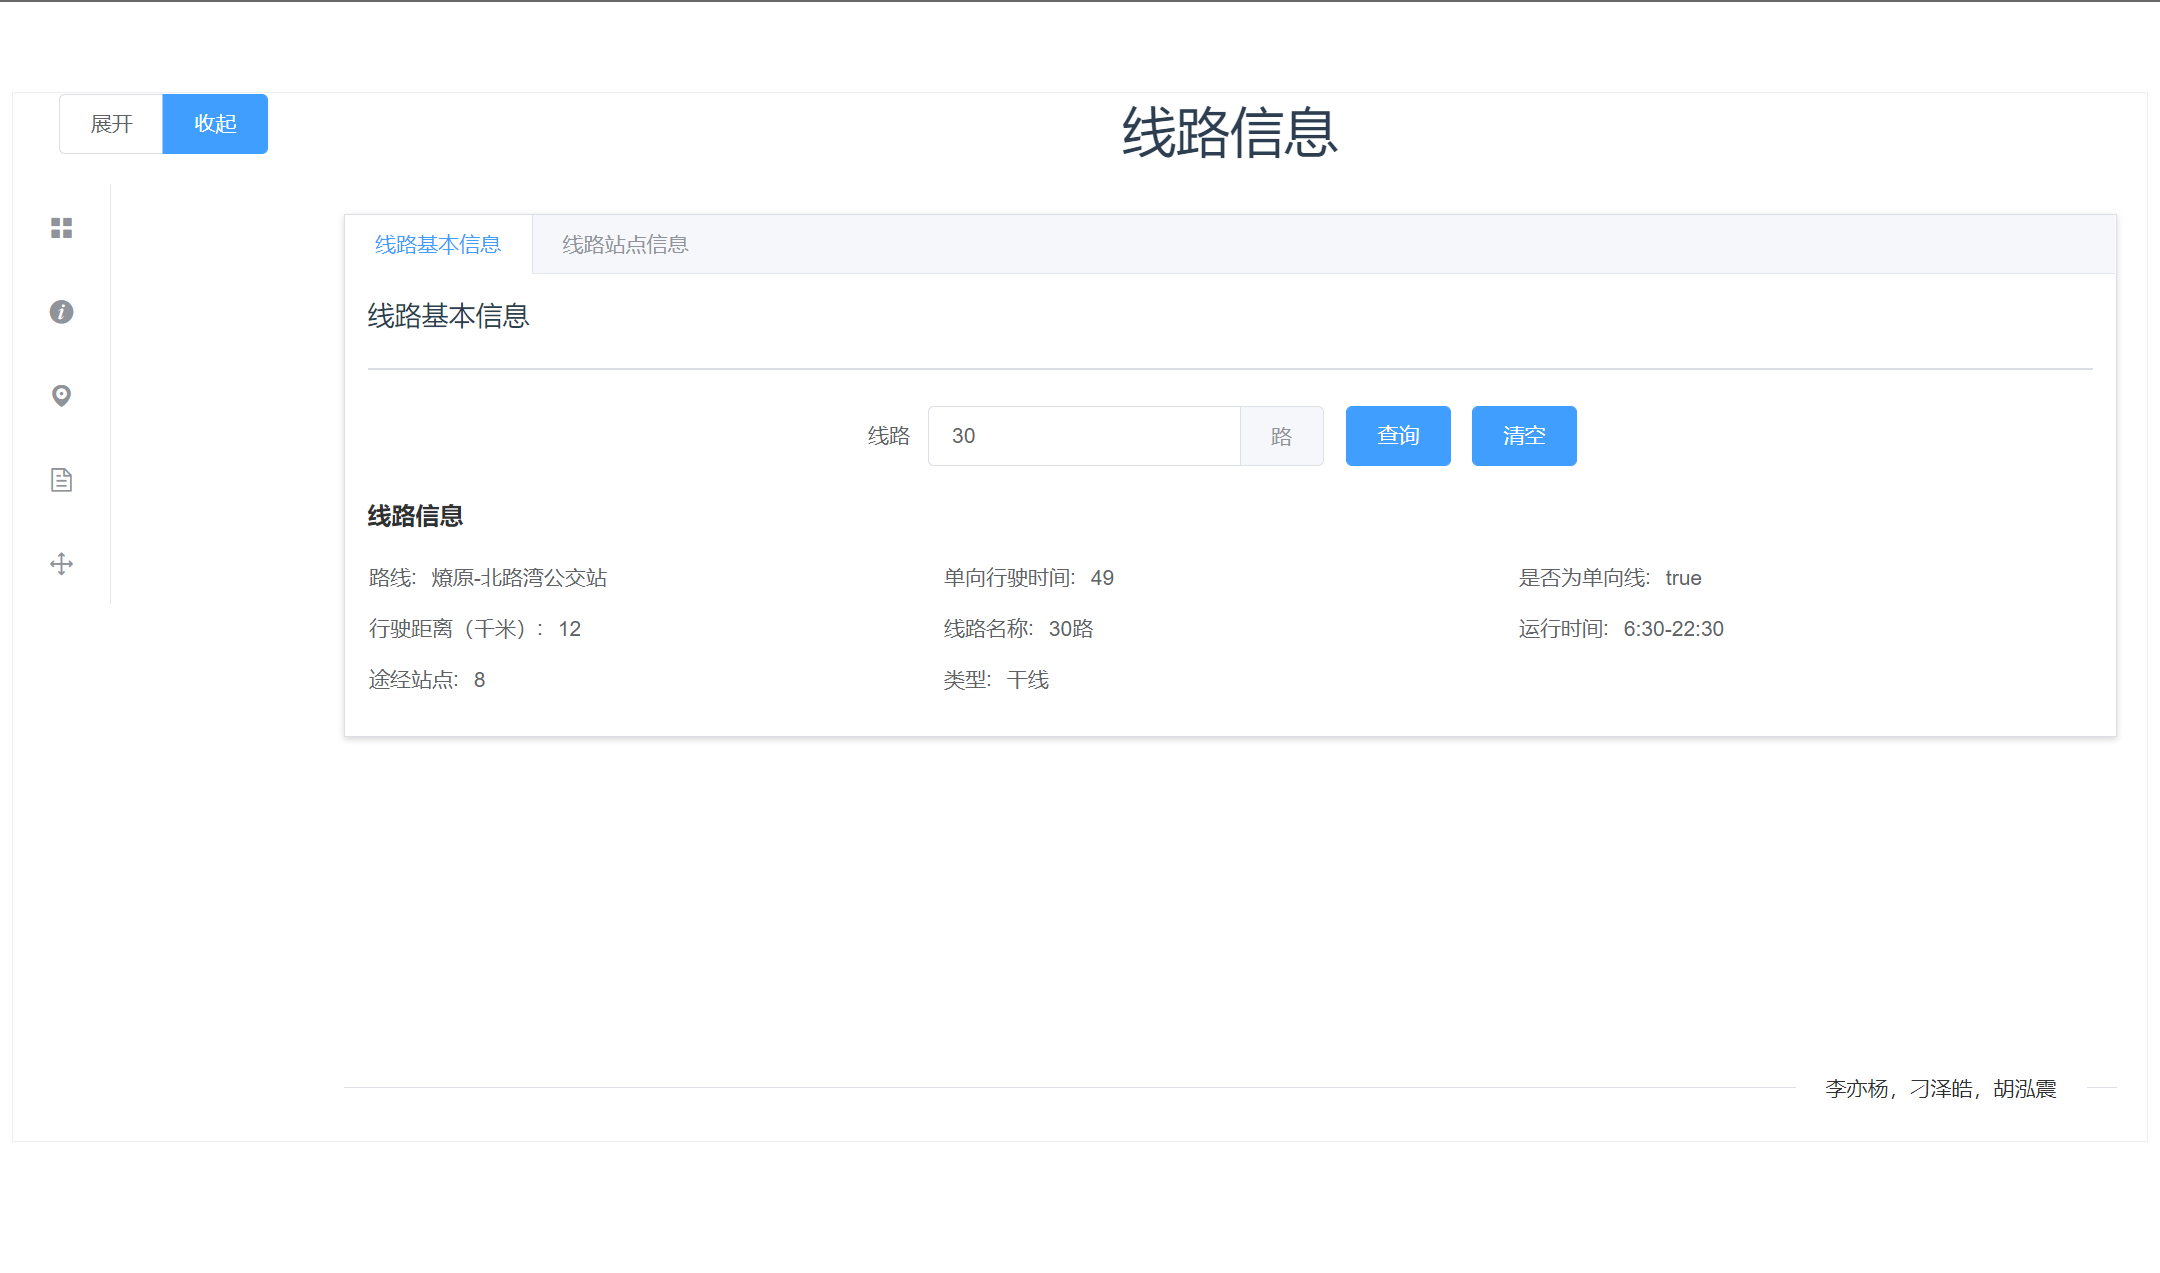
\includegraphics[scale=0.3]{./assets/demand1_1.png} \\ 
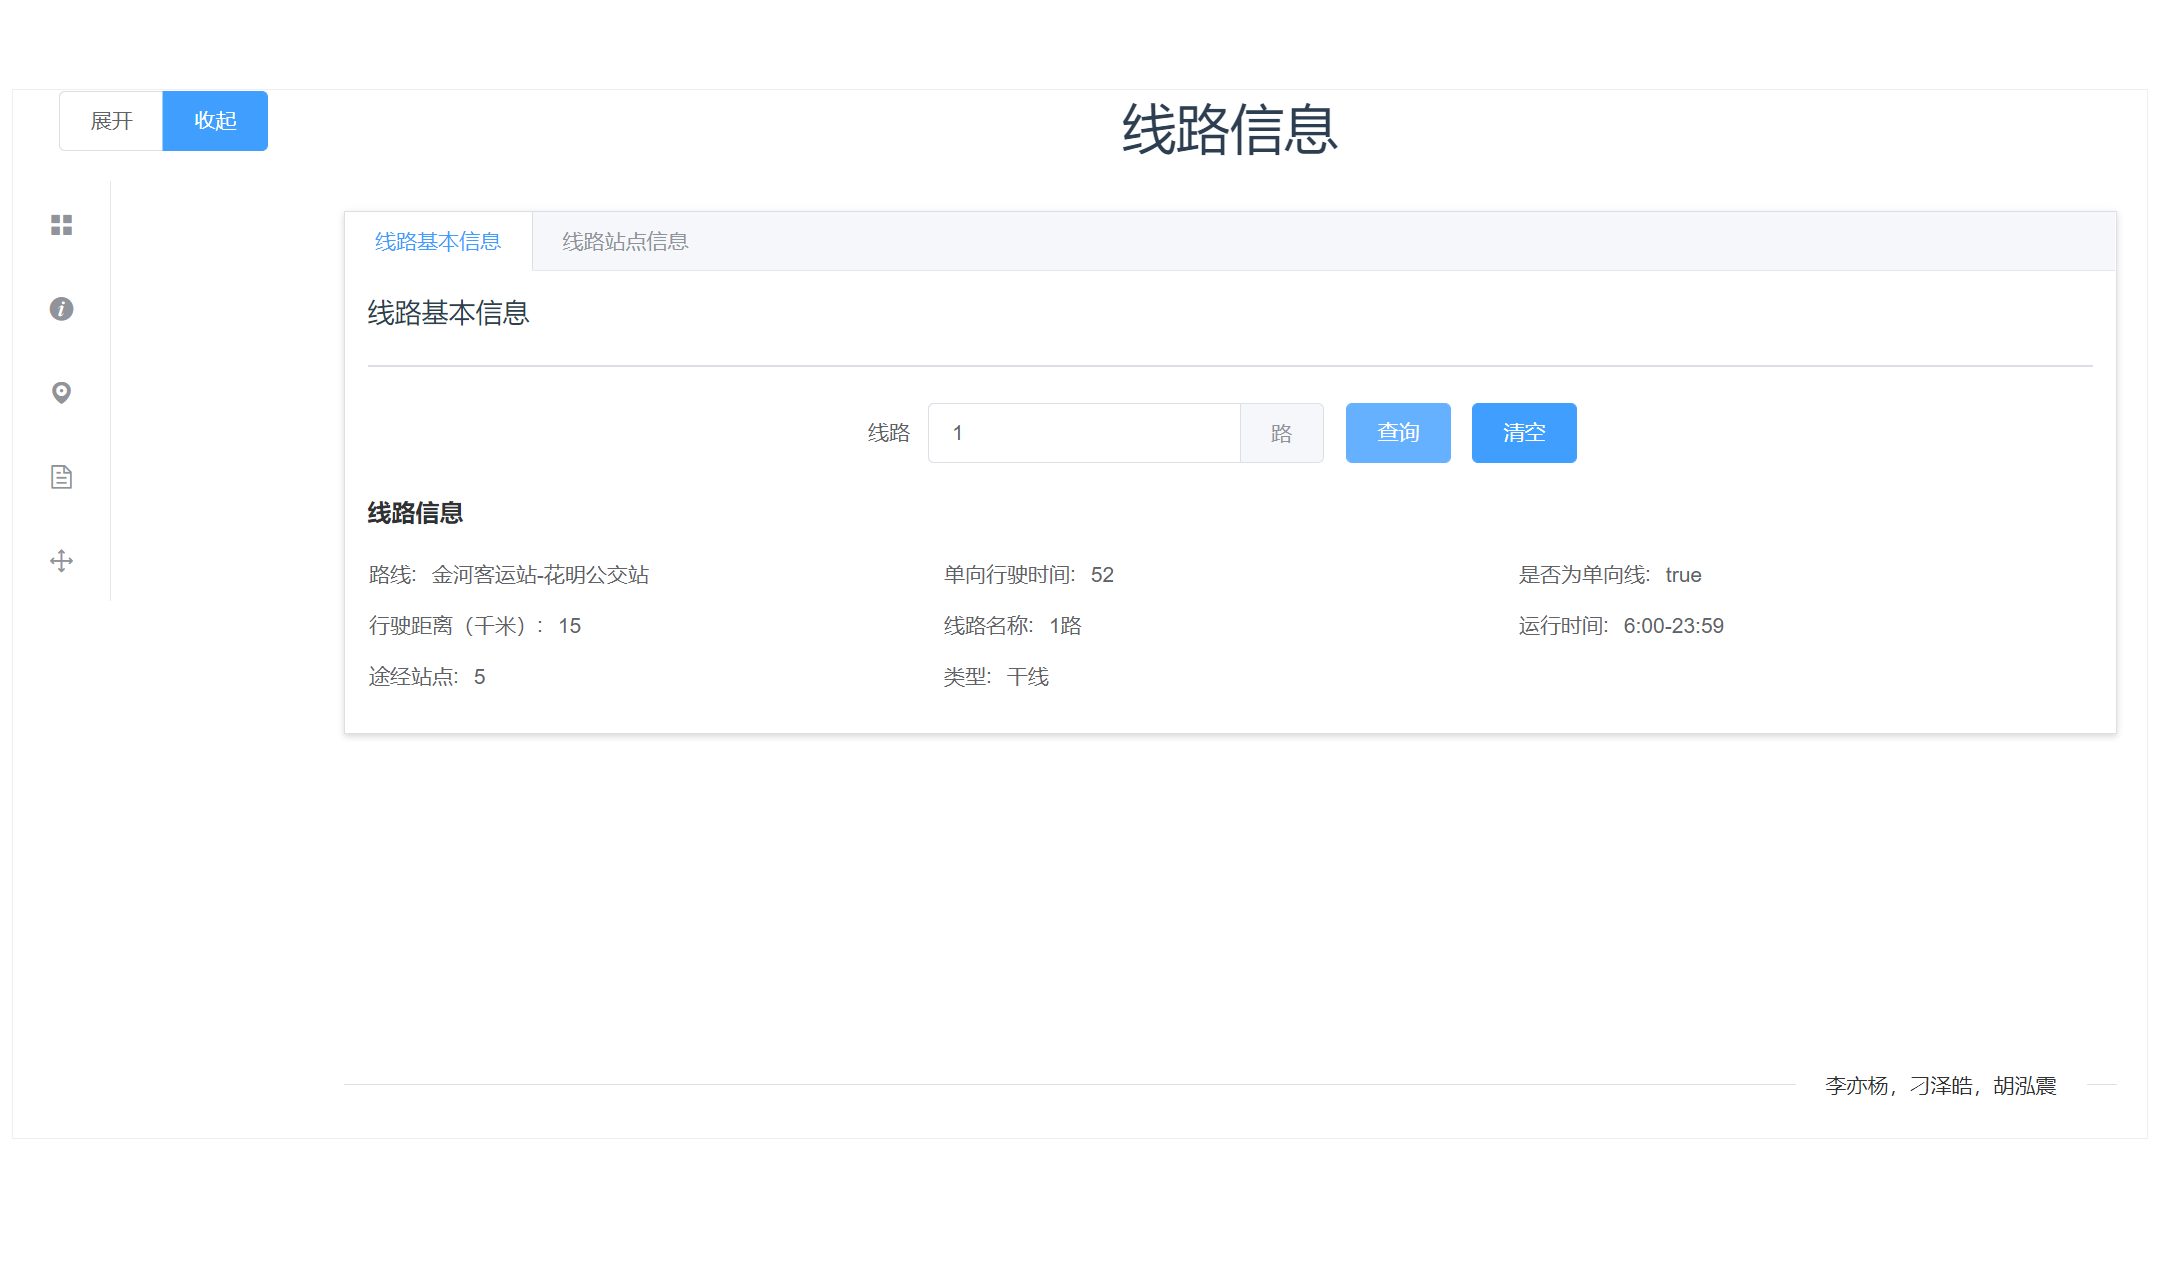
\includegraphics[scale=0.3]{./assets/demand1_2.png} 
\end{center}

\subsection{需求2}
\textbf{要求根据线路名称返回途径站点信息,站点信息对应实体层Station类中的三个属性:id,name,english。} \\
\textbf{Cypher} \\
\begin{lstlisting}[numbers = left, 
showstringspaces=false,
showspaces = false,
breaklines = true, 
language=Java]
@Query("""
	match (l:Line {name: {line_id}, direction: {direction}}) 
	unwind l.route as k
	match (s:Station {id: k})
	return s""")
ArrayList<Station> find_route_station(String line_id, String direction
\end{lstlisting} 
匹配到对应的Line节点后,通过route属性查询对应站点并返回。

\textbf{业务层} \\
\begin{lstlisting}[numbers = left, 
showstringspaces=false,
showspaces = false,
breaklines = true, 
language=Java]
    public JSONArray find_route_station(String line_id,String direction){
        JSONArray arr = new JSONArray();
        ArrayList<Station> station;
        station = stationrepository.find_route_station(line_id, direction);
        if(!station.isEmpty()){
            for(int i = 0; i<station.size();i++)
            {
                JSONObject obj = new JSONObject();
                Station s = station.get(i);
                obj.put("id",s.getId());
                obj.put("name",s.getName());
                obj.put("english",s.getEnglish());
                arr.add(obj);
            }
        }
        return arr;
    }
\end{lstlisting} 
调用StationRepository中的find$\_$route$\_$station函数,返回一个ArrayList<Station>。由于途径多个站点,返回一个JSONArray对象,其中的每个JSONObject对应一个Station列表中的一项。

\textbf{前端界面测试结果} \\
\begin{center}
\centering
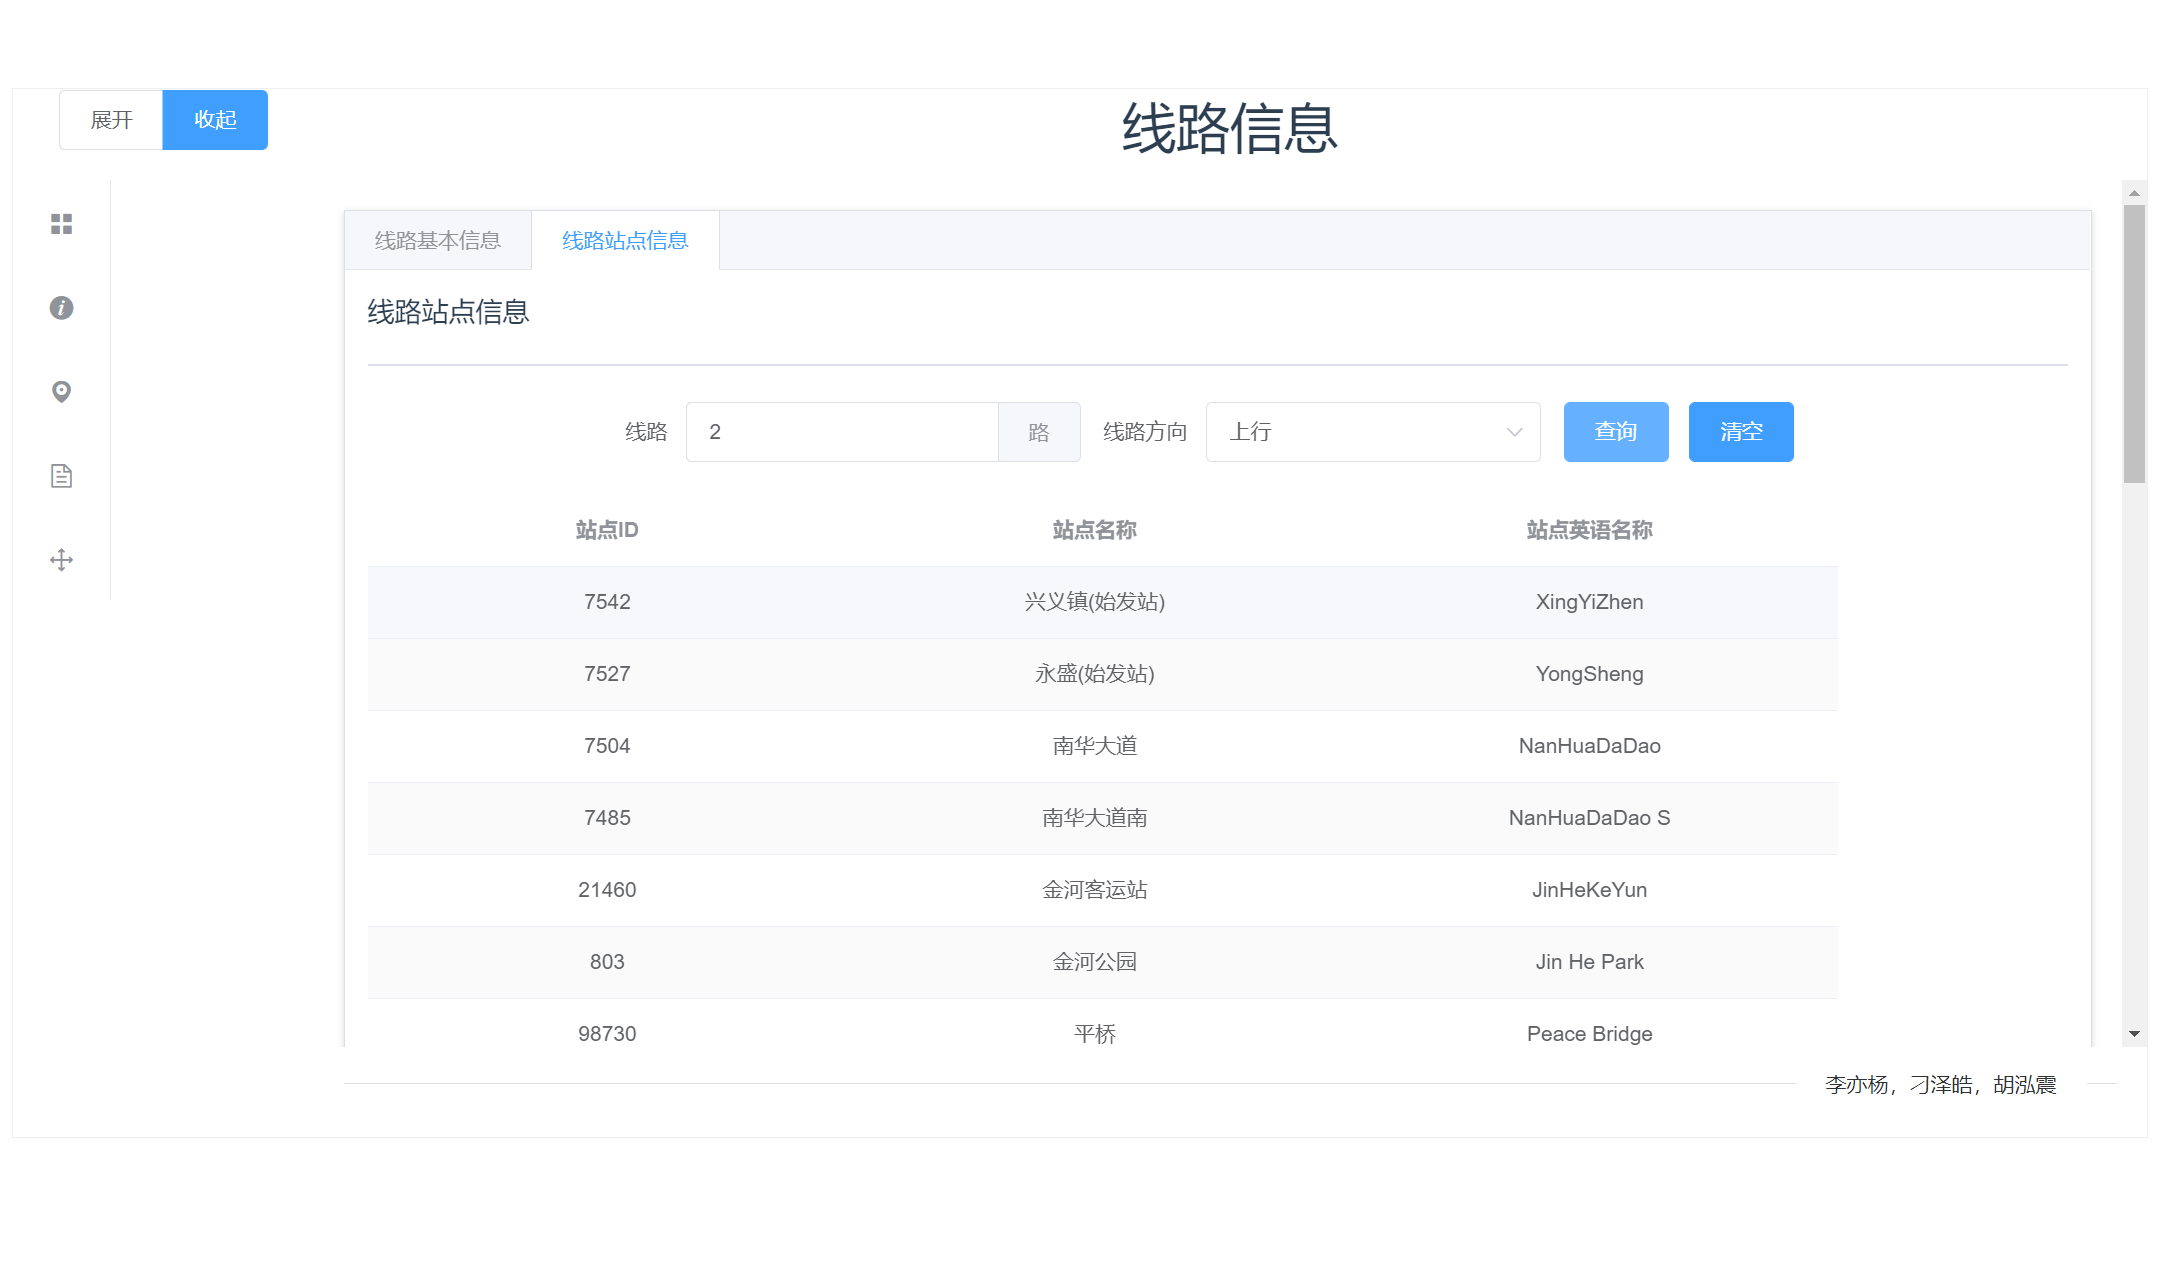
\includegraphics[scale=0.3]{./assets/demand2_1.png} \\ 
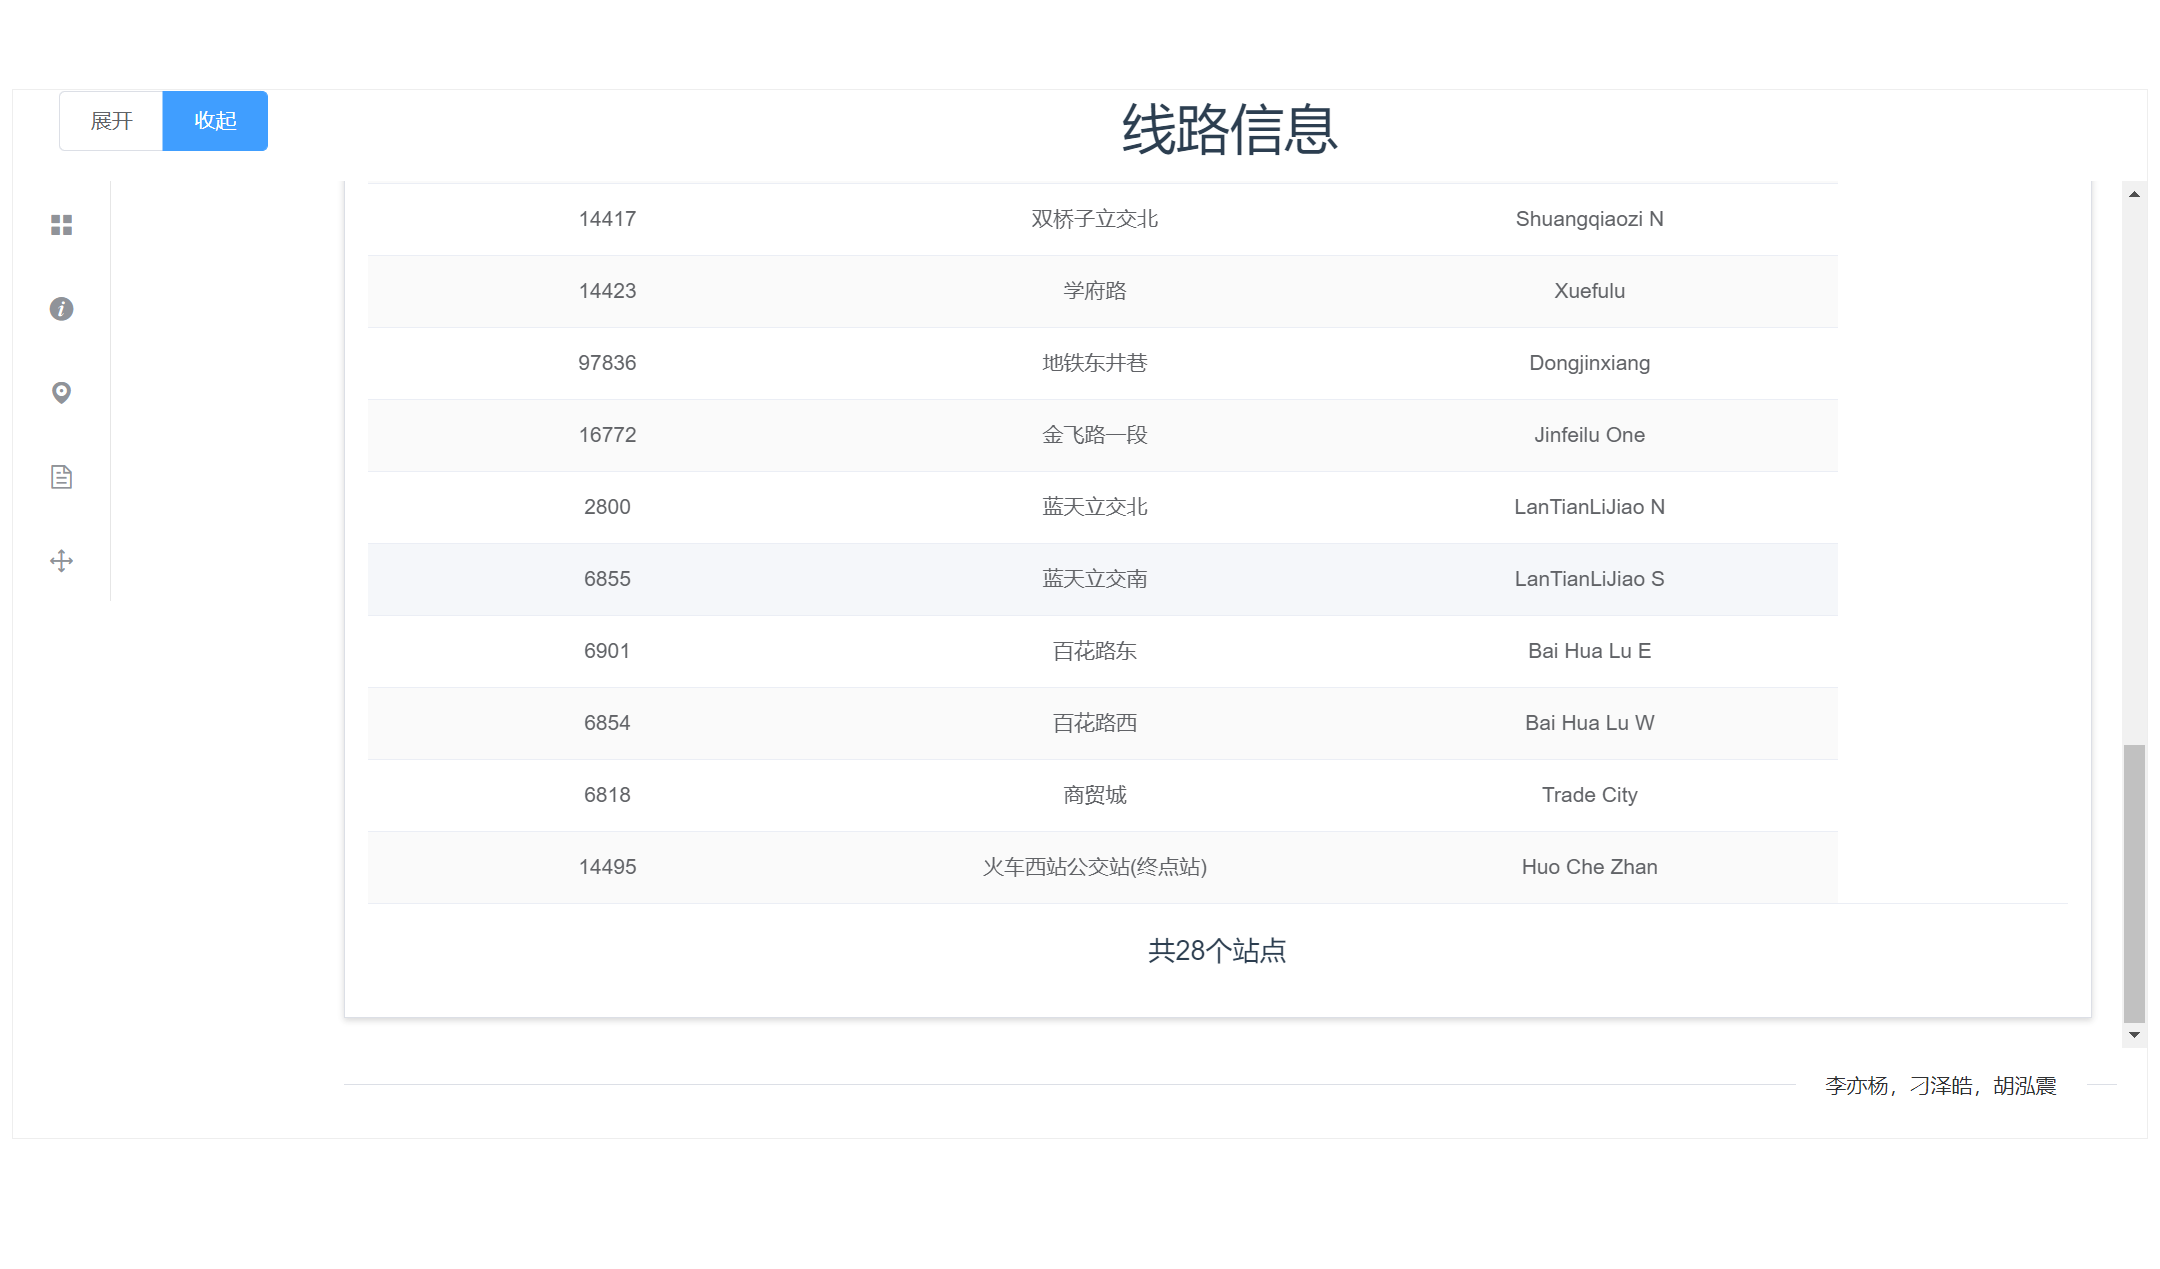
\includegraphics[scale=0.3]{./assets/demand2_2.png} \\ 
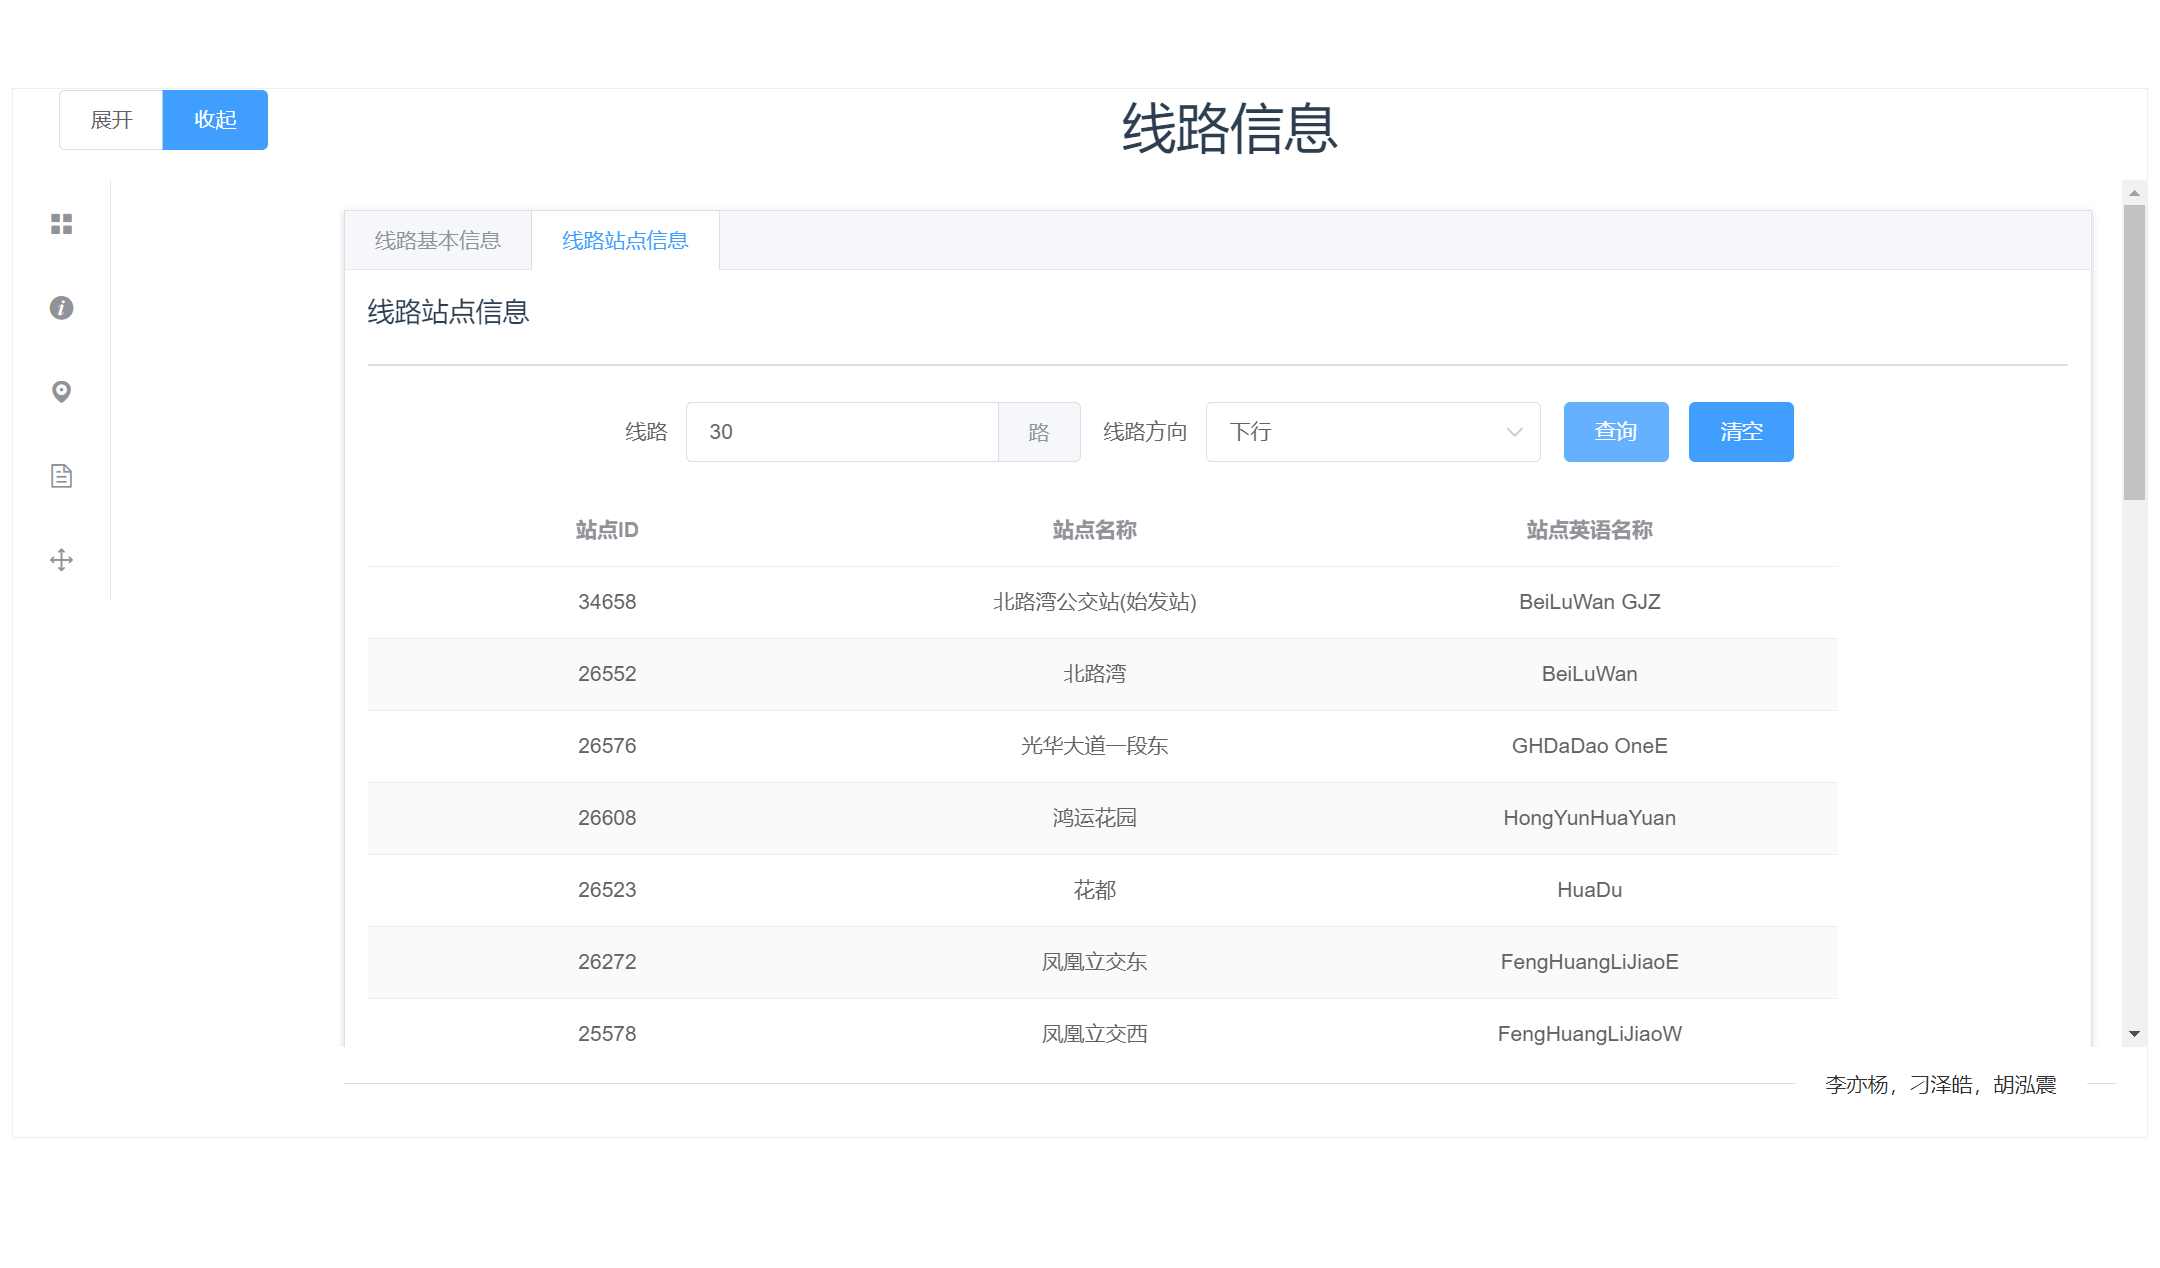
\includegraphics[scale=0.3]{./assets/demand2_3.png} \\ 
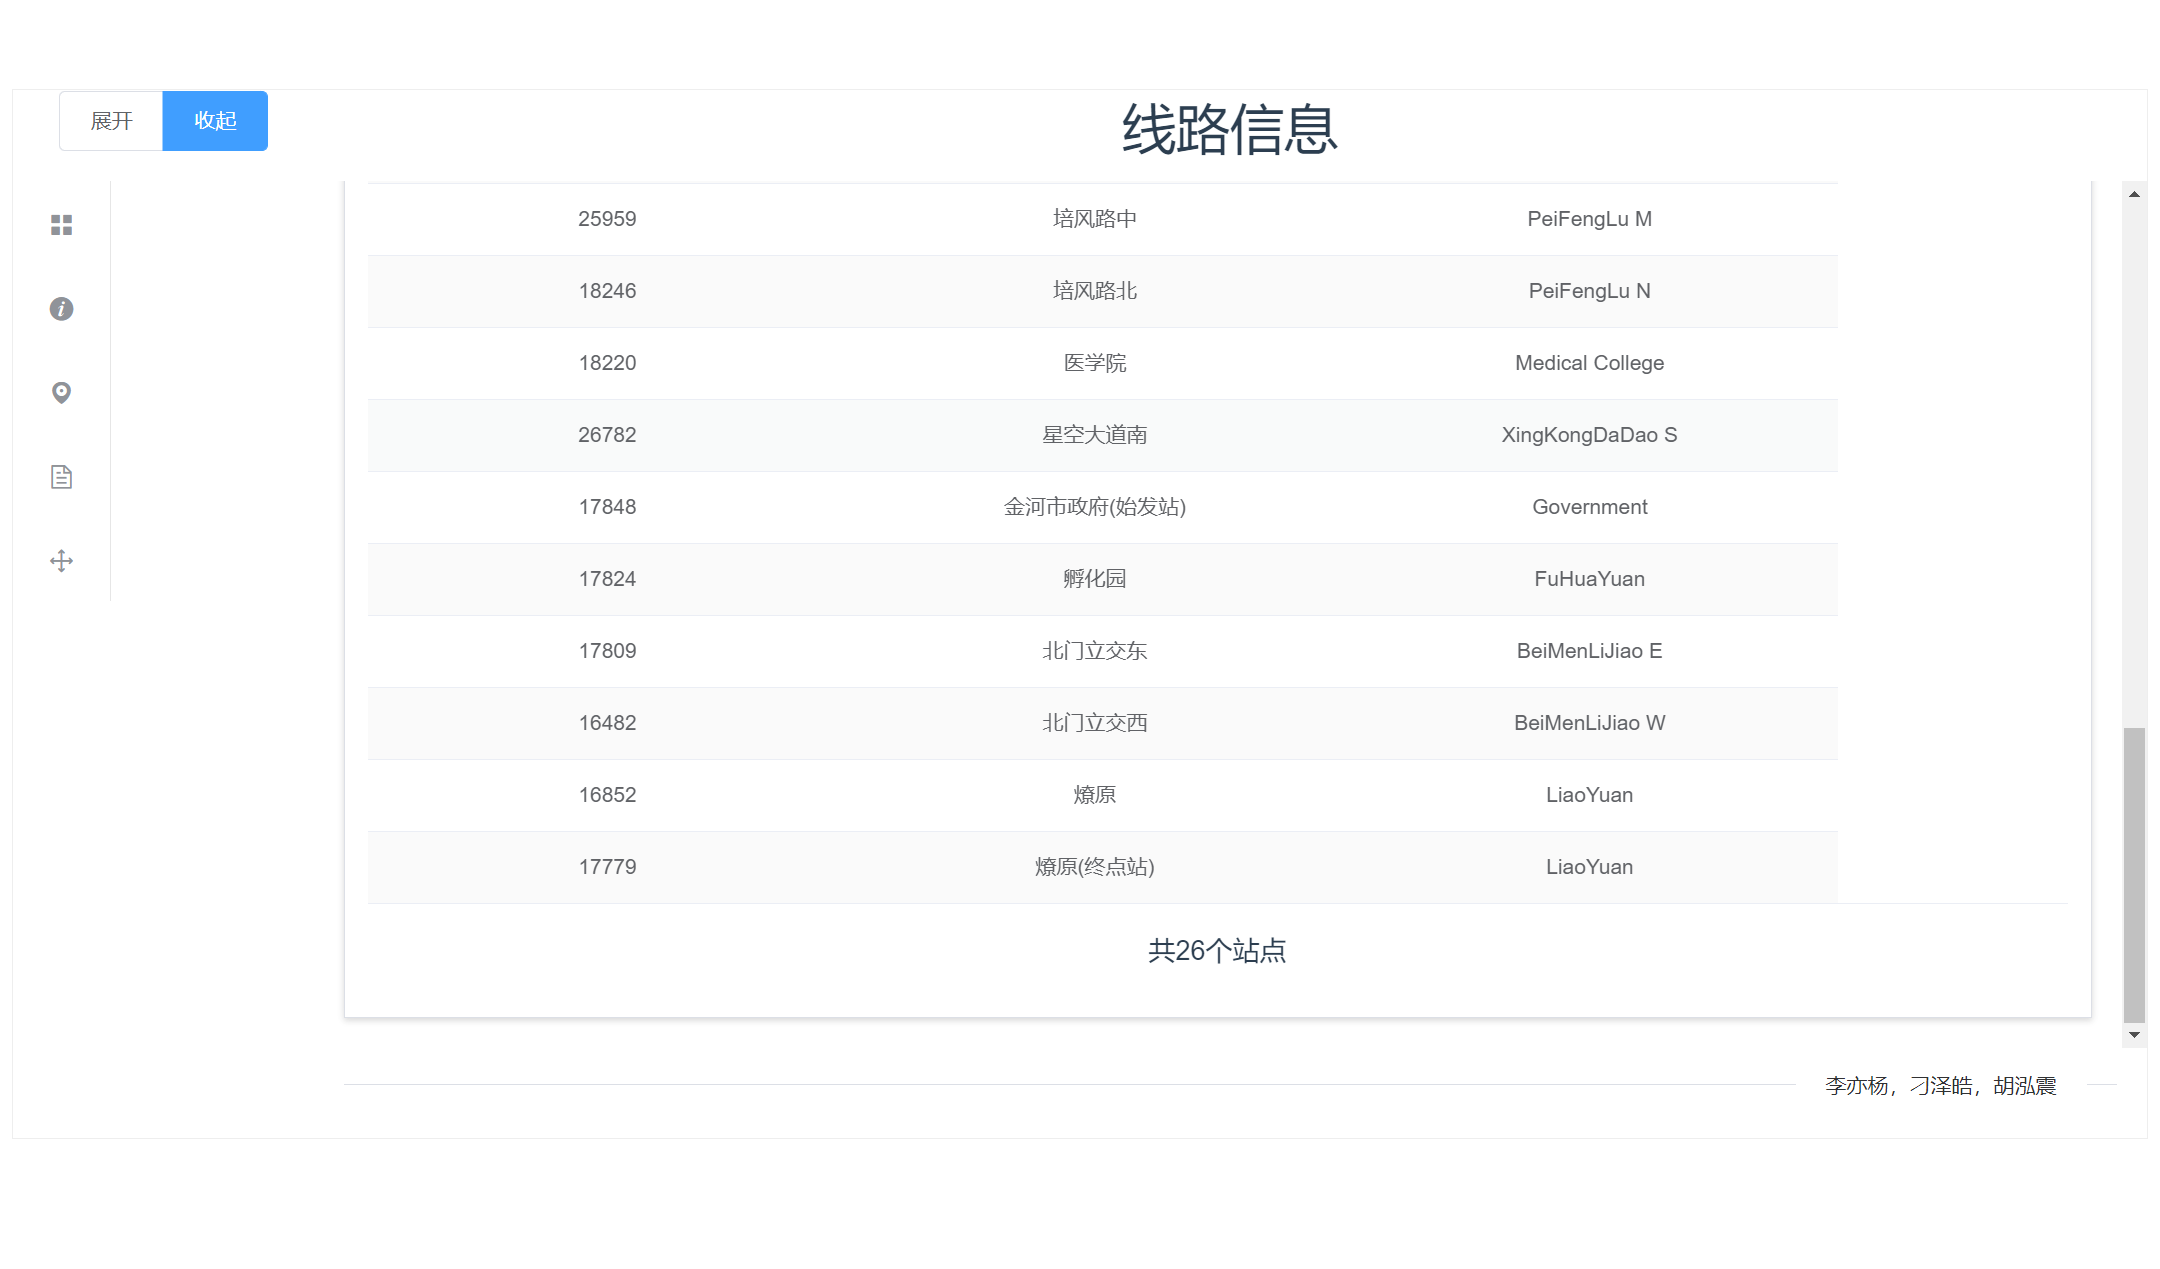
\includegraphics[scale=0.3]{./assets/demand2_4.png} 
\end{center}

\subsection{需求3}
\textbf{根据车站名称返回停靠的线路信息(区分上下行),若车站名字存在重复,则按车站id进行分组。} \\
\textbf{Cypher} \\
\begin{lstlisting}[numbers = left, 
showstringspaces=false,
showspaces = false,
breaklines = true, 
language=Java]
@Query("""
	match (s:Station {name: {station_name}})
	return distinct s.id
	""")
ArrayList<String> find_stationName_routeName_stationId(String station_name);

@Query("""
	match (s:Station {id: {station_id}}) -[r]- ()
	match (l:Line) where l.name in r.lines and s.id in l.route
	return distinct l.name + l.direction
	""")
ArrayList<String> find_stationName_routeName_lineId(String station_id);
\end{lstlisting} 
第一个函数接受站名返回站ID。 \\
第二个函数接受站ID,查询route属性中存在该ID的Line节点。这些节点就是停靠该站的,然后将它们返回。

\textbf{业务层} \\
\begin{lstlisting}[numbers = left, 
showstringspaces=false,
showspaces = false,
breaklines = true, 
language=Java]
    public JSONArray find_stationName_routeName(String stationName){
        JSONArray arr = new JSONArray();
        ArrayList<String> res_stationId = stationrepository.find_stationName_routeName_stationId(stationName);

        ArrayList<ArrayList<String>> res_lineId = new ArrayList<>();

        if(!res_stationId.isEmpty()){

            for(int i = 0; i < res_stationId.size(); i ++){
                String tmpid = res_stationId.get(i);
                ArrayList<String> tmpres_lineId_t =  stationrepository.find_stationName_routeName_lineId(tmpid);

                ArrayList<String> tmpres_lineId = new ArrayList<>();

                if(!tmpres_lineId_t.isEmpty()){
                    for(int k = 0; k < tmpres_lineId_t.size(); k ++){
                        String tmp = tmpres_lineId_t.get(k);
                        if(tmp.contains("up"))
                            tmp = tmp.replace("up", "路上行");
                        else if(tmp.contains("down"))
                            tmp = tmp.replace("down", "路下行");
                        else if(tmp.contains("circle"))
                            tmp = tmp.replace("circle", "路环线");

                        tmpres_lineId.add(tmp);
                    }
                }

                res_lineId.add(tmpres_lineId);
            }
        }

        ArrayList<Demand3> result = new ArrayList<>();

        if(!res_stationId.isEmpty()){
            for(int i = 0; i < res_stationId.size(); i ++){
                Demand3 dem = new Demand3();
                dem.stationId = res_stationId.get(i);
                dem.lineIds = res_lineId.get(i);
                result.add(dem);
            }
        }

        if(!result.isEmpty()){
            for(int i=0;i<result.size();i++)
            {
                JSONObject obj = new JSONObject();
                Demand3 demand3 = new Demand3();
                demand3 = result.get(i);
                obj.put("id",demand3.stationId);
                String str = "";
                ArrayList<String> lineIds;
                lineIds =demand3.lineIds;
                if(!lineIds.isEmpty()){
                    for(int j = 0 ; j < lineIds.size() ; j++)
                    {
                        str += "\"";
                        str += lineIds.get(j);
                        str += "\" ";
                    }
                }
                obj.put("routes",str);
                arr.add(obj);
            }
        }
        return arr;
    }
\end{lstlisting} 
首先调用StationRepository中的find$\_$stationName$\_$routeName$\_$stationId函数(函数命名有些复杂因为后期debug过程中对函数功能进行了修改),返回ArrayList<String> res$\_$stationId,里面是输入的车站名称对应的所有车站id。\\
然后对res$\_$stationId中的每一项分别调用find$\_$stationName$\_$routeName$\_$lineId和find$\_$stationName$\_$routeName$\_$direction函数,前者返回经过该车站的线路id(是一个ArrayList<String>),后者返回线路方向(也是ArrayList<String>)。将stationId、lineId和direction存入Demand3对象列表中,然后将其转换为JSONArray返回。在转换过程中还涉及了对线路id和方向字符串的拼接。

\textbf{前端界面测试结果} \\
\begin{center}
\centering
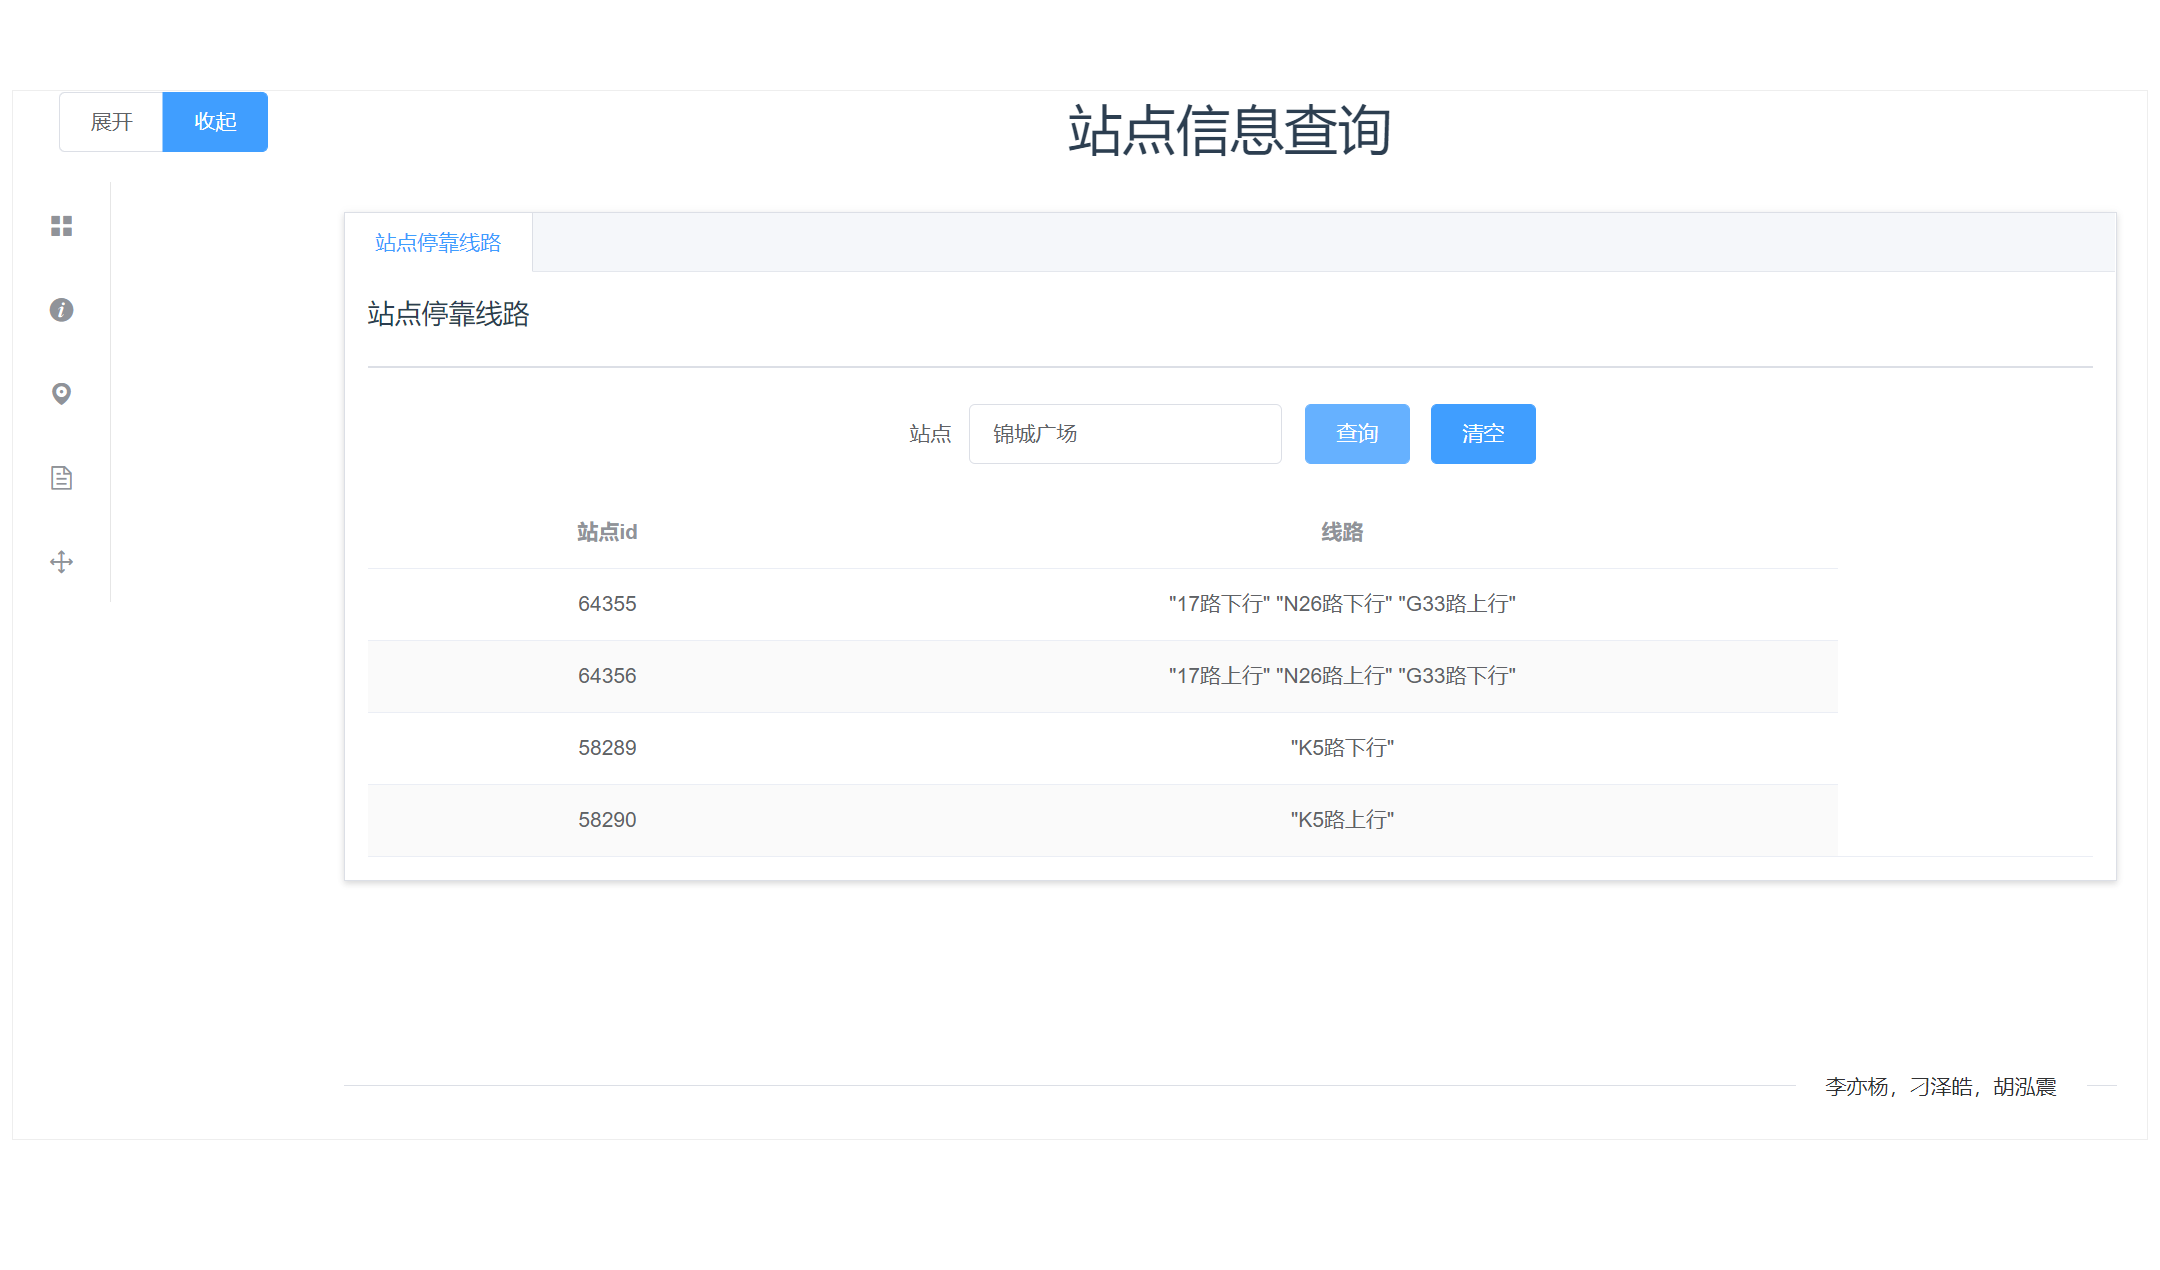
\includegraphics[scale=0.3]{./assets/demand3_1.png} \\ 
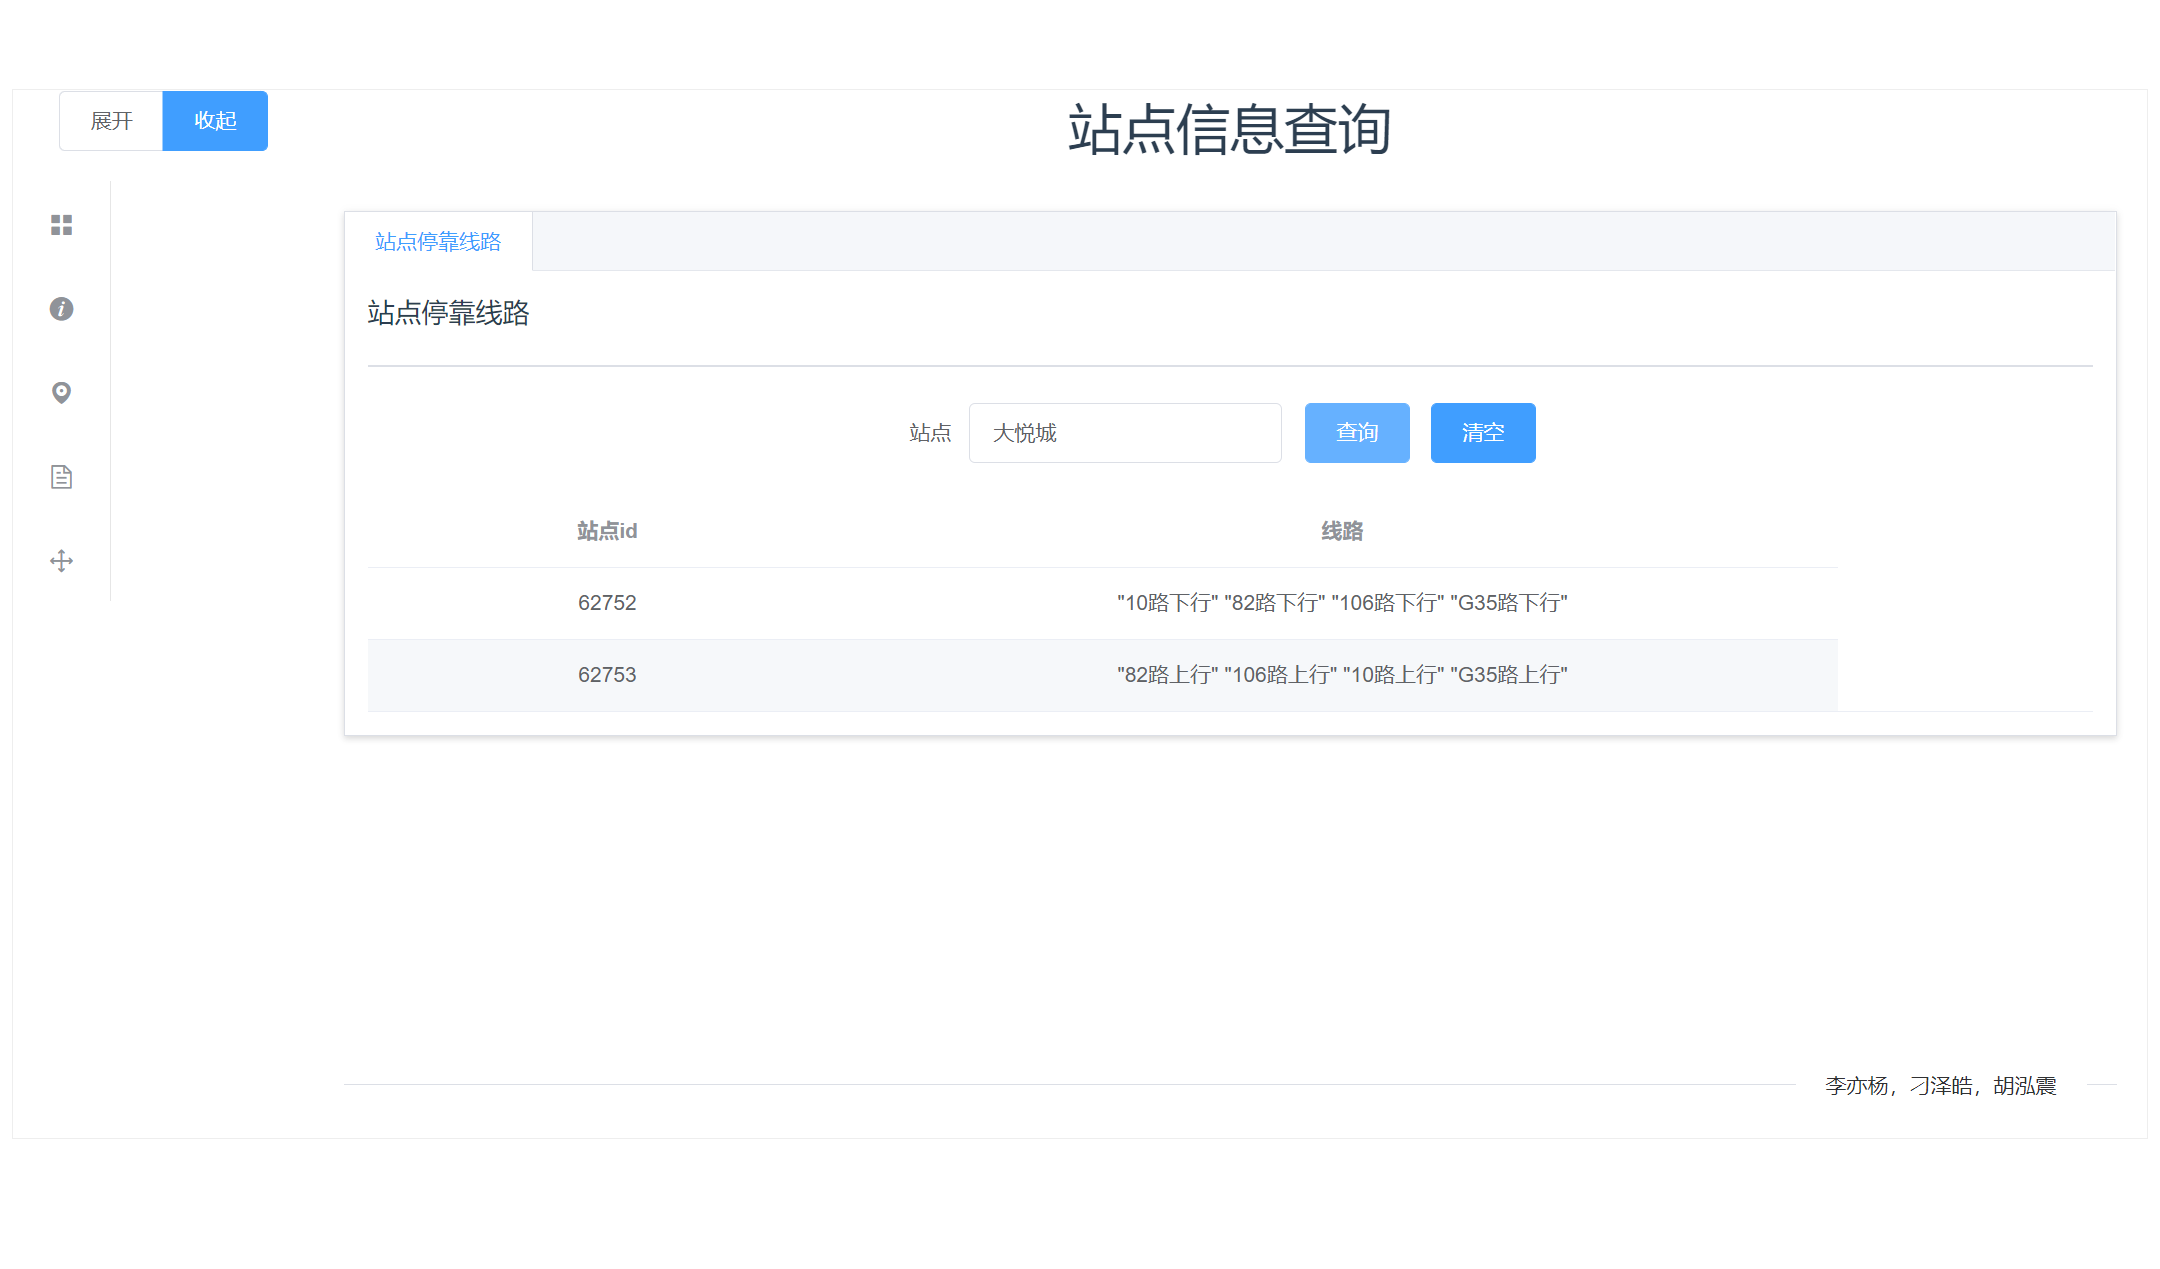
\includegraphics[scale=0.3]{./assets/demand3_2.png} 
\end{center}

\subsection{需求4}
\textbf{根据要乘坐的路线代号和起止站点,返回线路运行方向、途径站点、运行时长。} \\
\textbf{Cypher} \\
\begin{lstlisting}[numbers = left, 
showstringspaces=false,
showspaces = false,
breaklines = true, 
language=Java]
@Query("""
	match (l:Line {name: {line_id}, direction: {direction}})
	unwind l.route as k
	match (s:Station {id: k})
	return s""")
ArrayList<Station> find_route_station(String line_id, String direction);
\end{lstlisting} 
首先通过站名查出站ID,然后通过route属性匹配先经过起点后经过终点的Line。再通过Line查到对应的一个Run节点,从Run节点中取出到达两站的时间。最后返回站名、方向,到达起点和终点的时刻,以及交给service层遍历用的起点和终点在route中的索引。 \\
然后,service通过第二个函数查询起点和终点之间的每个站。

\textbf{业务层} \\
\begin{lstlisting}[numbers = left, 
showstringspaces=false,
showspaces = false,
breaklines = true, 
language=Java]
public JSONObject find_lineId_stationName_path(String lineId,String stationName1,String stationName2){
        JSONObject obj = new JSONObject();
        Demand4 result = new Demand4();

        String res_lineName = linerepository.find_lineId_stationName_path_lineName(lineId, stationName1, stationName2);
        String res_direction = linerepository.find_lineId_stationName_path_direction(lineId, stationName1, stationName2);
        String res_depttime = linerepository.find_lineId_stationName_path_departtime(lineId, stationName1, stationName2);
        String res_desttime = linerepository.find_lineId_stationName_path_desttime(lineId, stationName1, stationName2);
        int res_deptind = linerepository.find_lineId_stationName_path_departind(lineId, stationName1, stationName2);
        int res_destind = linerepository.find_lineId_stationName_path_destind(lineId, stationName1, stationName2);

        String res_direct = new String();
        if(Objects.equals(res_direction, "up"))
            res_direct = "上行";
        else if (Objects.equals(res_direction, "down"))
            res_direct = "下行";
        else if (Objects.equals(res_direction, "circle"))
            res_direct = "环线";

        result.lineName = res_lineName;
        result.direction = res_direction;
        result.departure_time = res_depttime;
        result.destination_time = res_desttime;
        result.departure_index = res_deptind;
        result.destination_index = res_destind;

        if(result != null){
            obj.put("lineName",result.lineName + "路" + res_direct);
            SimpleDateFormat ft = new SimpleDateFormat ("HH:mm");
            Date t1;
            long l1;
            Date t2;
            long l2;
            int runtime;
            if((!(result.departure_time==null))&&(!(result.destination_time==null)))
            {
                try{
                    t1 = ft.parse(result.destination_time);
                    l1 = t1.getTime();
                    t2 = ft.parse(result.departure_time);
                    l2 = t2.getTime();
                    runtime = (int)((l1 - l2)/60000);
                    obj.put("runTime",runtime);
                }catch (ParseException e){
                    System.out.println("Unparseable using " + ft);
                }
            }
            JSONArray arr =new JSONArray();
            int departure_index = result.departure_index;
            int destination_index = result.destination_index;
            for(int i = departure_index;i<=destination_index;i++)
            {
                Station sta = stationrepository.find_route_station_by_index(result.lineName,result.direction,i);
                JSONObject s = new JSONObject();
                s.put("id",sta.getId());
                s.put("name",sta.getName());
                s.put("english",sta.getEnglish());
                arr.add(s);
            }
            obj.put("stations",arr);
        }

        return obj;
    }
\end{lstlisting} 
创建Demand4类(里面包含String lineName; String direction; String departure$\_$time; String destination$\_$time; int departure$\_$index; int destination$\_$index)的列表result。\\
然后分别调用LineRepository层的函数:
\begin{itemize}
\item find$\_$lineId$\_$stationName$\_$path$\_$lineName
\item find$\_$lineId$\_$stationName$\_$path$\_$direction
\item find$\_$lineId$\_$stationName$\_$path$\_$departtime
\item find$\_$lineId$\_$stationName$\_$path$\_$desttime
\item find$\_$lineId$\_$stationName$\_$path$\_$departind
\item find$\_$lineId$\_$stationName$\_$path$\_$destind 
\end{itemize}
传入的参数都是线路id和起始终止站点名,分别返回站点间线路的名称、方向、到达起始点的时间、到达终止点的时间、起始点的索引值、终止点的索引值。随后根据两个时间点算出线路运行时间,并根据首尾索引遍历他们中间的所有索引值对应的站点信息,并保存在一个JSONArray对象中,最后与运行时间和线路名称整合成一个JSONObject对象返回。

\textbf{前端界面测试结果} \\
\begin{center}
\centering
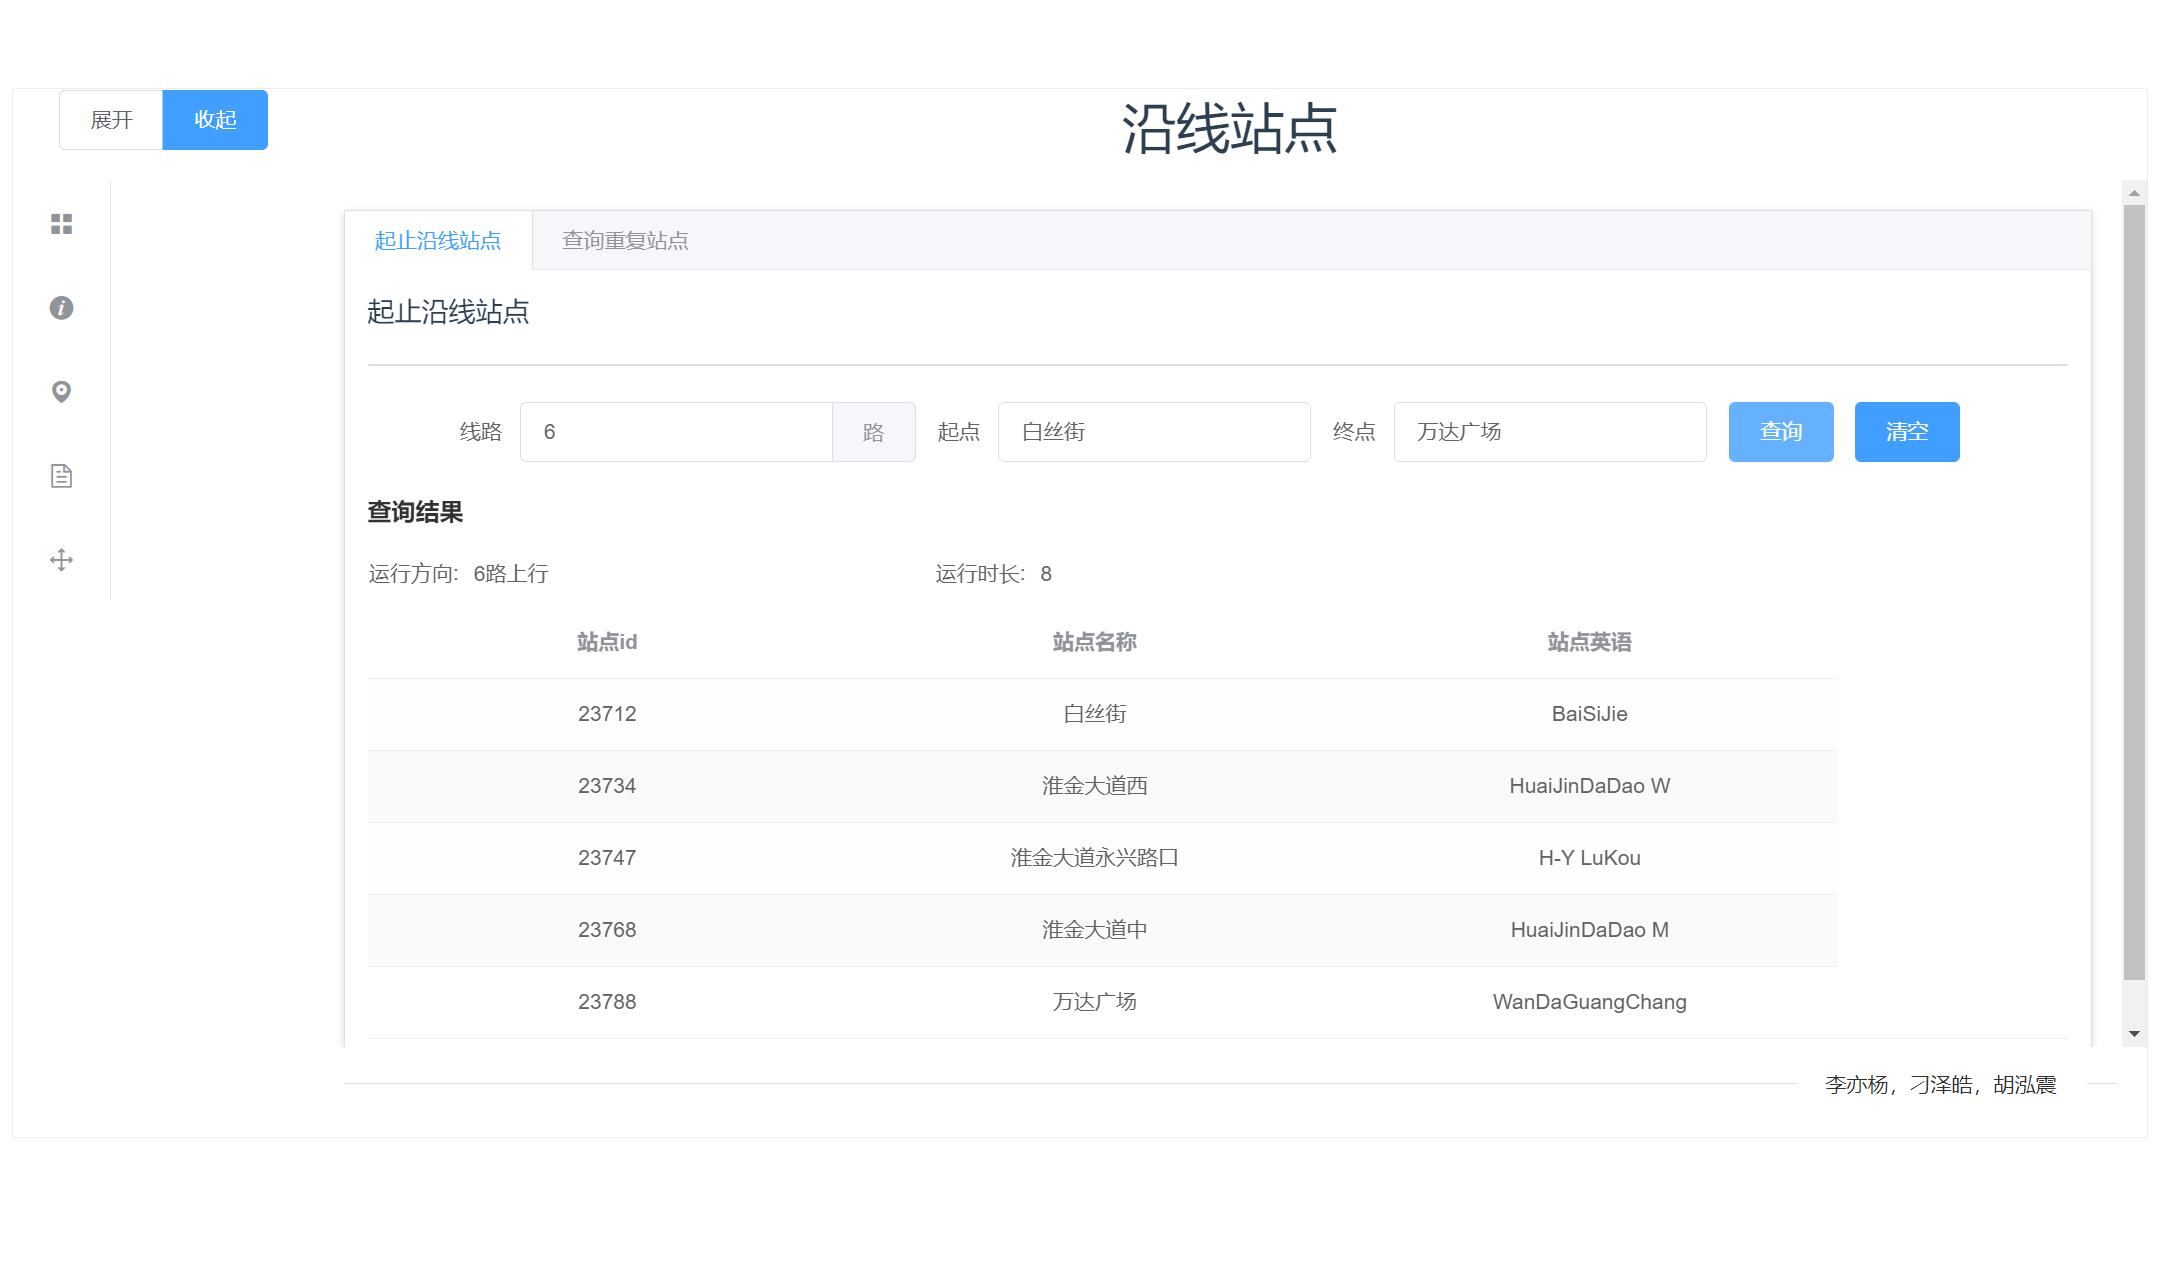
\includegraphics[scale=0.3]{./assets/demand4_1.jpg} \\ 
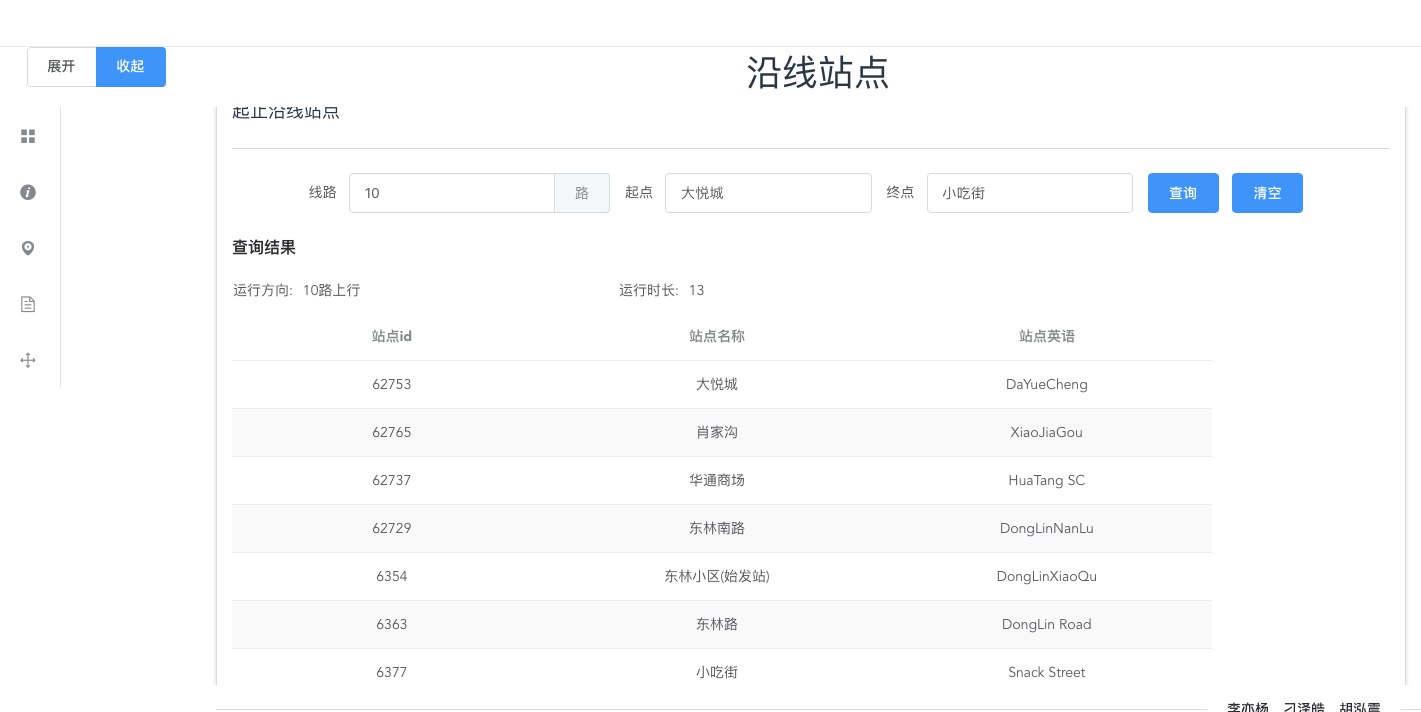
\includegraphics[scale=0.3]{./assets/demand4_2.png} 
\end{center}

\subsection{需求5}
\subsubsection{a}
\textbf{查询某两个站台之间的最短路径,基于ID查询} \\
\textbf{Cypher} \\
\begin{lstlisting}[numbers = left, 
showstringspaces=false,
showspaces = false,
breaklines = true, 
language=Java]
@Query("""
        match (ss:Station{id:{station_id1}}), (se:Station{id:{station_id2}})
        unwind nodes(shortestpath((ss)-[*0..15]-> (se))) as res
        return res.id
    	""")
ArrayList<String> shortestpath_by_id_id(String station_id1, String station_id2);

@Query("""
        match (ss:Station{id:{station_id1}}), (se:Station{id:{station_id2}})
        unwind nodes(shortestpath((ss)-[*0..15]-> (se))) as res
        return res.name
        """)
ArrayList<String> shortestpath_by_id_name(String station_id1, String station_id2);

@Query("""
	match (ss:Station{id:{station_id1}}), (se:Station{id:{station_id2}})
        unwind nodes(shortestpath((ss)-[*0..15]-> (se))) as res
        return res.english
    	""")
ArrayList<String> shortestpath_by_id_eng(String station_id1, String station_id2);
\end{lstlisting} 
Neo4j内置了查询最短路径的函数shortestpath,因而只需通过站点id查询作为出发和目的站点的站点,随后利用shortestpath查询最短路径,并输出结点即可。 \\
由于有的Station关系结点不包含进入方向的关系,有的不包含出方向的关系,因而若直接返回Station实体类会发生映射问题,解决方式是拆分查询语句,并使之返回多个字符串。

\textbf{业务层} \\
\begin{lstlisting}[numbers = left, 
showstringspaces=false,
showspaces = false,
breaklines = true, 
language=Java]
    public JSONArray find_shortestRoute_id(String station1, String station2){
        JSONArray arr = new JSONArray();
        ArrayList<String> station_id;
        station_id = linerepository.shortestpath_by_id_id(station1, station2);
        ArrayList<String> station_name;
        station_name = linerepository.shortestpath_by_id_name(station1, station2);
        ArrayList<String> station_eng;
        station_eng = linerepository.shortestpath_by_id_eng(station1, station2);
        if(!station_id.isEmpty()){
            for(int i = 0; i<station_id.size();i++)
            {
                JSONObject obj = new JSONObject();
                String tmpid = station_id.get(i);
                String tmpname = station_name.get(i);
                String tmpeng = station_eng.get(i);
                obj.put("id",tmpid);
                obj.put("name",tmpname);
                obj.put("english",tmpeng);
                arr.add(obj);
            }
        }
        return arr;
    }
\end{lstlisting} 
逻辑较为简单,与需求6蕾丝,只需要调用三个函数:shortestpath$\_$by$\_$id$\_$id, shortestpath$\_$by$\_$id$\_$name, shortestpath$\_$by$\_$id$\_$eng,再将返回值输出到JSON数组中,最终返回JSON对象即可。

\textbf{前端界面测试结果} \\
\begin{center}
\centering
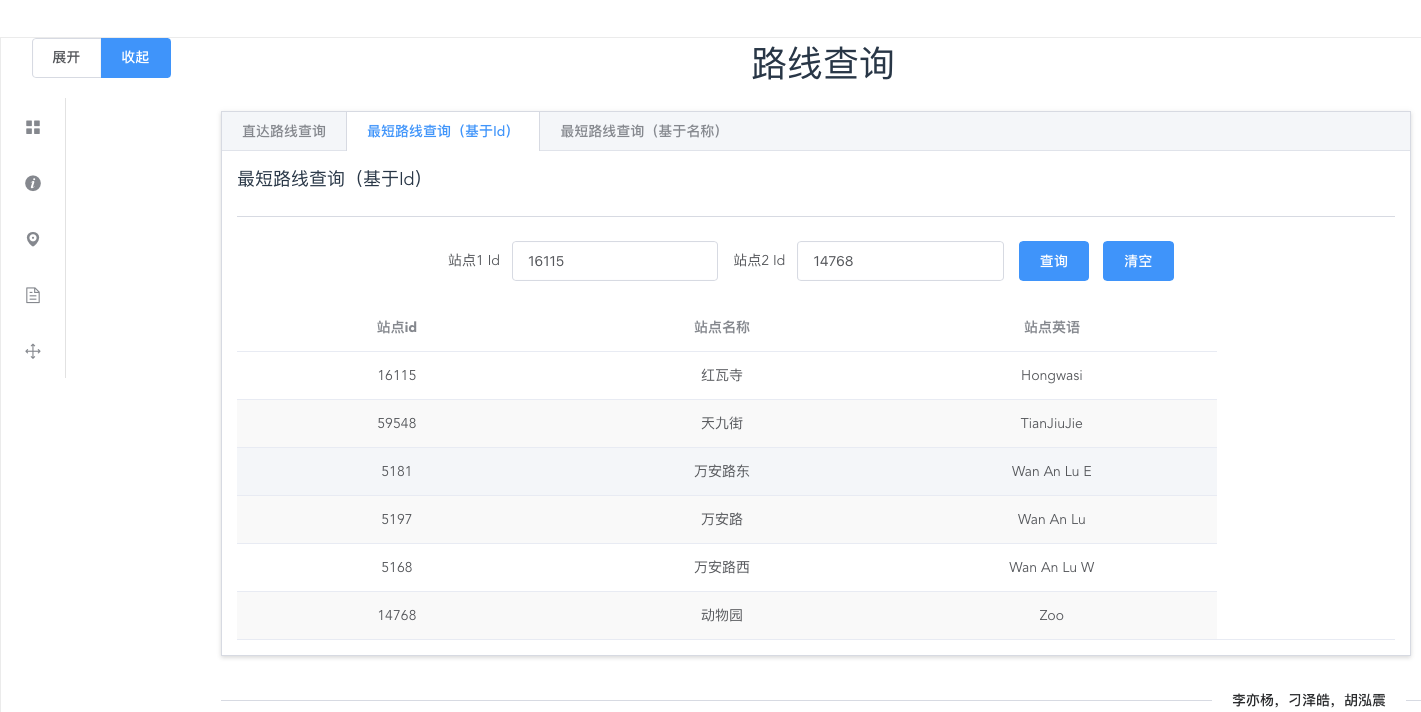
\includegraphics[scale=0.3]{./assets/demand5_1.png} 
\end{center}

\subsubsection{b}
\textbf{查询某两个站台之间的最短路径,基于ID查询} \\
\textbf{Cypher} 名字
\begin{lstlisting}[numbers = left, 
showstringspaces=false,
showspaces = false,
breaklines = true, 
language=Java]
@Query("""
        match (s:Station{name:{station_name}})
        return s.id
    	""")
ArrayList<String> get_all_station_ids_by_name(String station_name);
\end{lstlisting} 
考虑到查询最短路径本质上还是根据站点Id进行查询,因而Cypher层提供一个利用站点名查询所有同名站点Id的函数,其余操作交给业务层完成。

\textbf{业务层} \\
\begin{lstlisting}[numbers = left, 
showstringspaces=false,
showspaces = false,
breaklines = true, 
language=Java]
    public JSONArray find_shortestRoute_name(String station1, String station2){
        JSONArray arr = new JSONArray();
        ArrayList<String> station1_id = linerepository.get_all_station_ids_by_name(station1);
        ArrayList<String> station2_id = linerepository.get_all_station_ids_by_name(station2);
        ArrayList<Station> routes = new ArrayList<>();

        int count = Integer.MAX_VALUE;

        if(!station1_id.isEmpty()){
            if(!station2_id.isEmpty()){
                for(int i = 0; i < station1_id.size(); i ++){
                    for(int j = 0; j < station2_id.size(); j ++){
                        ArrayList<String> tmpids = linerepository.shortestpath_by_id_id(station1_id.get(i), station2_id.get(j));
                        ArrayList<String> tmpnames = linerepository.shortestpath_by_id_name(station1_id.get(i), station2_id.get(j));
                        ArrayList<String> tmpengs = linerepository.shortestpath_by_id_eng(station1_id.get(i), station2_id.get(j));

                        ArrayList<Station> tmproutes = new ArrayList<>();

                        for(int k = 0; k < tmpids.size(); k ++){
                            Station tmps = new Station();
                            tmps.setId(tmpids.get(k));
                            tmps.setName(tmpnames.get(k));
                            tmps.setEnglish(tmpengs.get(k));

                            tmproutes.add(tmps);
                        }

                        if(tmproutes.size() != 0 && tmproutes.size() < count){
                            count = tmproutes.size();
                            routes = tmproutes;
                        }
                    }
                }


            }
        }

        if(!routes.isEmpty()){
            for(int i = 0; i<routes.size();i++)
            {
                JSONObject obj = new JSONObject();
                Station s = routes.get(i);
                obj.put("id",s.getId());
                obj.put("name",s.getName());
                obj.put("english",s.getEnglish());
                arr.add(obj);
            }
        }
        return arr;
    }
\end{lstlisting} 
我们对需求的理解是,对同名站点A, B,以及另一站点C而言,倘若A C间存在路径ac,B C间存在路径bc,则选择ac与bc中较短的输出,换言之总是保证结果只有一条路径。 \\
总体上来说,业务层维护三个ArrayList,routes用来存储最终答案,而另两个则用来存储起点终点站的全部同名站点Id。随后利用两次for循环,为每一组(起点站,终点站)进行最短路线查询。同时设置一个int型变量,初始值位Integer.MAX$\_$VALUE,用于辅助检测最短路径,倘若在一次循环中所查出的路径所含站点数比该变量小,就将该变量重新赋值,并将此次循环查处的路径存储到routes。由此便可以得到最短路径。 \\
最后将routes内站点封装进入JSON对象,并返回。

\textbf{前端界面测试结果} \\
\begin{center}
\centering
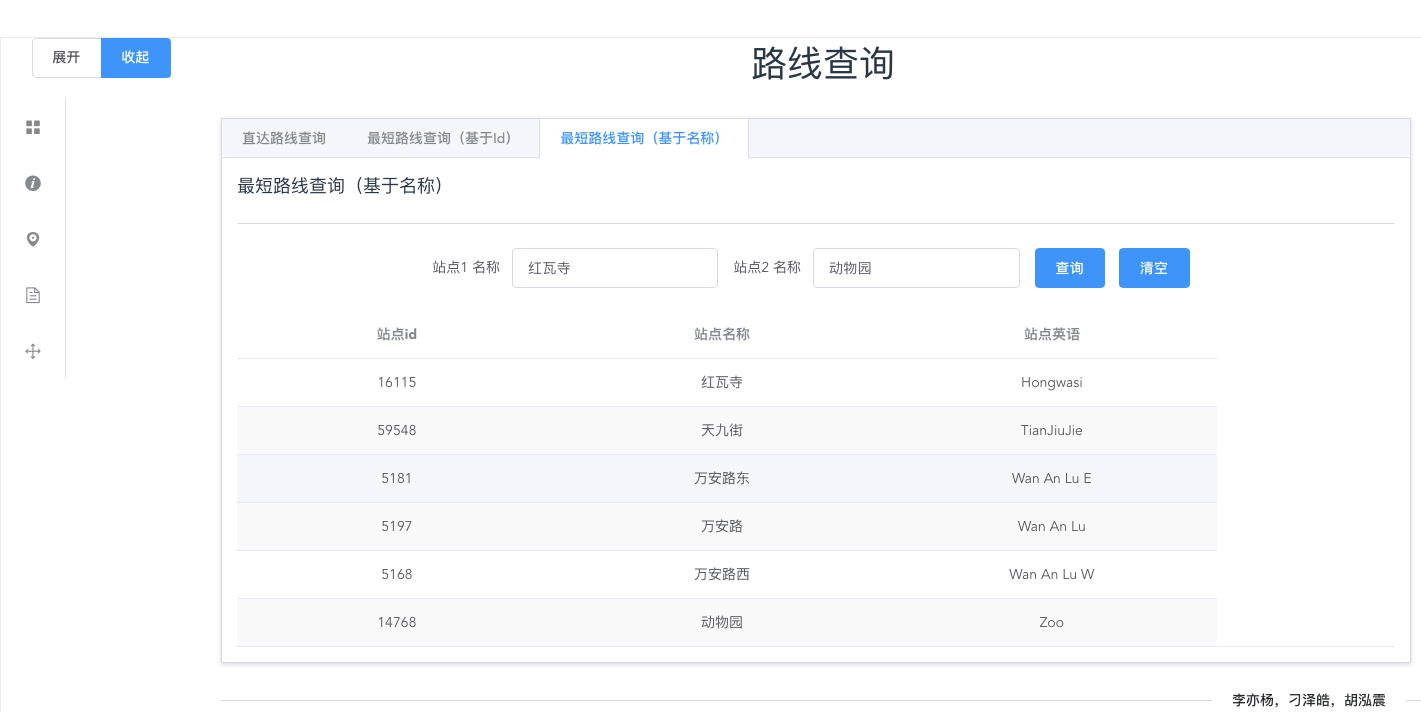
\includegraphics[scale=0.3]{./assets/demand5_2.png} 
\end{center}

\subsection{需求6}
\textbf{根据起止站点名称查询是否存在直达线路,如果有返回线路名称及方向,如果没有返回提示信息。} \\
\textbf{Cypher} \\
\begin{lstlisting}[numbers = left, 
showstringspaces=false,
showspaces = false,
breaklines = true, 
language=Java]
@Query("""
	match (s1:Station{name:{station1}}), (s2:Station{name:{station2}})
	with s1.id as departure, s2.id as destination
	match
		(l:Line) where apoc.coll.indexOf(l.route, departure) > 0 and apoc.coll.indexOf(l.route, departure) < apoc.coll.indexOf(l.route, destination)
	return l.name + l.direction
	""")
ArrayList<String> find_directRoute(String station1, String station2);
\end{lstlisting} 
根据起点和终点站名查出站ID,然后根据站ID查出Line的route中起点索引小于终点的节点,即表示该线路从起点运行到终点,之后返回所有匹配的线路。

\textbf{业务层} \\
\begin{lstlisting}[numbers = left, 
showstringspaces=false,
showspaces = false,
breaklines = true, 
language=Java]
    public JSONArray find_directRoute(String station1, String station2){
        JSONArray arr = new JSONArray();
        ArrayList<String> route;
        route = linerepository.find_directRoute(station1, station2);
        String s = "";
        if(!route.isEmpty()){
            for(int i = 0 ; i<route.size(); i++)
            {
                String tmp1 = route.get(i);
                if(tmp1.contains("up"))
                    tmp1 = tmp1.replace("up", "路上行");
                else if(tmp1.contains("down"))
                    tmp1 = tmp1.replace("down", "路下行");
                else if(tmp1.contains("circle"))
                    tmp1 = tmp1.replace("circle", "路环线");
                s += tmp1;
                JSONObject obj = new JSONObject();
                obj.put("route",s);
                arr.add(obj);
            }
        }
        return arr;
    }
\end{lstlisting} 
调用LineRepository中的find$\_$directRoute函数,返回ArrayList<String> route,里面保存着所有直达线路名称,之后只要将里面每一个对象转化为一个JSONObject然后拼接成一个JSONArray返回。在转化过程中对route的每一项进行判断,将字符串中英文转换为中文。

\textbf{前端界面测试结果} \\
\begin{center}
\centering
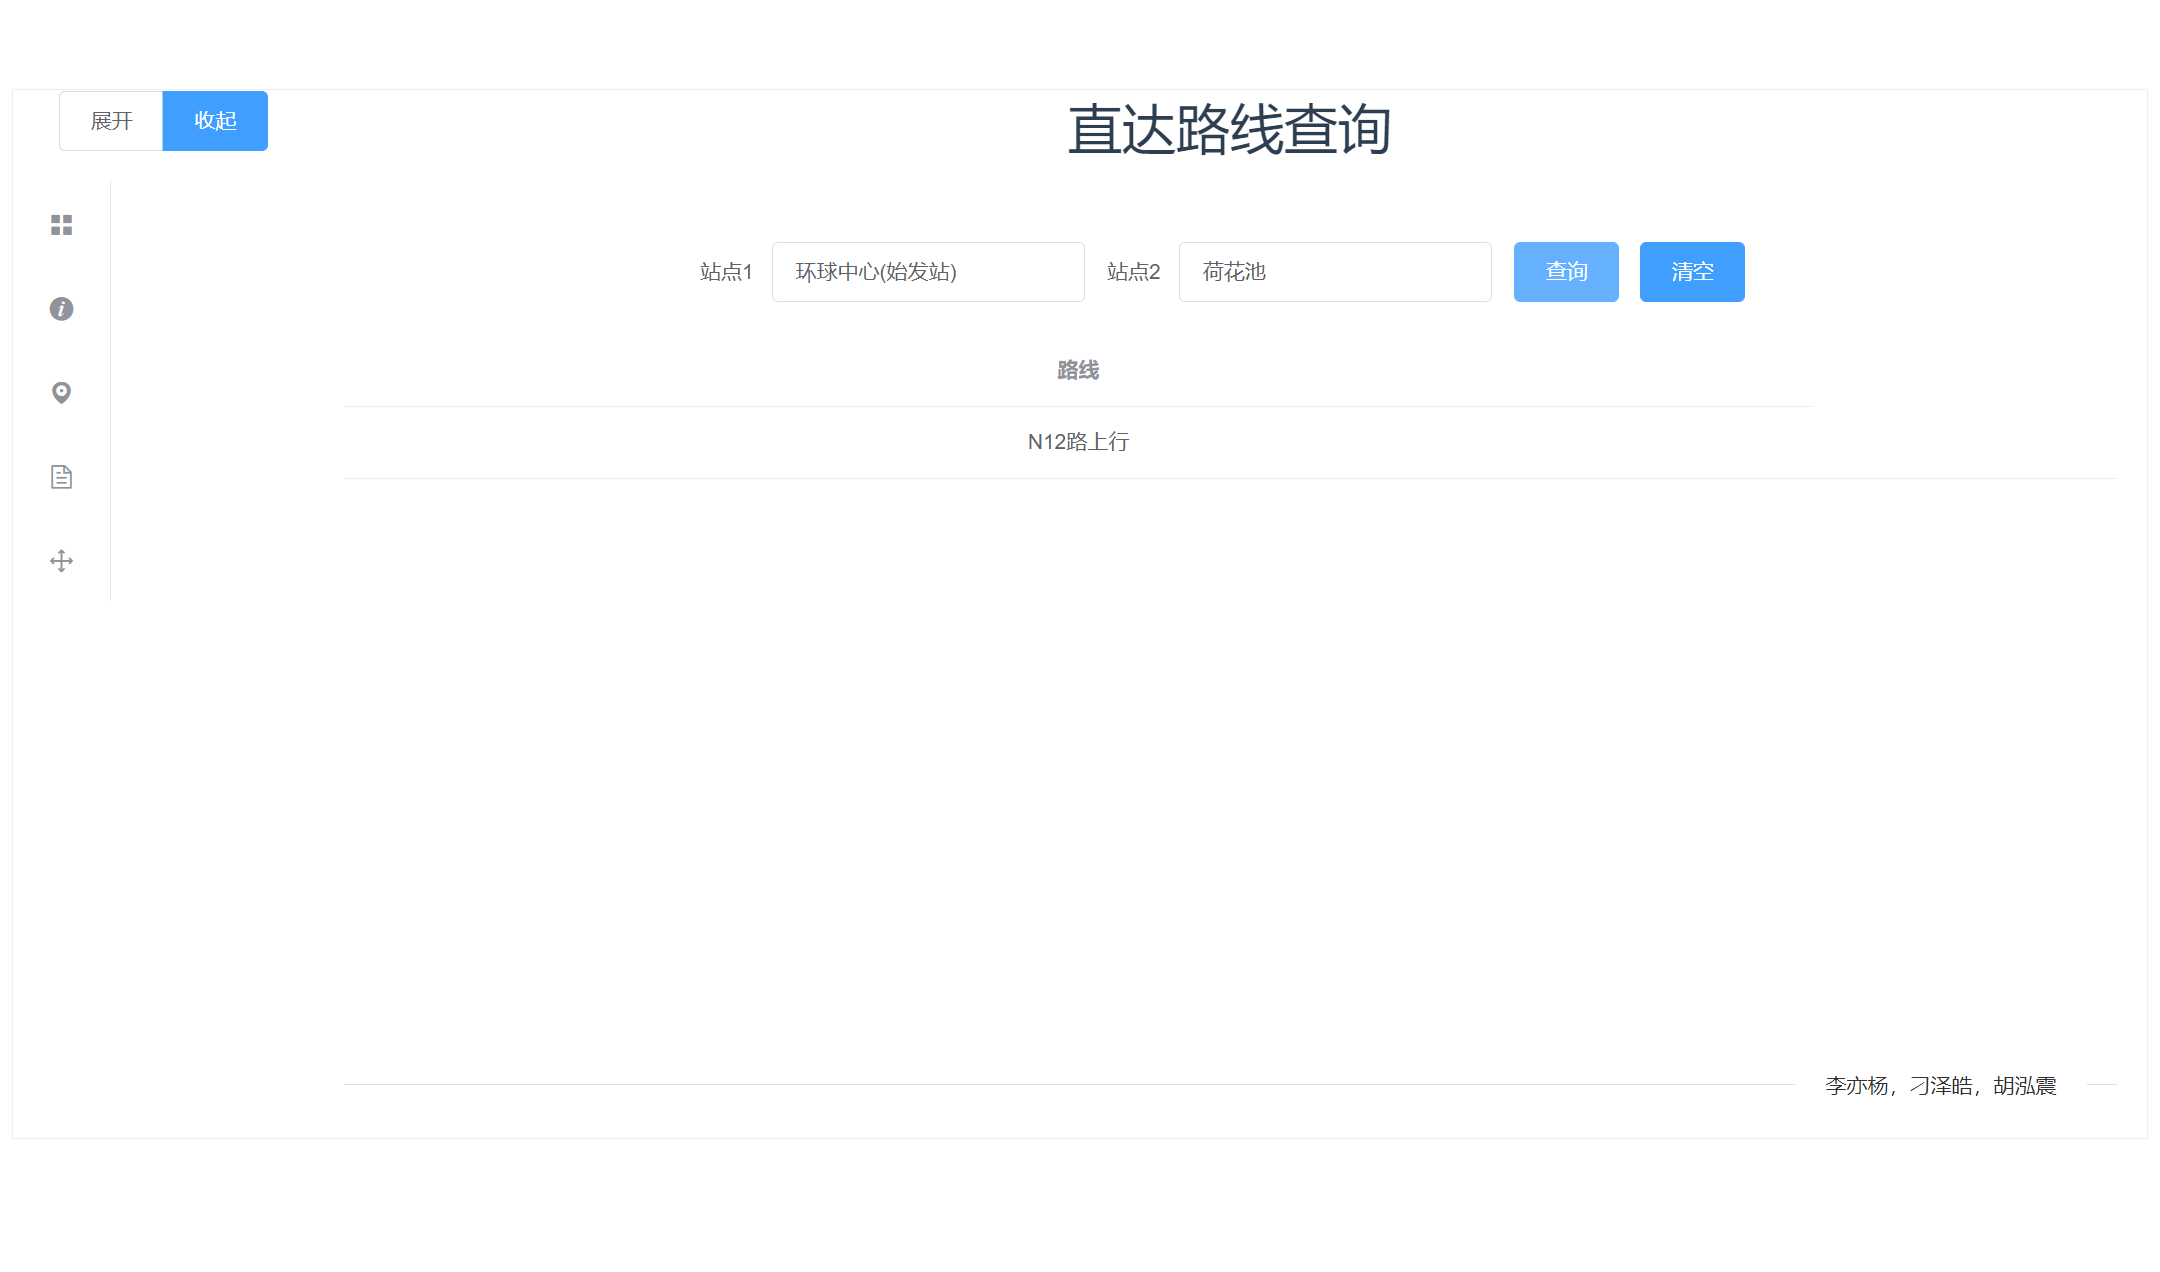
\includegraphics[scale=0.3]{./assets/demand6_1.png} \\ 
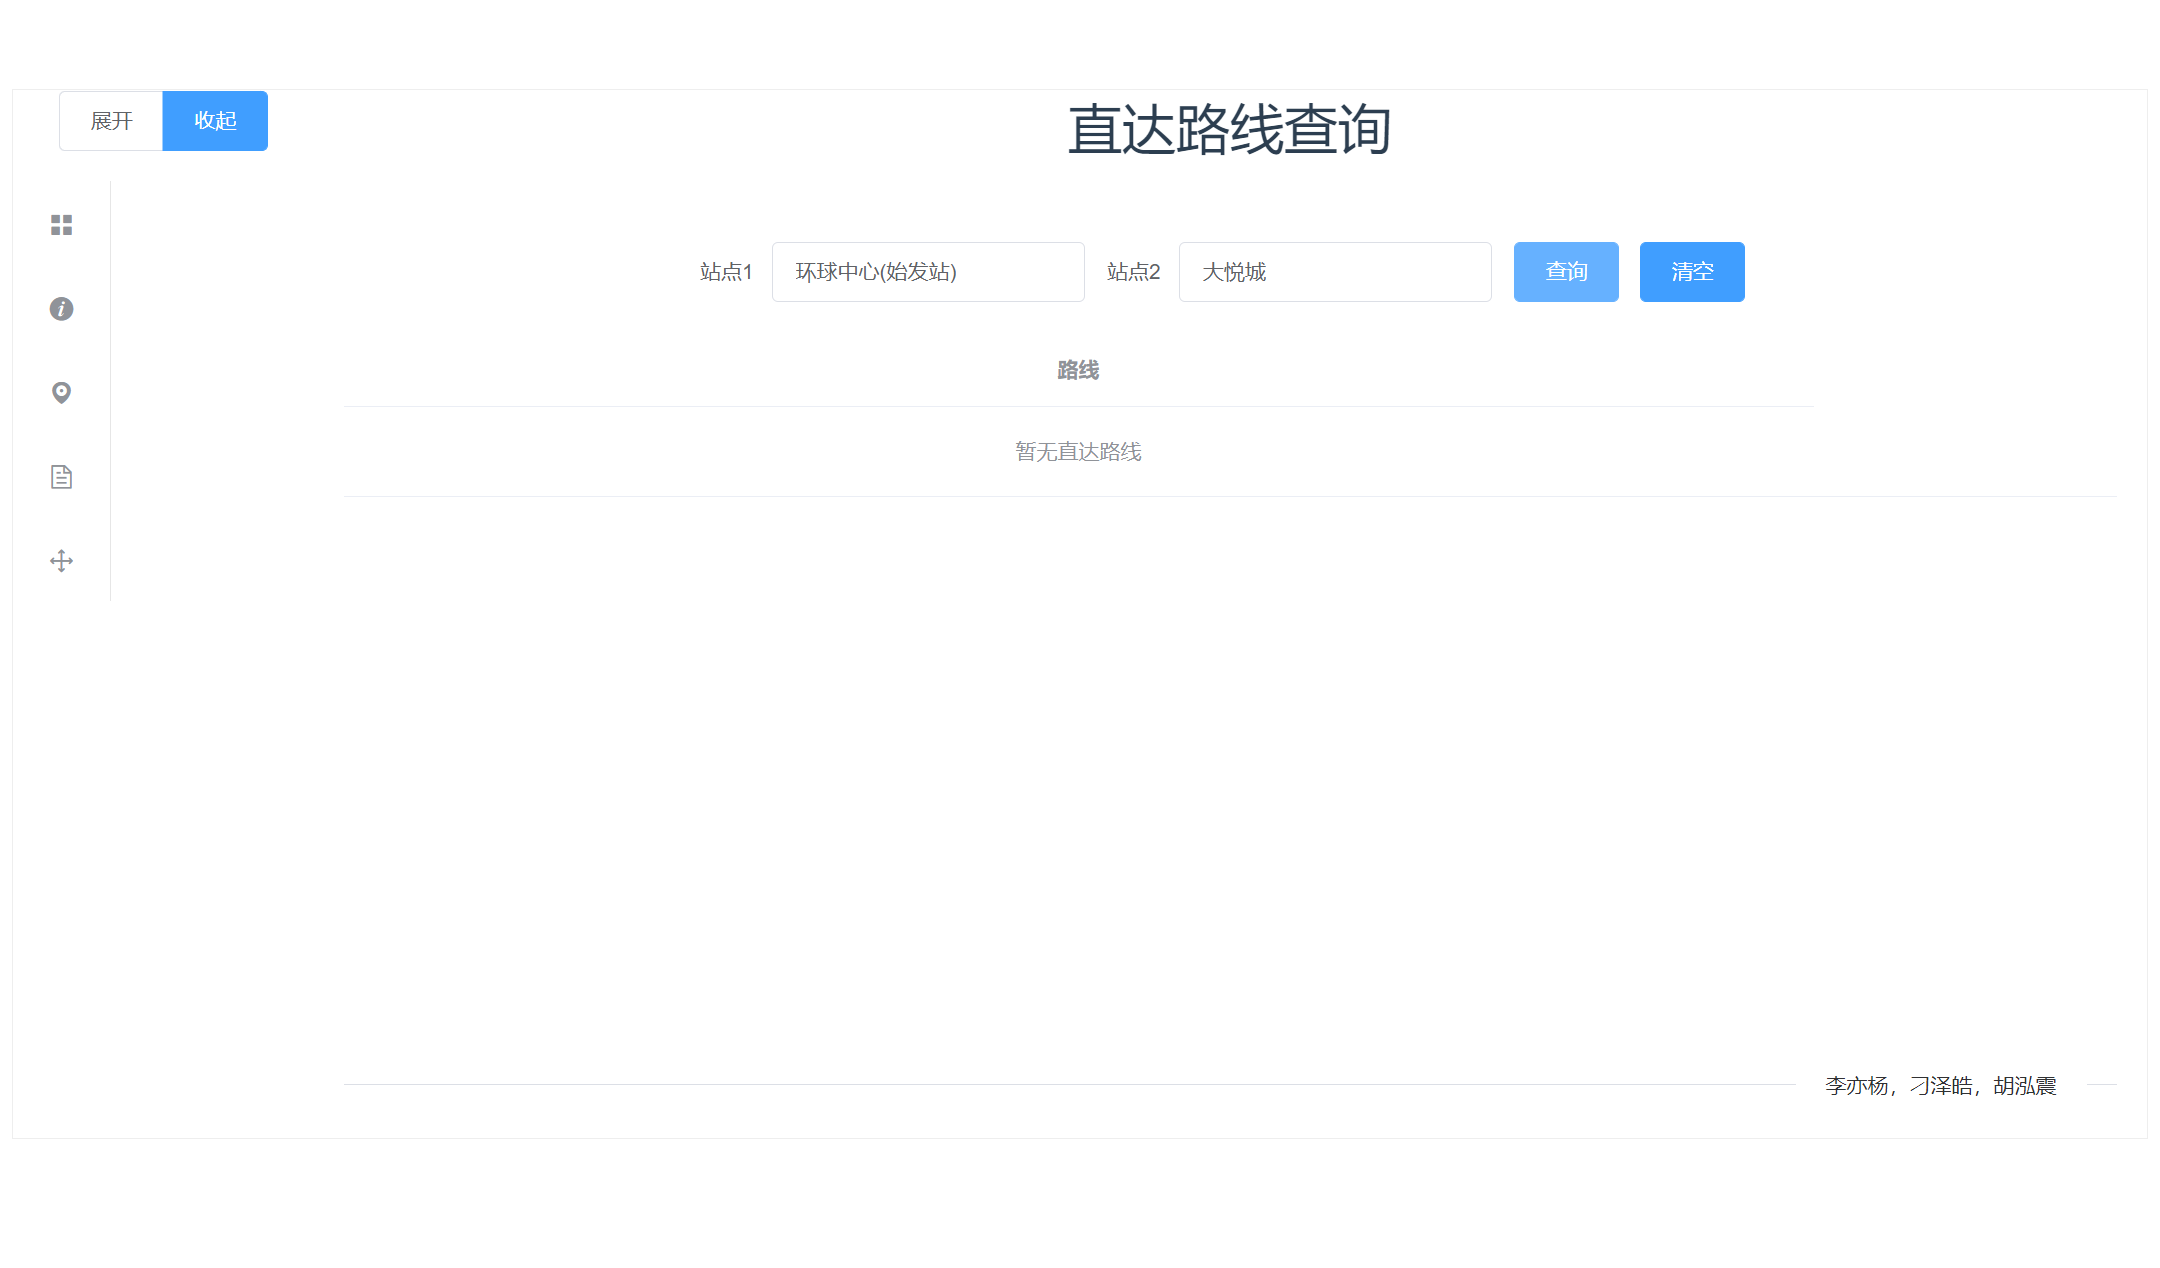
\includegraphics[scale=0.3]{./assets/demand6_2.png} 
\end{center}

\subsection{需求10}
\textbf{统计停靠线路最多的站点前15位,结果显示为4列:站点id,站点名,线路条数,线路名称。} \\
\textbf{Cypher} \\
\begin{lstlisting}[numbers = left, 
showstringspaces=false,
showspaces = false,
breaklines = true, 
language=Java]
@Query("""
	match
		(l:Line) where {station_id} in l.route
	return l.name + l.direction
	""")
ArrayList<String> get_lines_in_a_station(String station_id);
\end{lstlisting} 
第一个函数简单返回所有的站ID。 \\
第二个函数简单返回所有经过该站的线路。

\textbf{业务层} \\
\begin{lstlisting}[numbers = left, 
showstringspaces=false,
showspaces = false,
breaklines = true, 
language=Java]
    public JSONArray most_line_station(){
        JSONArray arr = new JSONArray();
        ArrayList<String> stations;
        stations = stationrepository.get_all_station_id();
        ArrayList<StationLines> sta_lin = new ArrayList<>();
        for(int i = 0;i < stations.size();i++)
        {
            StationLines a = new StationLines();
            a.stationId = stations.get(i);
            a.station = stationrepository.get_station_name_by_id(a.stationId);
            ArrayList<String> line_f;
            line_f = linerepository.get_lines_in_a_station(a.stationId);

            ArrayList<String> line = new ArrayList<>();

            if(!line_f.isEmpty()){
               for(int k = 0; k < line_f.size(); k ++){
                   String tmp = line_f.get(k);
                   if(tmp.contains("up"))
                       tmp = tmp.replace("up", "路上行");
                   else if(tmp.contains("down"))
                       tmp = tmp.replace("down", "路下行");
                   else if(tmp.contains("circle"))
                       tmp = tmp.replace("circle", "路环线");

                   line.add(tmp);
               }
            }

            String s = "";
            if(!line.isEmpty()){
                for(int j = 0;j<line.size();j++)
                {
                    s += line.get(j);
                    if(j < line.size() - 1)
                        s+=",";
                }
            }
            a.route = s;
            a.num = line.size();
            sta_lin.add(a);
        }
        Collections.sort(sta_lin,new SortByNum());
        if(!sta_lin.isEmpty()){
            for(int i = 0;i<15;i++)
            {
                JSONObject obj = new JSONObject();
                StationLines a = new StationLines();
                a = sta_lin.get(i);
                obj.put("stationId",a.stationId);
                obj.put("station",a.station);
                obj.put("num",a.num);
                obj.put("route",a.route);
                arr.add(obj);
            }
        }
        return arr;
    }
\end{lstlisting} 
\begin{lstlisting}[numbers = left, 
showstringspaces=false,
showspaces = false,
breaklines = true, 
language=Java]
class SortByNum implements Comparator {
    public int compare(Object o1,Object o2){
        if(((StationLines)o1).num < ((StationLines)o2).num)
            return 1;
        if(((StationLines)o1).num > ((StationLines)o2).num)
            return -1;
        return 0;
    }
}
\end{lstlisting} 
首先建立了一个新类StationLines,里面包含四个属性:String stationId;String station;int num;String route。并初始化一个该类的列表sta$\_$lin,这对应着结果的4个属性。
先调用StationRepository中的get$\_$all$\_$station$\_$id(),返回所有站点id的列表stations,然后遍历stations,对每个线路id将其加入sta$\_$lin中的stationId属性,然后对每个id调用get$\_$station$\_$name$\_$by$\_$id得到stationName,将其加入sta$\_$lin的station属性,再调用get$\_$lines$\_$in$\_$a$\_$station函数得到经过该站点的线路名的列表,将其变为字符串后加入sta$\_$lin的route属性,将其元素个数加入num属性。
然后调用StationLines的排序类对其按num属性排序,随后转为JSONArray对象输出。

\textbf{前端界面测试结果} \\
\begin{center}
\centering
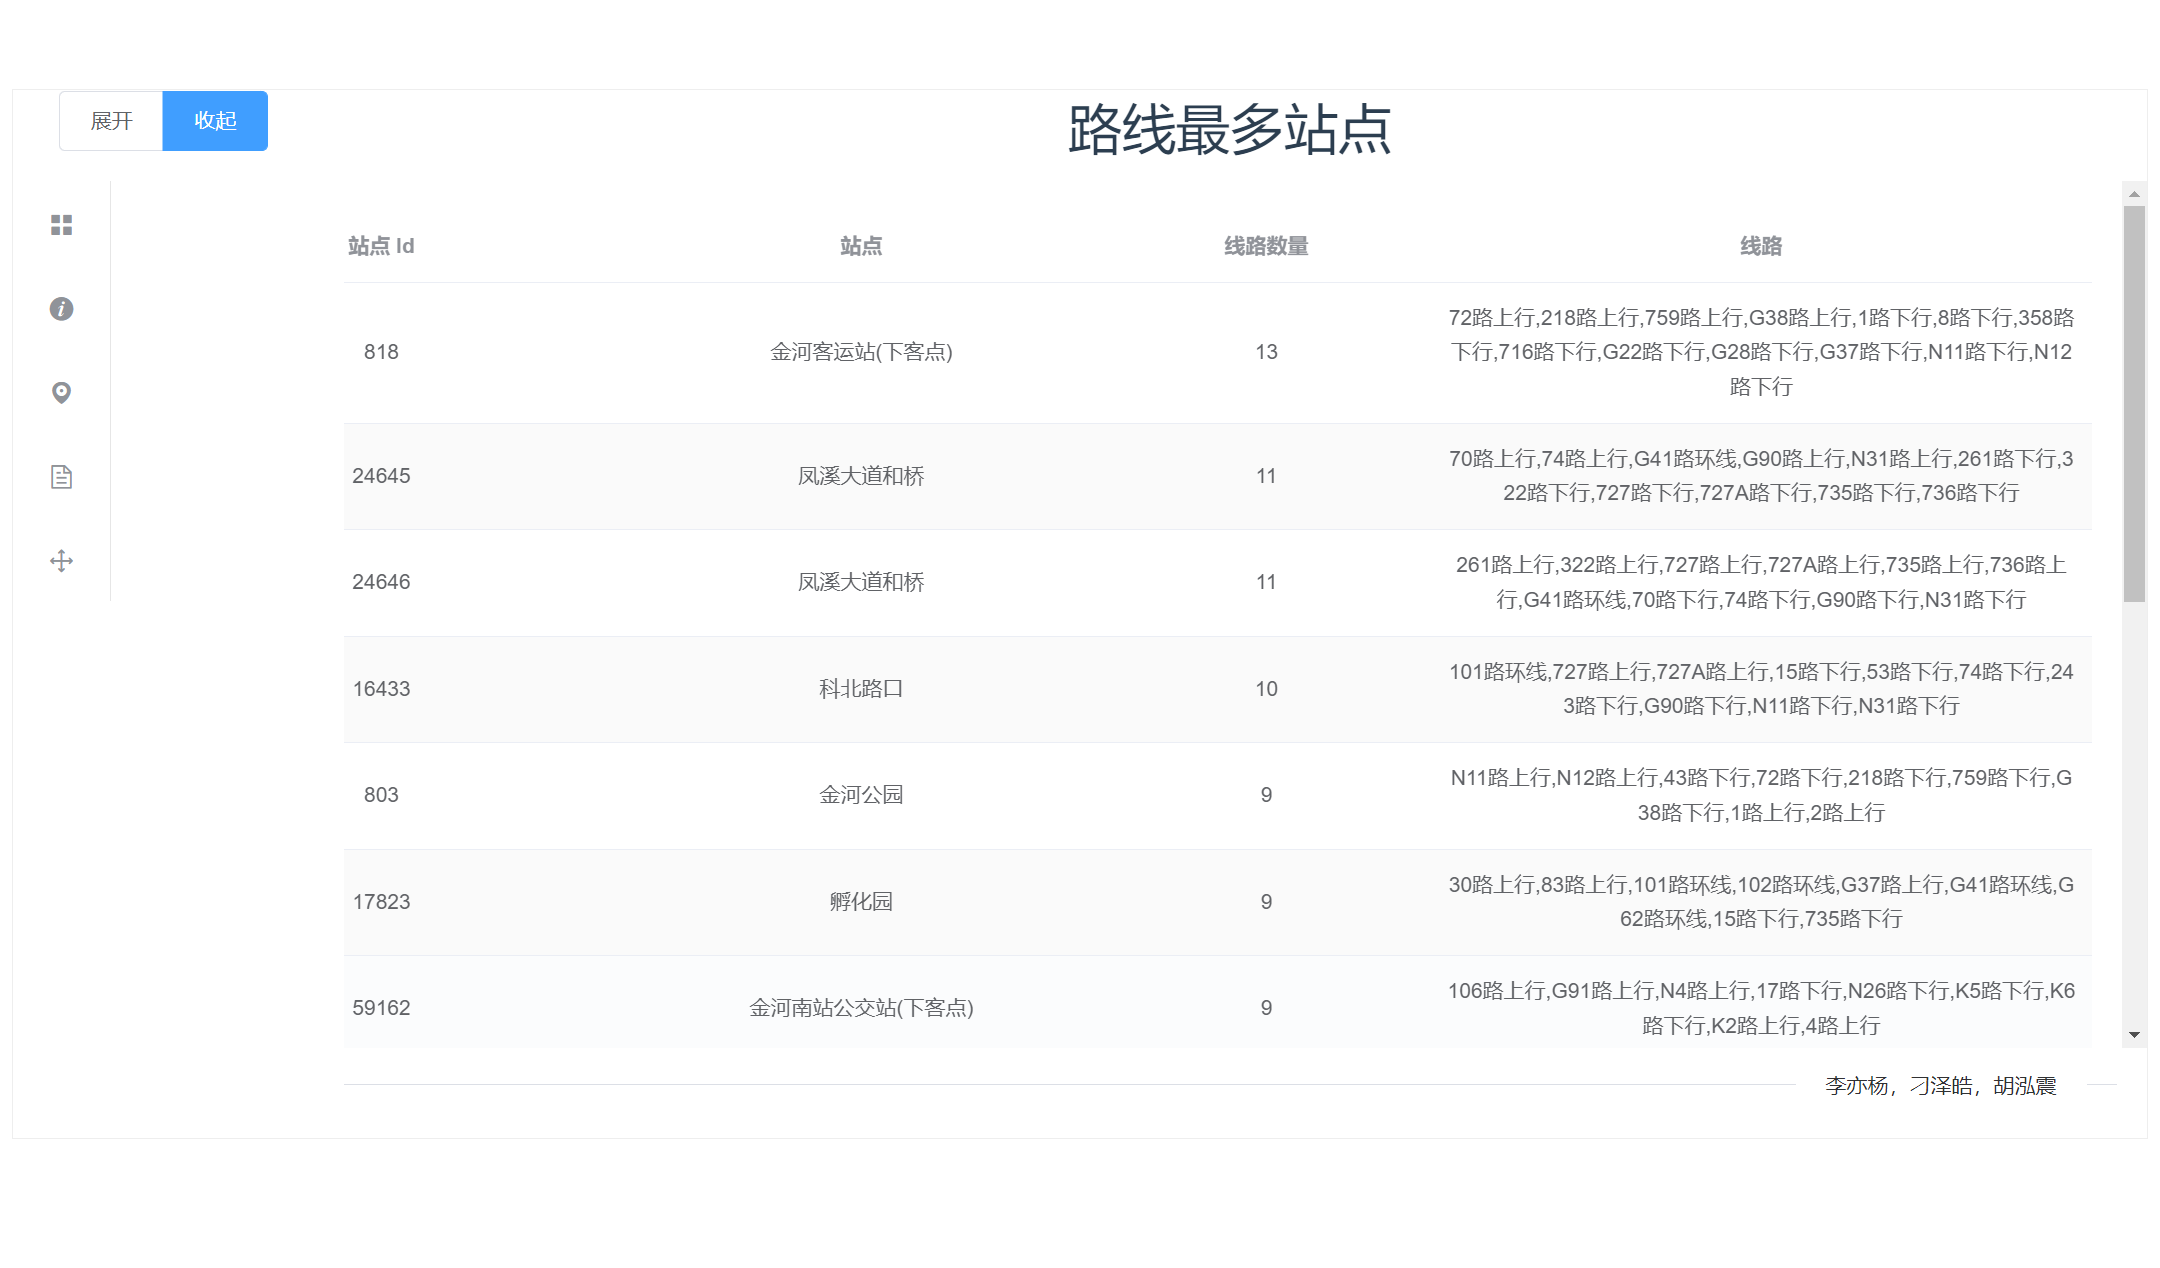
\includegraphics[scale=0.3]{./assets/demand10_1.png} \\ 
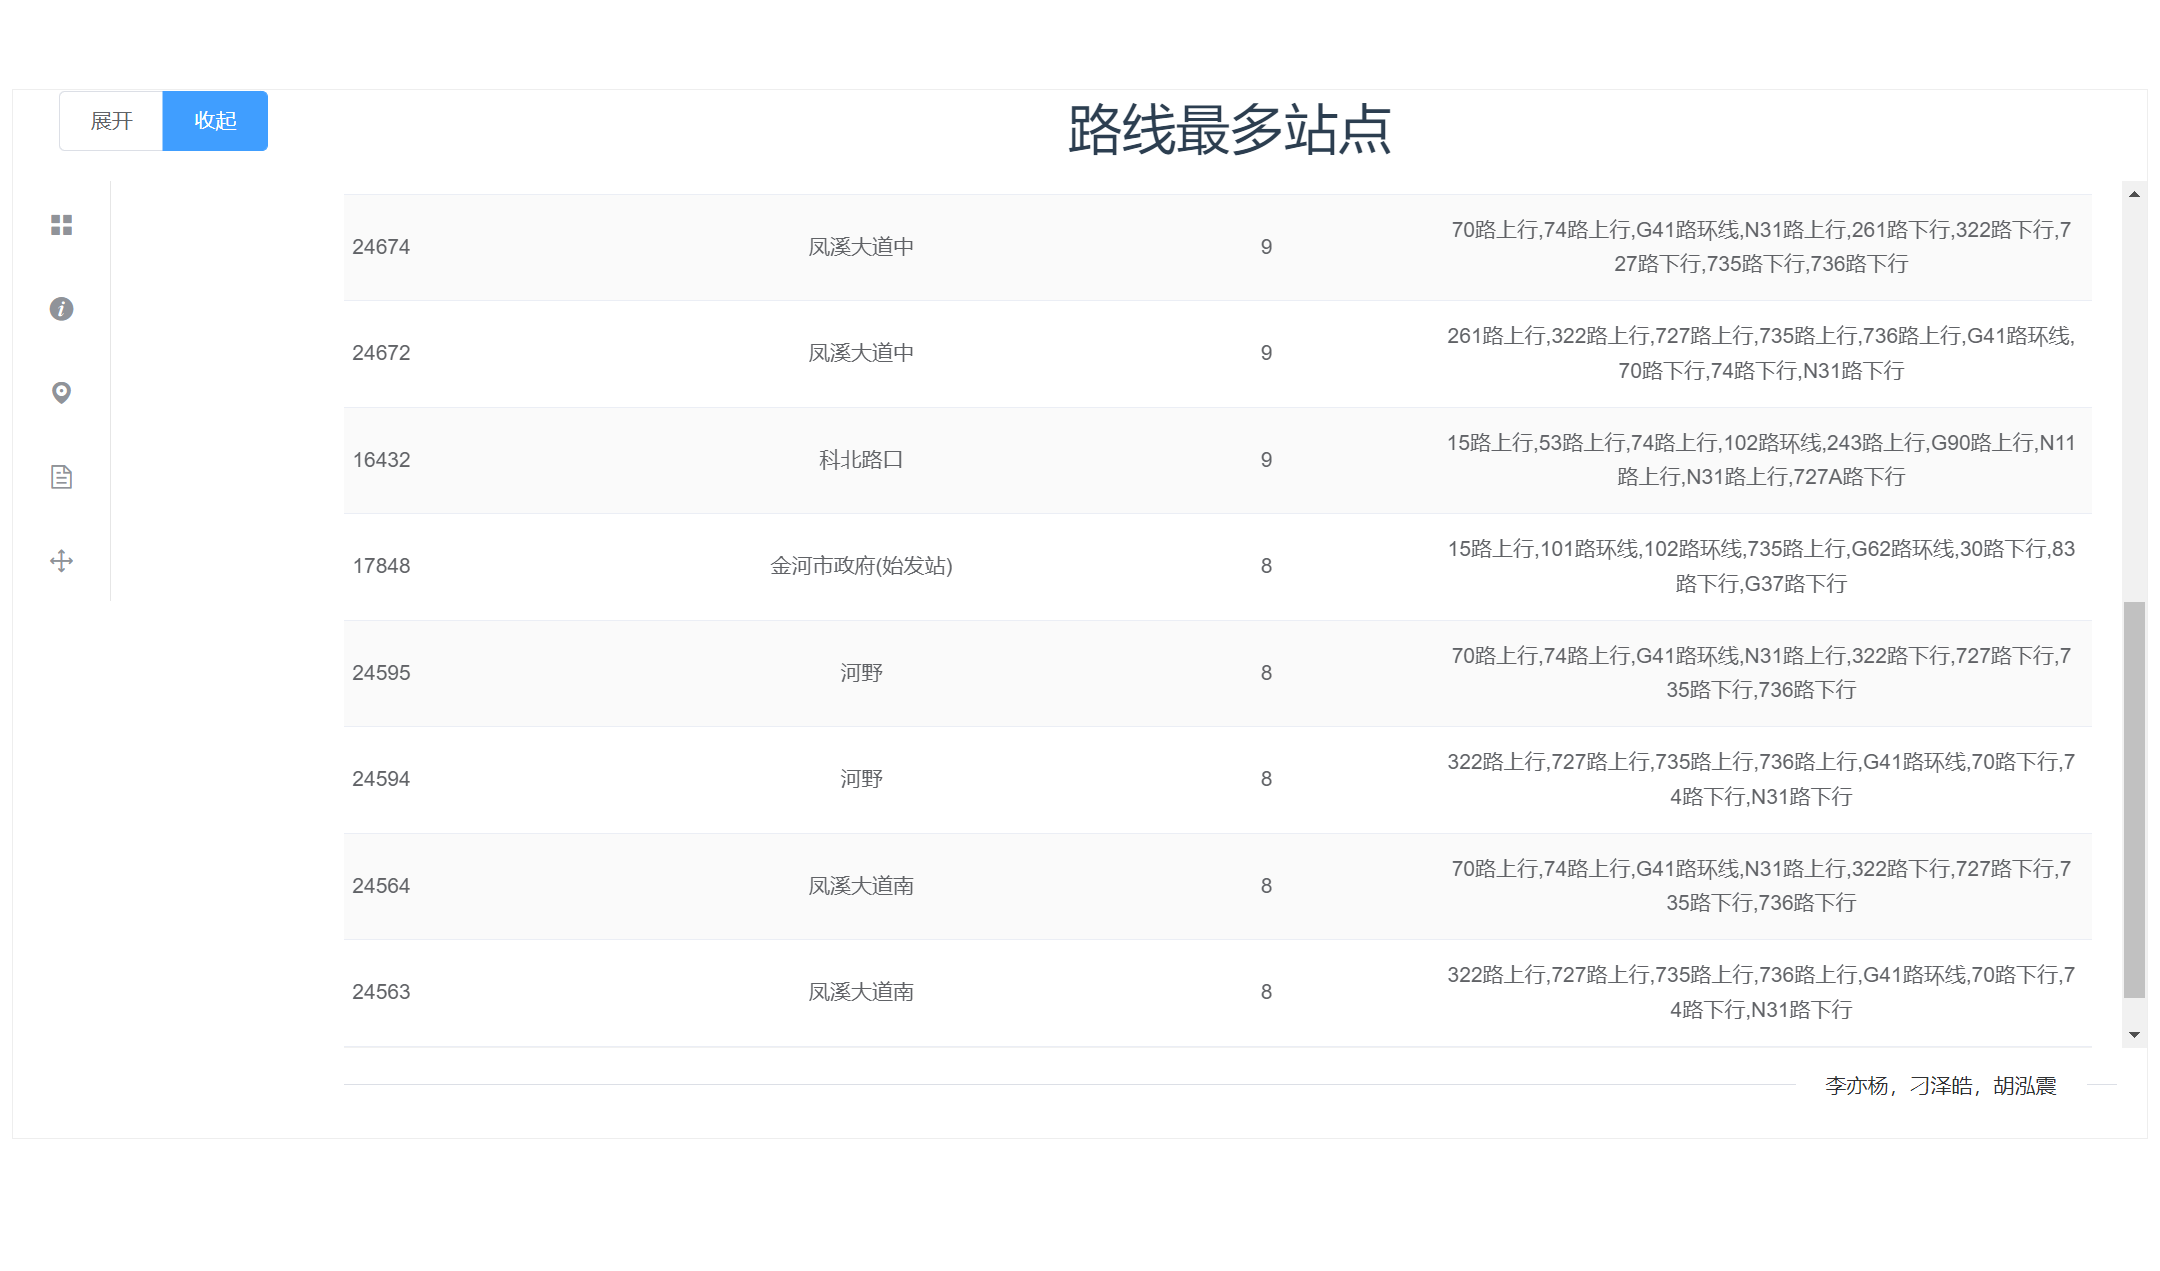
\includegraphics[scale=0.3]{./assets/demand10_2.png} 
\end{center}


\subsection{需求11}
\subsubsection{a}
\textbf{统计地铁站、起点站、终点站数量,并返回站点名。} \\
\textbf{Cypher} \\
\begin{lstlisting}[numbers = left, 
showstringspaces=false,
showspaces = false,
breaklines = true, 
language=Java]
@Query("""
	match (s:Station) where s.name starts with "地铁"
	return distinct s.name
	""")
ArrayList<String> count_subway_station();

@Query("""
	match (s:Station) where s.name ends with "(始发站)" or not () --> (s)
	return distinct s.name
	""")
ArrayList<String> count_start_station();

@Query("""
	match (s:Station) where s.name ends with "(终点站)" or not (s) --> ()
	return distinct s.name
	""")
ArrayList<String> count_end_station();
\end{lstlisting} 
使用三个类似的cypher语句分别进行查询,利用match with关键字来寻找符号条件的全部站点,并返回其中文名称。

\textbf{业务层} \\
\begin{lstlisting}[numbers = left, 
showstringspaces=false,
showspaces = false,
breaklines = true, 
language=Java]
    public JSONObject special_station(){
        JSONObject obj = new JSONObject();
        ArrayList<String> subway;
        subway = stationrepository.count_subway_station();
        ArrayList<String> start;
        start = stationrepository.count_start_station();
        ArrayList<String> end;
        end = stationrepository.count_end_station();
        if(!subway.isEmpty())
        {
            JSONObject obj1 = new JSONObject();
            obj1.put("type","地铁站");
            obj1.put("amount",subway.size());
            JSONArray arr =new JSONArray();
            String s = "";
            for(int i =0;i<subway.size();i++)
            {
                JSONObject t = new JSONObject();
                s = subway.get(i);
                t.put("station", s);
                arr.add(t);
            }
            obj1.put("stations",arr);
            obj.put("subway",obj1);
        }
        if(!start.isEmpty())
        {
            JSONObject obj1 = new JSONObject();
            obj1.put("type","始发站");
            obj1.put("amount",start.size());
            JSONArray arr =new JSONArray();
            String s = "";
            for(int i =0;i<start.size();i++)
            {
                JSONObject t = new JSONObject();
                s = start.get(i);
                t.put("station", s);
                arr.add(t);
            }
            obj1.put("stations",arr);
            obj.put("start",obj1);
        }
        if(!end.isEmpty())
        {
            JSONObject obj1 = new JSONObject();
            obj1.put("type","终点站");
            obj1.put("amount",end.size());
            JSONArray arr =new JSONArray();
            String s = "";
            for(int i =0;i<end.size();i++)
            {
                JSONObject t = new JSONObject();
                s = end.get(i);
                t.put("station", s);
                arr.add(t);
            }
            obj1.put("stations",arr);
            obj.put("end",obj1);
        }

        return obj;
    }
\end{lstlisting} 
直接调用dao层上述三个函数即可。\\
为了确保前端界面的美观程度,将地铁站、始发站和终点站分别整合为一个JSON对象,并将这三个JSON对象整合为一个JSON对象返回。

\textbf{前端界面测试结果} \\
\begin{center}
\centering
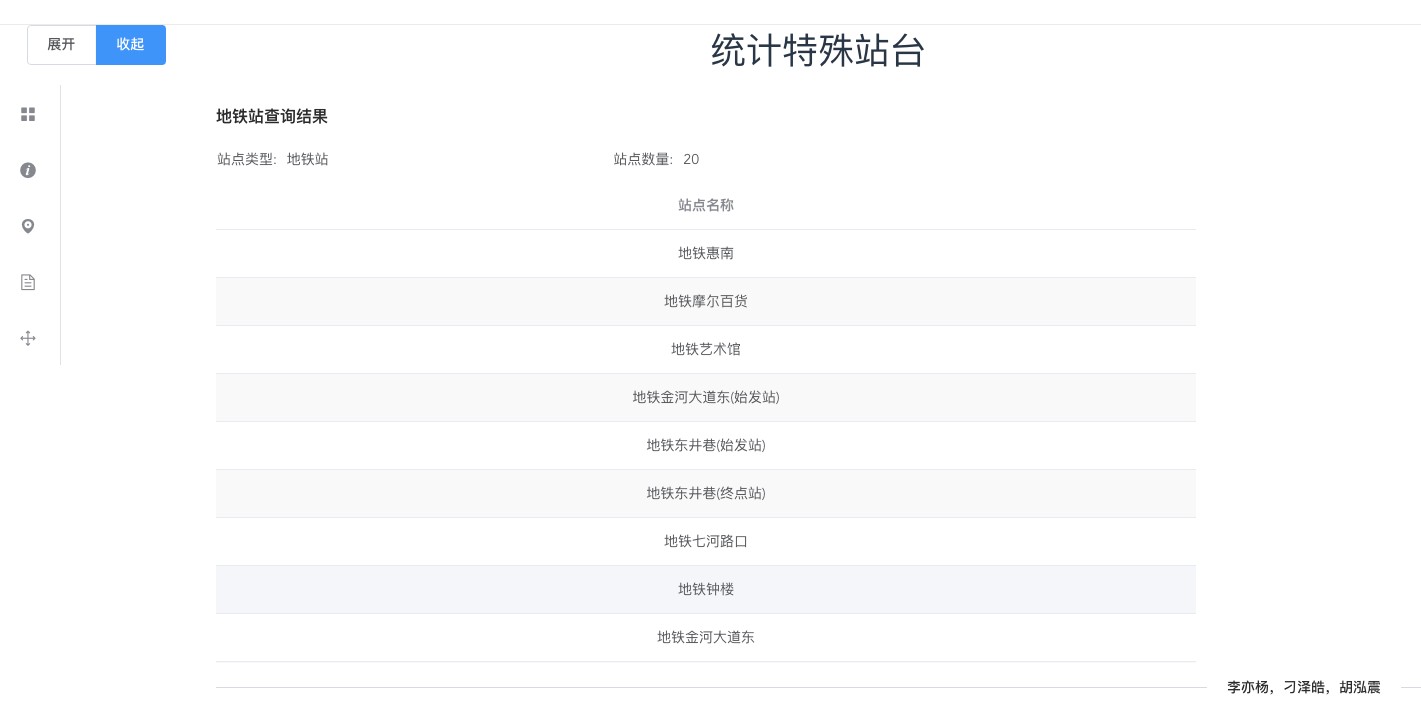
\includegraphics[scale=0.3]{./assets/demand11_1.png} \\ 
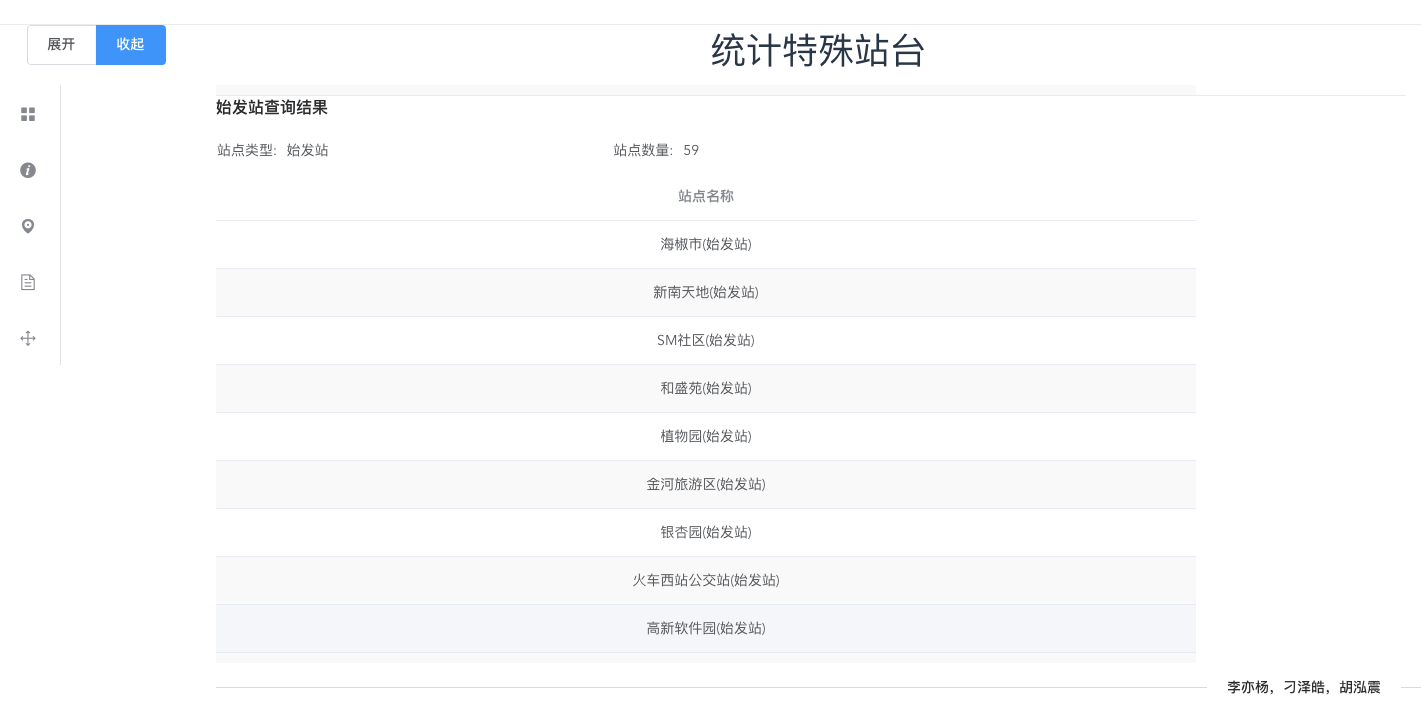
\includegraphics[scale=0.3]{./assets/demand11_2.png} \\ 
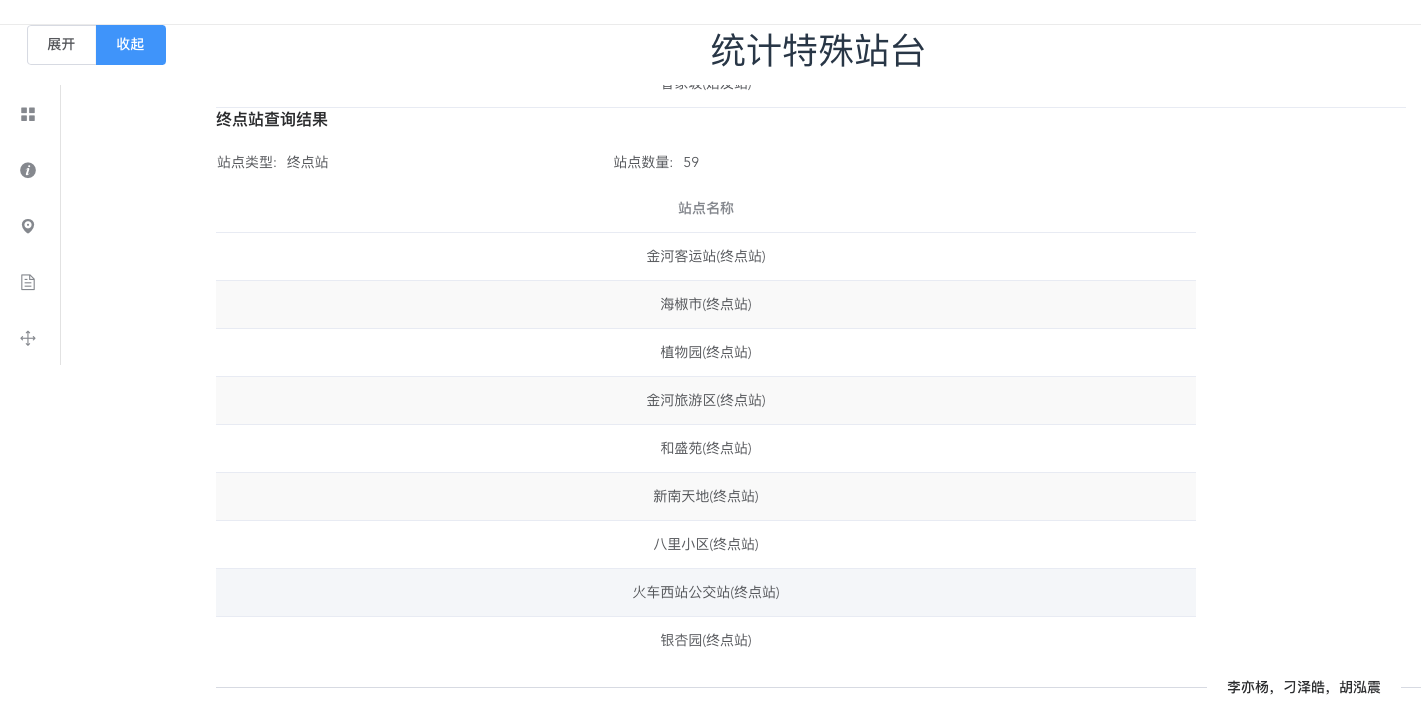
\includegraphics[scale=0.3]{./assets/demand11_3.png} 
\end{center}


\subsection{需求12}
\textbf{分组统计常规公交(包括干线、支线、城乡线、驳接线、社区线)、 快速公交(K字开头)、高峰公交(G字开头)、夜班公交(N字开头)。返回四类名称及对应数量。} \\
\textbf{Cypher} \\
\begin{lstlisting}[numbers = left, 
showstringspaces=false,
showspaces = false,
breaklines = true, 
language=Java]
@Query("""
	match (l:Line) where l.name =~ "^[0-9]+"
	return count(l)
	""")
Integer count_type_l();

@Query("""
	match (k:Line) where k.name starts with "K"
	return count(k)
	""")
Integer count_type_k();

@Query("""
	match (g:Line) where g.name starts with "G"
	return count(g)
	""")
Integer count_type_g();

@Query("""
	match (n:Line) where n.name starts with "N"
	return count(n)
	""")
Integer count_type_n();
\end{lstlisting} 
每个函数利用正则匹配对应类型站点名,然后返回匹配的站数。

\textbf{业务层} \\
\begin{lstlisting}[numbers = left, 
showstringspaces=false,
showspaces = false,
breaklines = true, 
language=Java]
    public JSONArray count_type(){
        JSONArray arr = new JSONArray();
        int[] count = new int[4];
        count[0] = linerepository.count_type_l();
        count[1] = linerepository.count_type_k();
        count[2] = linerepository.count_type_g();
        count[3] = linerepository.count_type_n();
        ArrayList<String> type = new ArrayList<>();
        type.add("常规公交");
        type.add("快速公交");
        type.add("高峰公交");
        type.add("夜班公交");
        for(int i = 0 ; i < 4; i++)
        {
            JSONObject obj = new JSONObject();
            int a = count[i];
            obj.put("type",type.get(i));
            obj.put("num",a);
            arr.add(obj);
        }
        return arr;
    }
\end{lstlisting} 
分别调用count$\_$type$\_$l,count$\_$type$\_$k,count$\_$type$\_$g,count$\_$type$\_$n四个函数返回四种线路类型的数量,然后将其整合为JSONArray对象返回。 \\
事实上,原本设想通过建立Demand系列里虚构类来对非实体对象进行抽象,从而便于通过同一条Cypher语句来返回获得的数据,然而由于使用的SDN6移除了@QueryMapper等命令,而选择通过Neo4jDriver与Driver的形式来完成了Query与非实体类之间的映射的实现,考虑到可能用到的非实体类较少,且该种形式过于复杂,因而我们选择了拆分Query查询语句的方式进行实现。之后需求倘若有涉及到Demand类的使用的,在数据库查询层面都利用拆分的方式进行了实现。

\textbf{前端界面测试结果} \\
\begin{center}
\centering
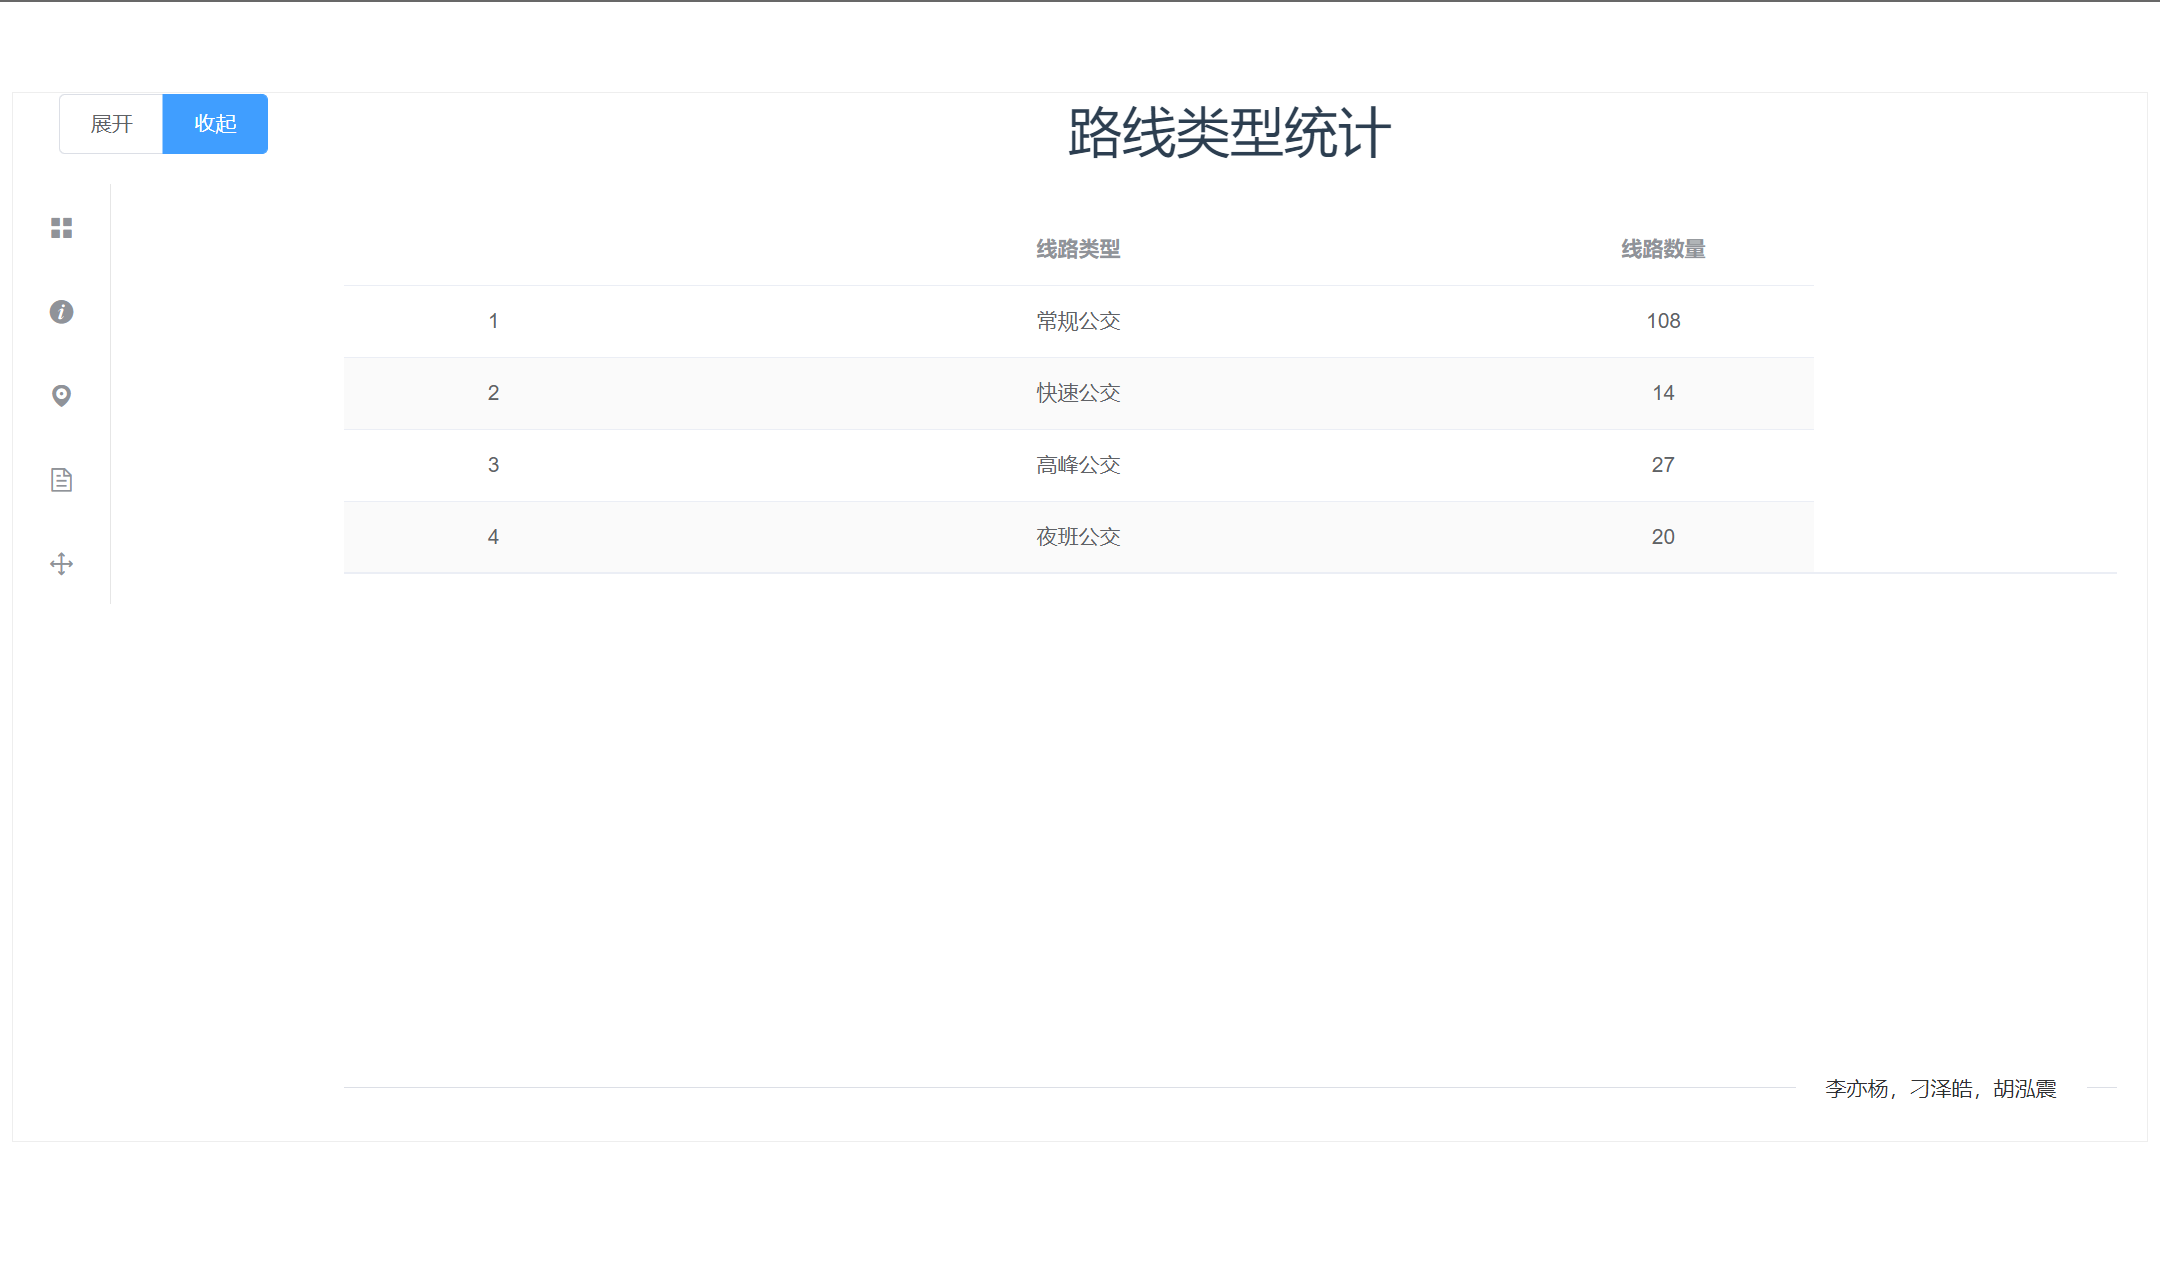
\includegraphics[scale=0.3]{./assets/demand12.png} 
\end{center}

\subsection{需求13}
\textbf{查询两条线路重复的站点名,返回相同站点的id,名称、英文名。} \\
\textbf{Cypher} \\
由Service层调用find$\_$route$\_$station两次。

\textbf{业务层} \\
\begin{lstlisting}[numbers = left, 
showstringspaces=false,
showspaces = false,
breaklines = true, 
language=Java]
    public JSONArray find_sameStations(String id1,String direction1,String id2,String direction2){
        JSONArray arr = new JSONArray();
        ArrayList<Station> result1;
        result1 = stationrepository.find_route_station(id1,direction1);
        ArrayList<Station> result2;
        result2 = stationrepository.find_route_station(id2,direction2);
        Station sta;
        //result1.retainAll(result2);



        ArrayList<Station> to_delete = new ArrayList<>();
        if(!result1.isEmpty()){
            for(int i = 0; i < result1.size(); i ++){
                boolean has = false;
                if(!result2.isEmpty()){
                    for(int j = 0; j < result2.size(); j ++){
                        if(Objects.equals(result1.get(i).getId(), result2.get(j).getId())){
                            has = true;
                            break;
                        }
                    }
                }
                if(!has){
                    to_delete.add(result1.get(i));
                }
            }
        }

        for(int i = 0; i < to_delete.size(); i ++)
            result1.remove(to_delete.get(i));

        if(!result1.isEmpty()){
            for(int i = 0 ; i < result1.size() ; i++)
            {
                sta = result1.get(i);
                JSONObject obj = new JSONObject();
                obj.put("station_id",sta.getId());
                obj.put("station_name",sta.getName());
                obj.put("station_english",sta.getEnglish());
                arr.add(obj);
            }
        }
        return arr;
    }
\end{lstlisting} 
对两个线路名分别调用find$\_$route$\_$station函数,返回两个线路对应的站点列表,然后对两个列表求交集,将结果转化为JSONArray对象返回。


\textbf{前端界面测试结果} \\
\begin{center}
\centering
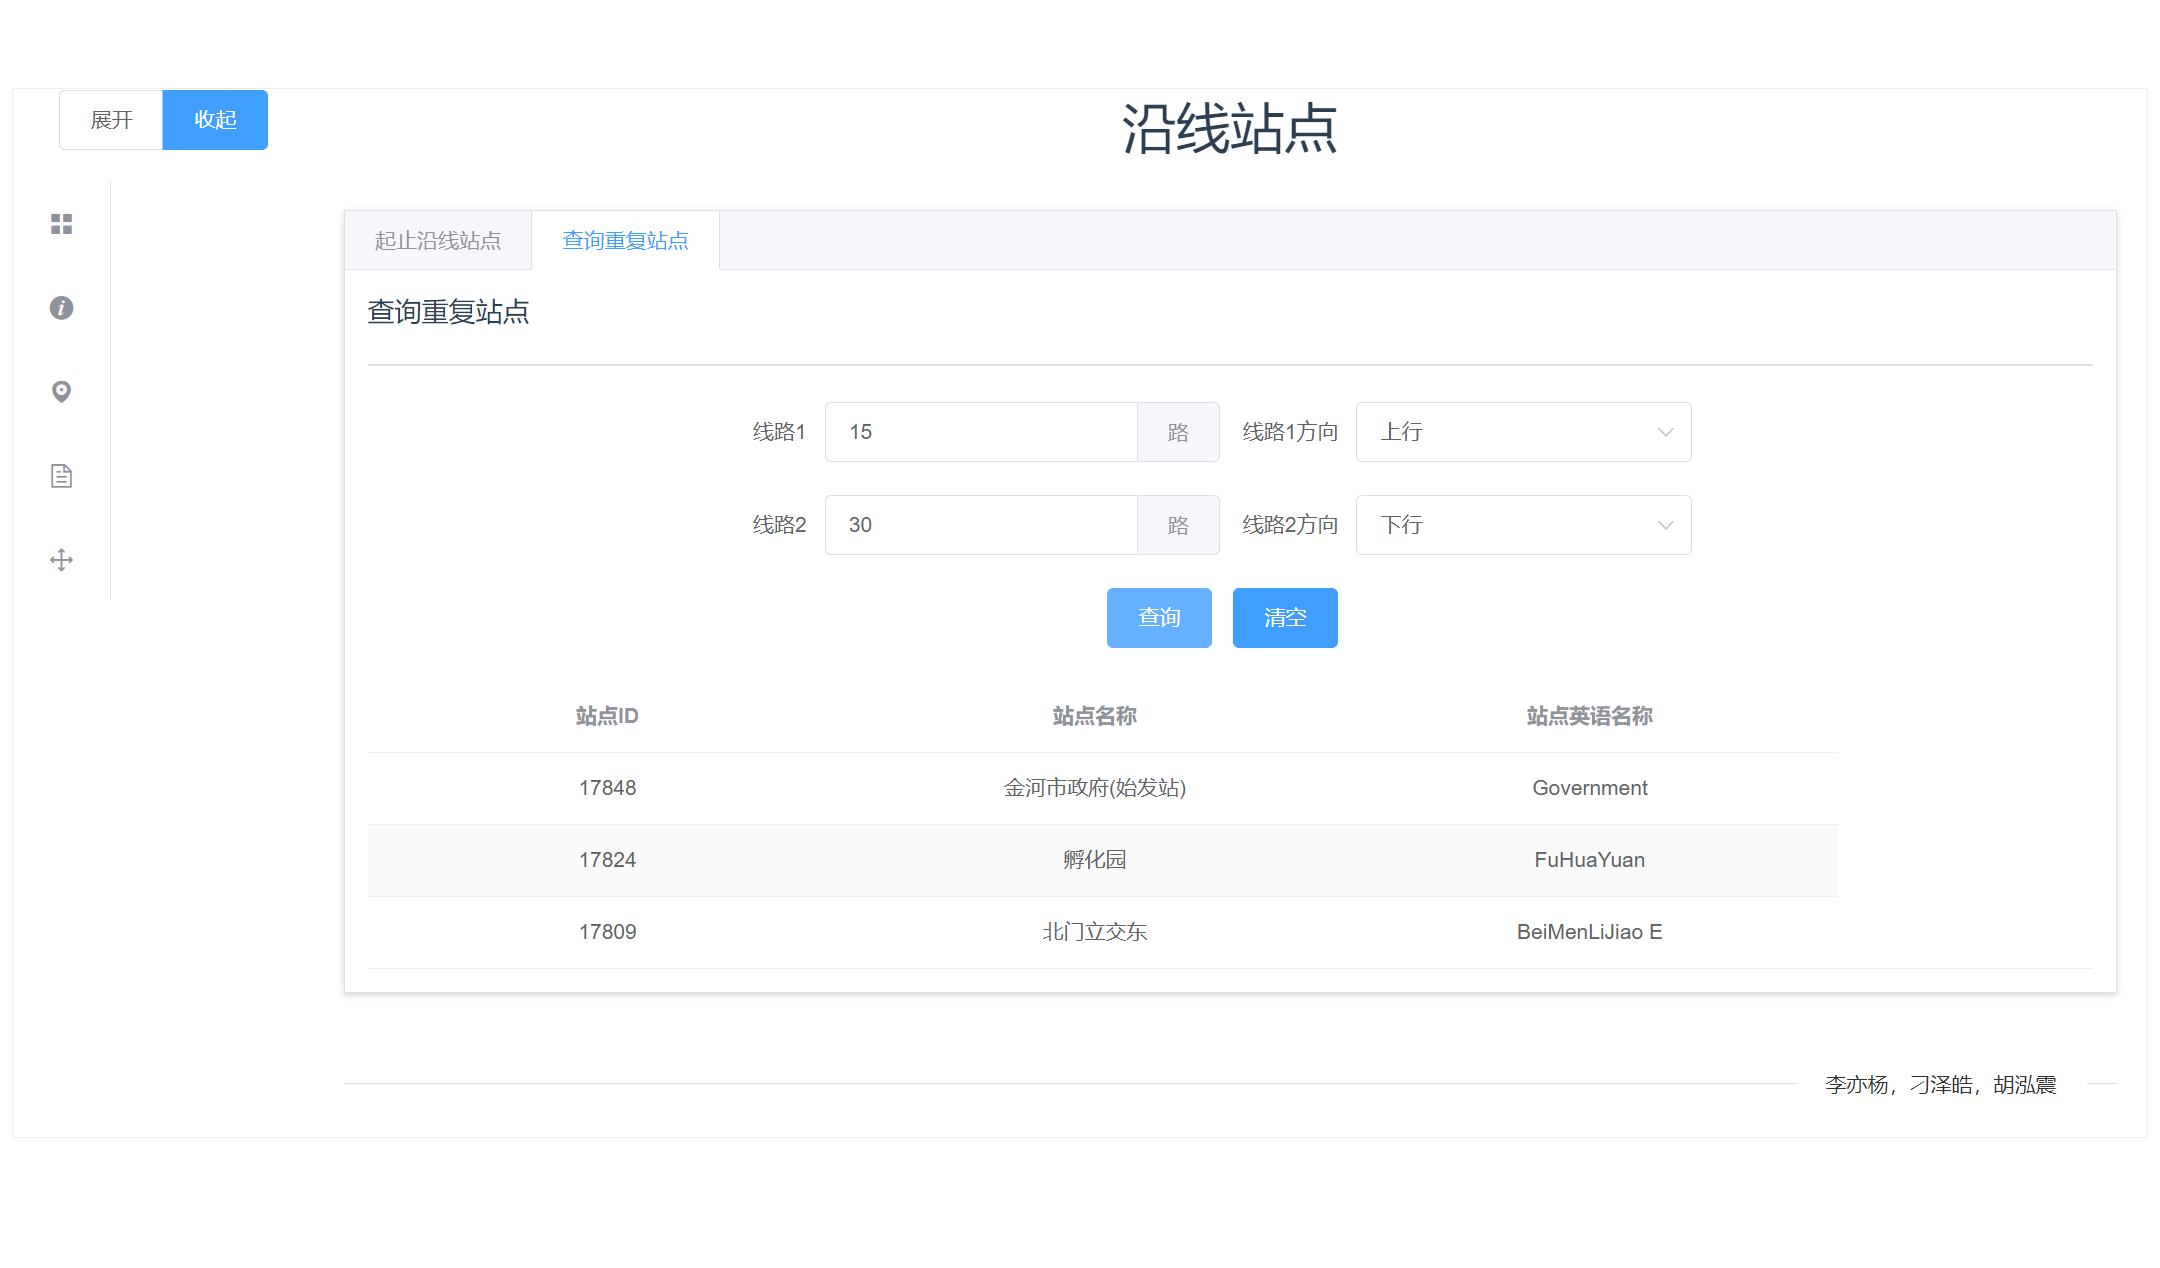
\includegraphics[scale=0.3]{./assets/demand13_1.png} \\ 
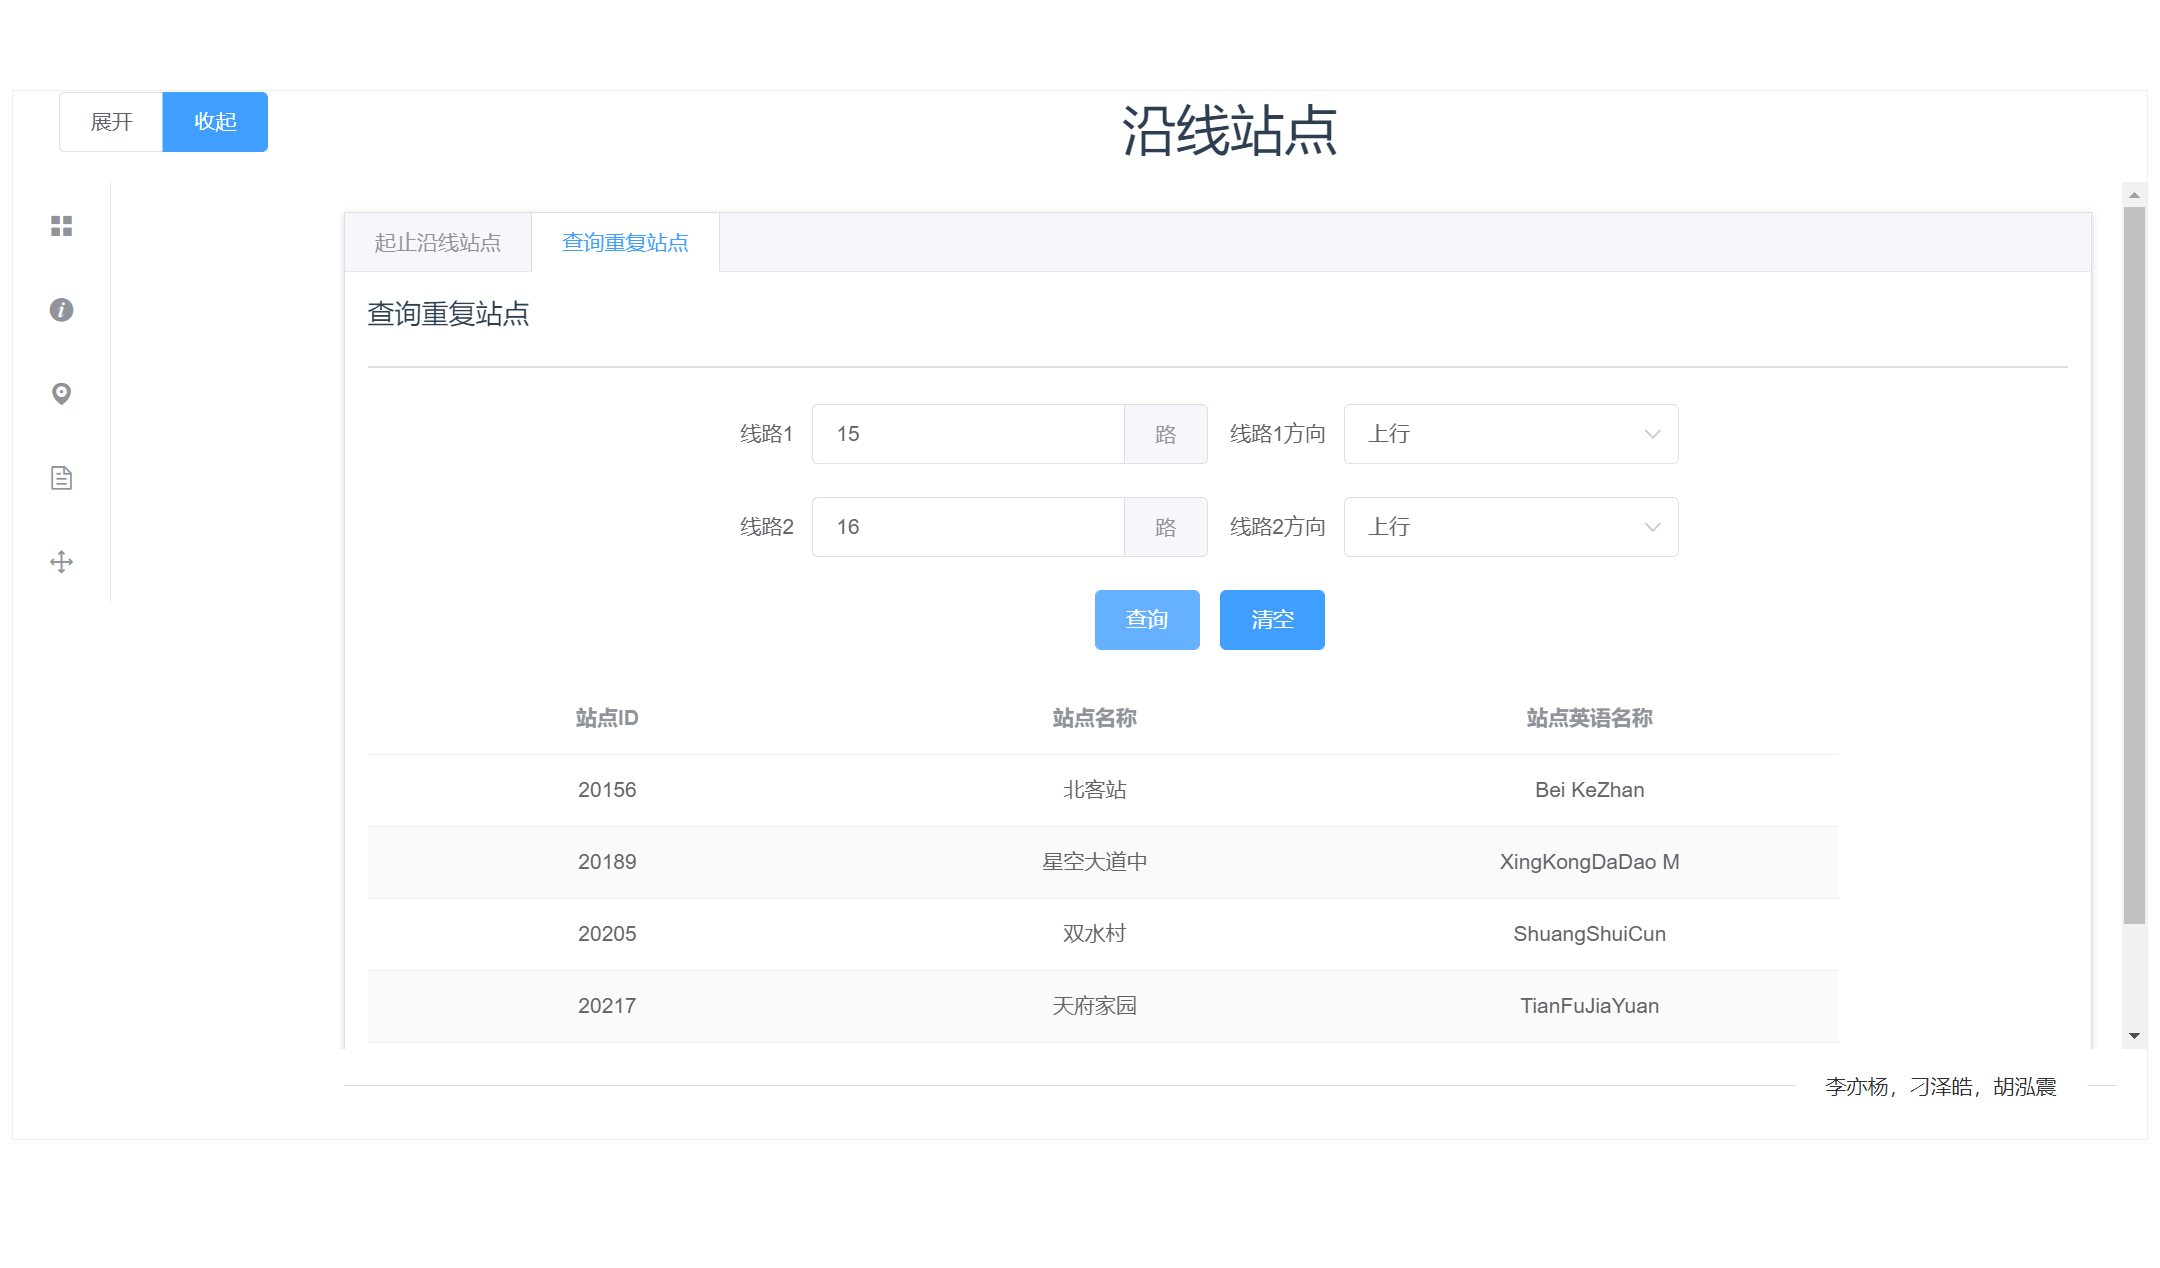
\includegraphics[scale=0.3]{./assets/demand13_2.png} 
\end{center}

\subsection{需求15}
\textbf{查询两个相邻站点间线路数量并排序,输出连接数量排序前15的两站台名和对应线路数量(考虑方向性)。} \\
\textbf{Cypher} \\
\begin{lstlisting}[numbers = left, 
showstringspaces=false,
showspaces = false,
breaklines = true, 
language=Java]
@Query("""
	match(a:Station) -[r]-> (b:Station)
	with a, b, length(r.lines) as cnt
	order by cnt desc
	return a.name limit 15
	""")
ArrayList<String> most_connection_in();

@Query("""
	match(a:Station) -[r]-> (b:Station)
	with a, b, length(r.lines) as cnt
	order by cnt desc
	return b.name limit 15
	""")
ArrayList<String> most_connection_out();

@Query("""
	match(a:Station) -[r]-> (b:Station)
	with a, b, length(r.lines) as cnt
	order by cnt desc
	return cnt limit 15
	""")
ArrayList<Integer> most_connection_count();
\end{lstlisting} 
匹配所有Connection关系,然后根据lines的元素格式降序排序,输出前15个。

\textbf{业务层} \\
\begin{lstlisting}[numbers = left, 
showstringspaces=false,
showspaces = false,
breaklines = true, 
language=Java]
    public JSONArray most_connections(){
        JSONArray arr = new JSONArray();
        ArrayList<String> res_in = stationrepository.most_connection_in();
        ArrayList<String> res_out = stationrepository.most_connection_out();
        ArrayList<Integer> res_cnt = stationrepository.most_connection_count();
        ArrayList<Demand15> result = new ArrayList<>();
        if(!res_cnt.isEmpty()){
            for(int i = 0; i < res_cnt.size(); i++){
                Demand15 dem = new Demand15();
                dem.name_in = res_in.get(i);
                dem.name_out = res_out.get(i);
                dem.count = res_cnt.get(i);
                result.add(dem);
            }

            Collections.sort(result,new SortByCount());
            Demand15 a = new Demand15();

            for(int i = 0 ; i < 15 ;i++)
            {
                a = result.get(i);
                JSONObject obj = new JSONObject();
                obj.put("station1",a.name_in);
                obj.put("station2",a.name_out);
                obj.put("num",a.count);
                arr.add(obj);
            }
        }
        return arr;
    }
\end{lstlisting} 
\begin{lstlisting}[numbers = left, 
showstringspaces=false,
showspaces = false,
breaklines = true, 
language=Java]
public class SortByCount implements Comparator {
    public int compare(Object o1,Object o2){
        if(((Demand15)o1).count < ((Demand15)o2).count)
            return 1;
        if(((Demand15)o1).count > ((Demand15)o2).count)
            return -1;
        return 0;
    }
}
\end{lstlisting} 
分别调用most$\_$connection$\_$in,most$\_$connection$\_$out,most$\_$connection$\_$count函数,返回两个站名列表和一个整数列表,对应每对相邻站点的名字和之间的线路数。将其整合为一个Demand15列表,对其按count属性降序排序,然后将其前15位转为JSONArray对象输出。

\textbf{前端界面测试结果} \\
\begin{center}
\centering
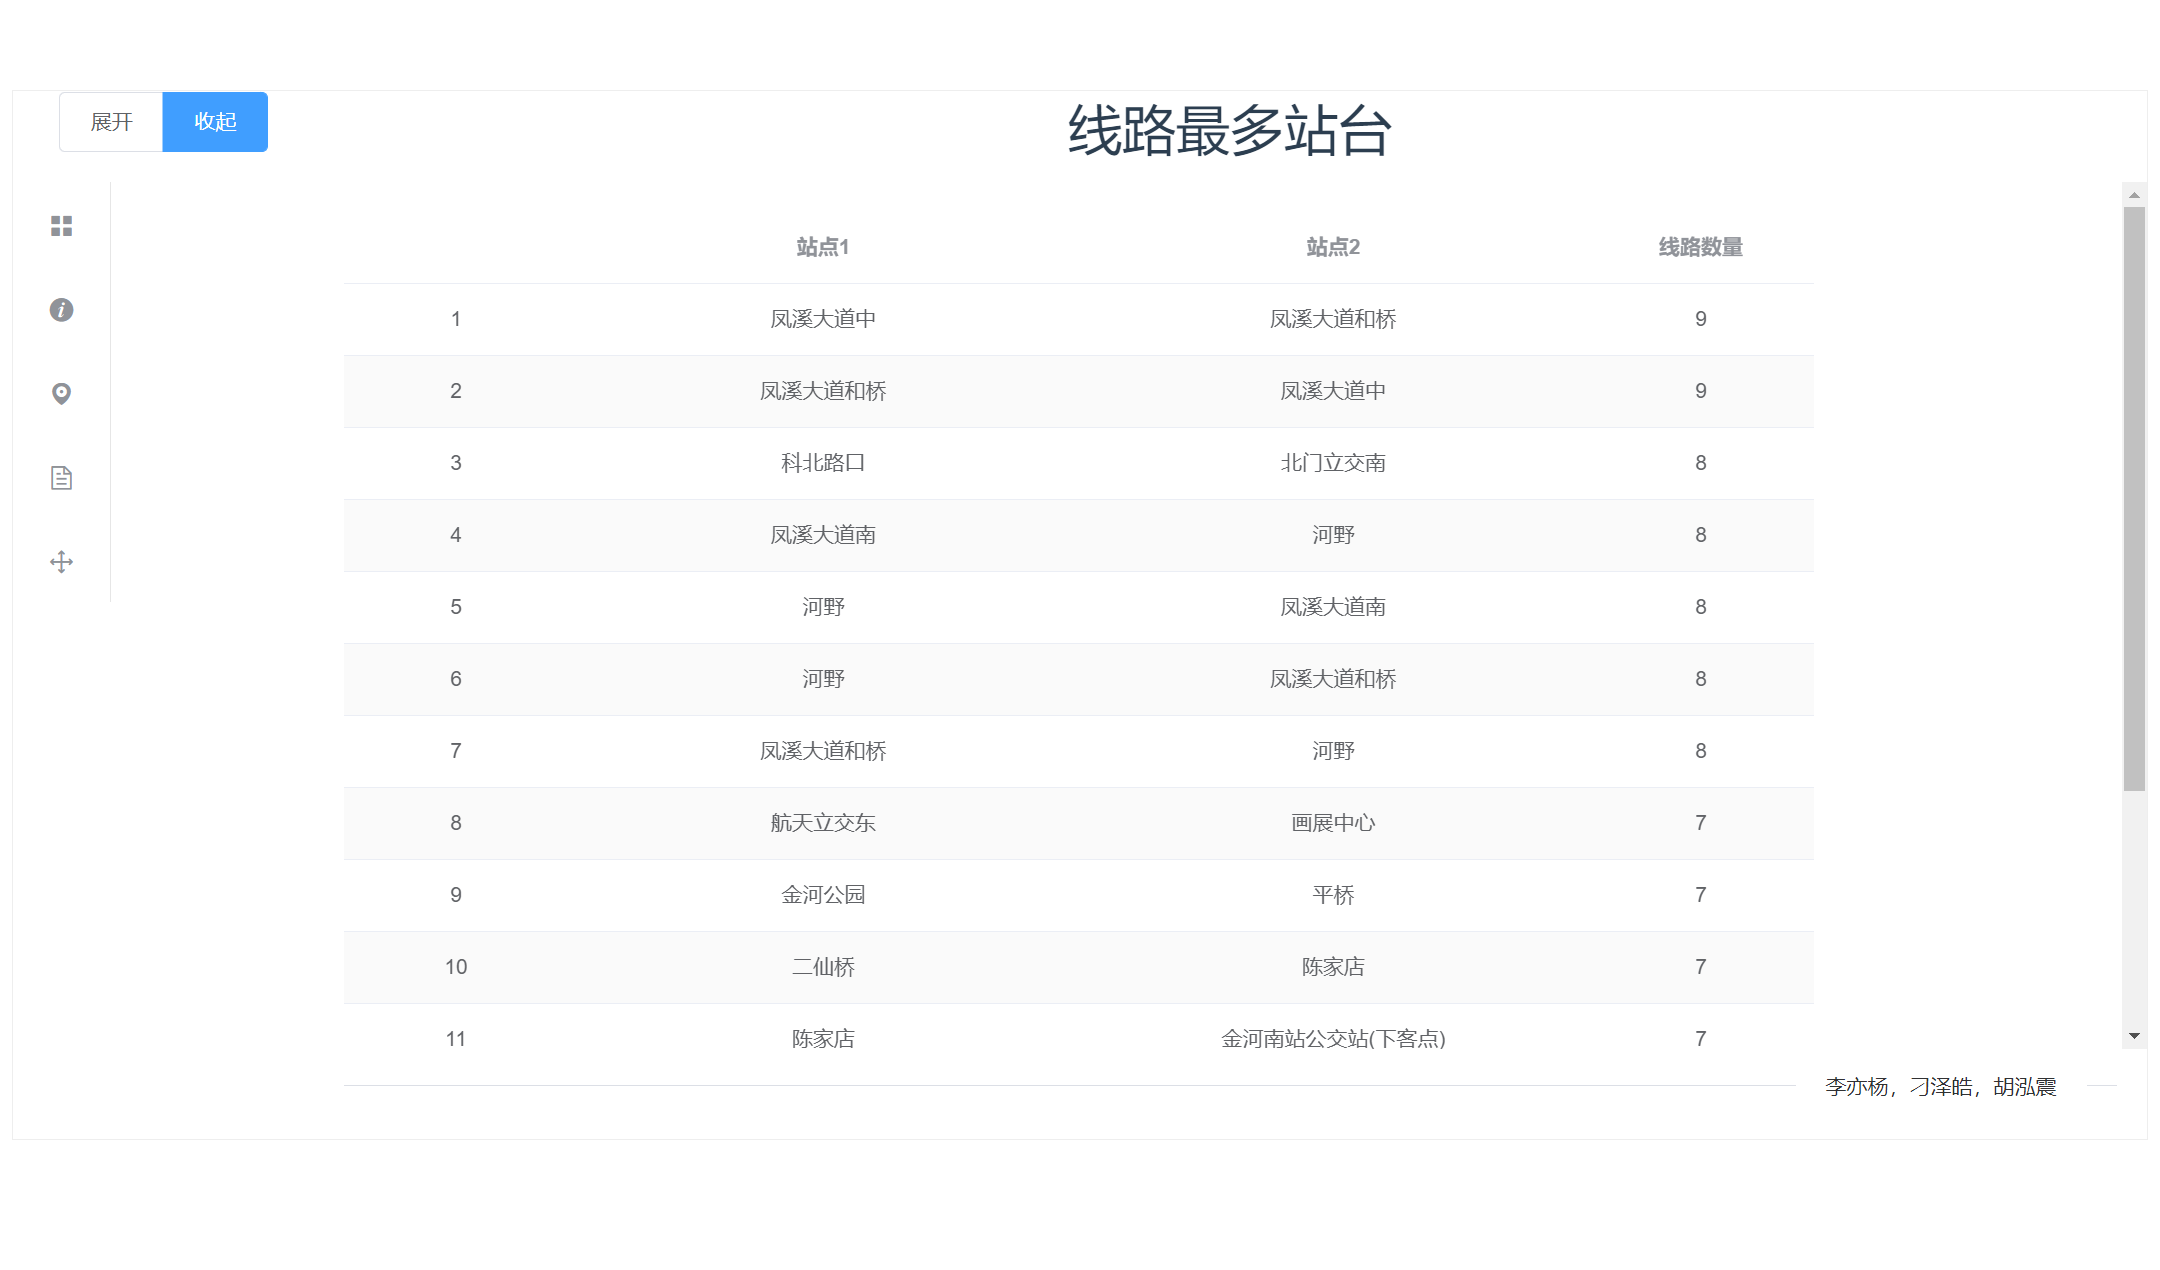
\includegraphics[scale=0.3]{./assets/demand15_1.png} \\ 
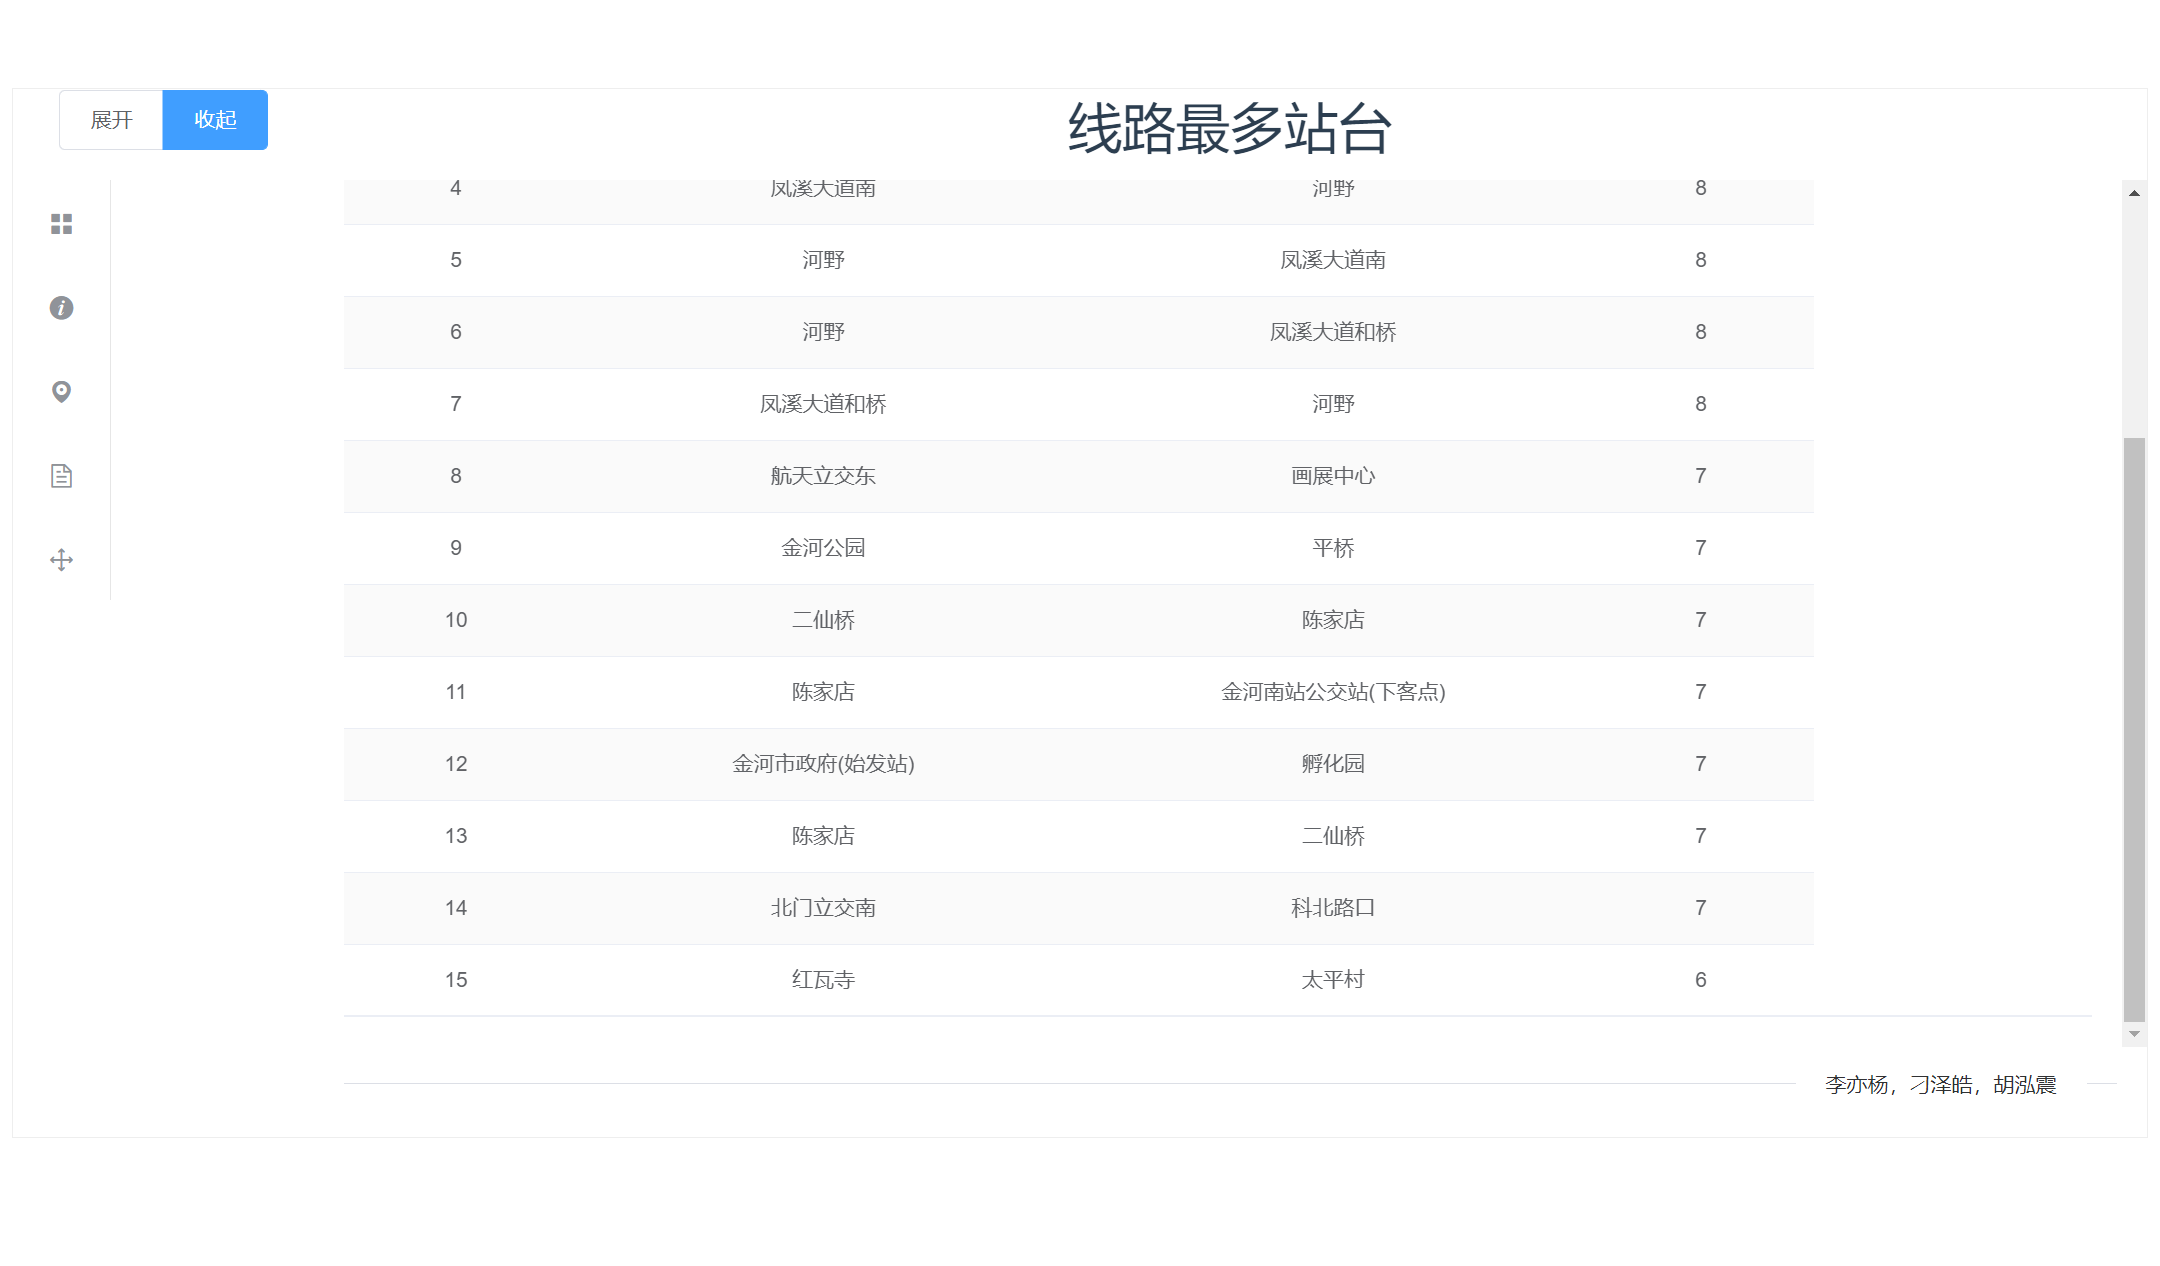
\includegraphics[scale=0.3]{./assets/demand15_2.png} 
\end{center}

\subsection{需求16}
\textbf{根据站点数量对线路(含方向)排序显示前15,返回线路名和对应站点数量。} \\
\textbf{Cypher} \\
\begin{lstlisting}[numbers = left, 
showstringspaces=false,
showspaces = false,
breaklines = true, 
language=Java]
@Query("""
	match (a:Line)
	with a, length(a.route) as cnt
	order by cnt desc
	return a.name limit 15
	""")
ArrayList<String> most_station_name();

@Query("""
	match (a:Line)
	with a, length(a.route) as cnt
	order by cnt desc
	return a.direction limit 15
	""")
ArrayList<String> most_station_direction();

@Query("""
	match (a:Line)
	with a, length(a.route) as cnt
	order by cnt desc
	return cnt limit 15
	""")
ArrayList<Integer> most_station_count();
\end{lstlisting} 
对所有Line节点,统计route内的元素个数,然后按个数降序返回前15个。\\
由于springboot不支持返回自定义类的集合,因此拆成三个函数。

\textbf{业务层} \\
\begin{lstlisting}[numbers = left, 
showstringspaces=false,
showspaces = false,
breaklines = true, 
language=Java]
	public JSONArray most_stations(){
        JSONArray arr = new JSONArray();

        ArrayList<String> res_name = stationrepository.most_station_name();
        ArrayList<String> res_direction = stationrepository.most_station_direction();
        ArrayList<Integer> res_cnt = stationrepository.most_station_count();
        ArrayList<Demand16> result = new ArrayList<>();

        if(!res_cnt.isEmpty()){
            for(int i = 0; i < res_cnt.size(); i ++){
                Demand16 dem = new Demand16();
                dem.name = res_name.get(i);
                dem.direction = res_direction.get(i);
                dem.count = res_cnt.get(i);
                result.add(dem);
            }
        }

        Demand16 res = new Demand16();
        if(!result.isEmpty()){
            for(int i = 0; i < result.size(); i ++){
                JSONObject obj = new JSONObject();
                res = result.get(i);
                if(Objects.equals(res.direction, "up"))
                    res.direction = "上行";
                else if(Objects.equals(res.direction, "down"))
                    res.direction = "下行";
                else if(Objects.equals(res.direction, "circle"))
                    res.direction = "环线";
                obj.put("route", res.name + "路" + res.direction);
                obj.put("num", res.count);
                arr.add(obj);
            }
        }
        return arr;
    }
\end{lstlisting} 
分别调用most$\_$station$\_$name,most$\_$station$\_$direction和most$\_$station$\_$count函数,返回两个字符串列表res$\_$name(线路名字),res$\_$direction(线路方向),和一个整数列表res$\_$cnt(线路中站点数量),列表的长度为15,是站点数前15位。将其整合为一个Demand16列表result。将其转化为JSONArray输出。


\textbf{前端界面测试结果} \\
\begin{center}
\centering
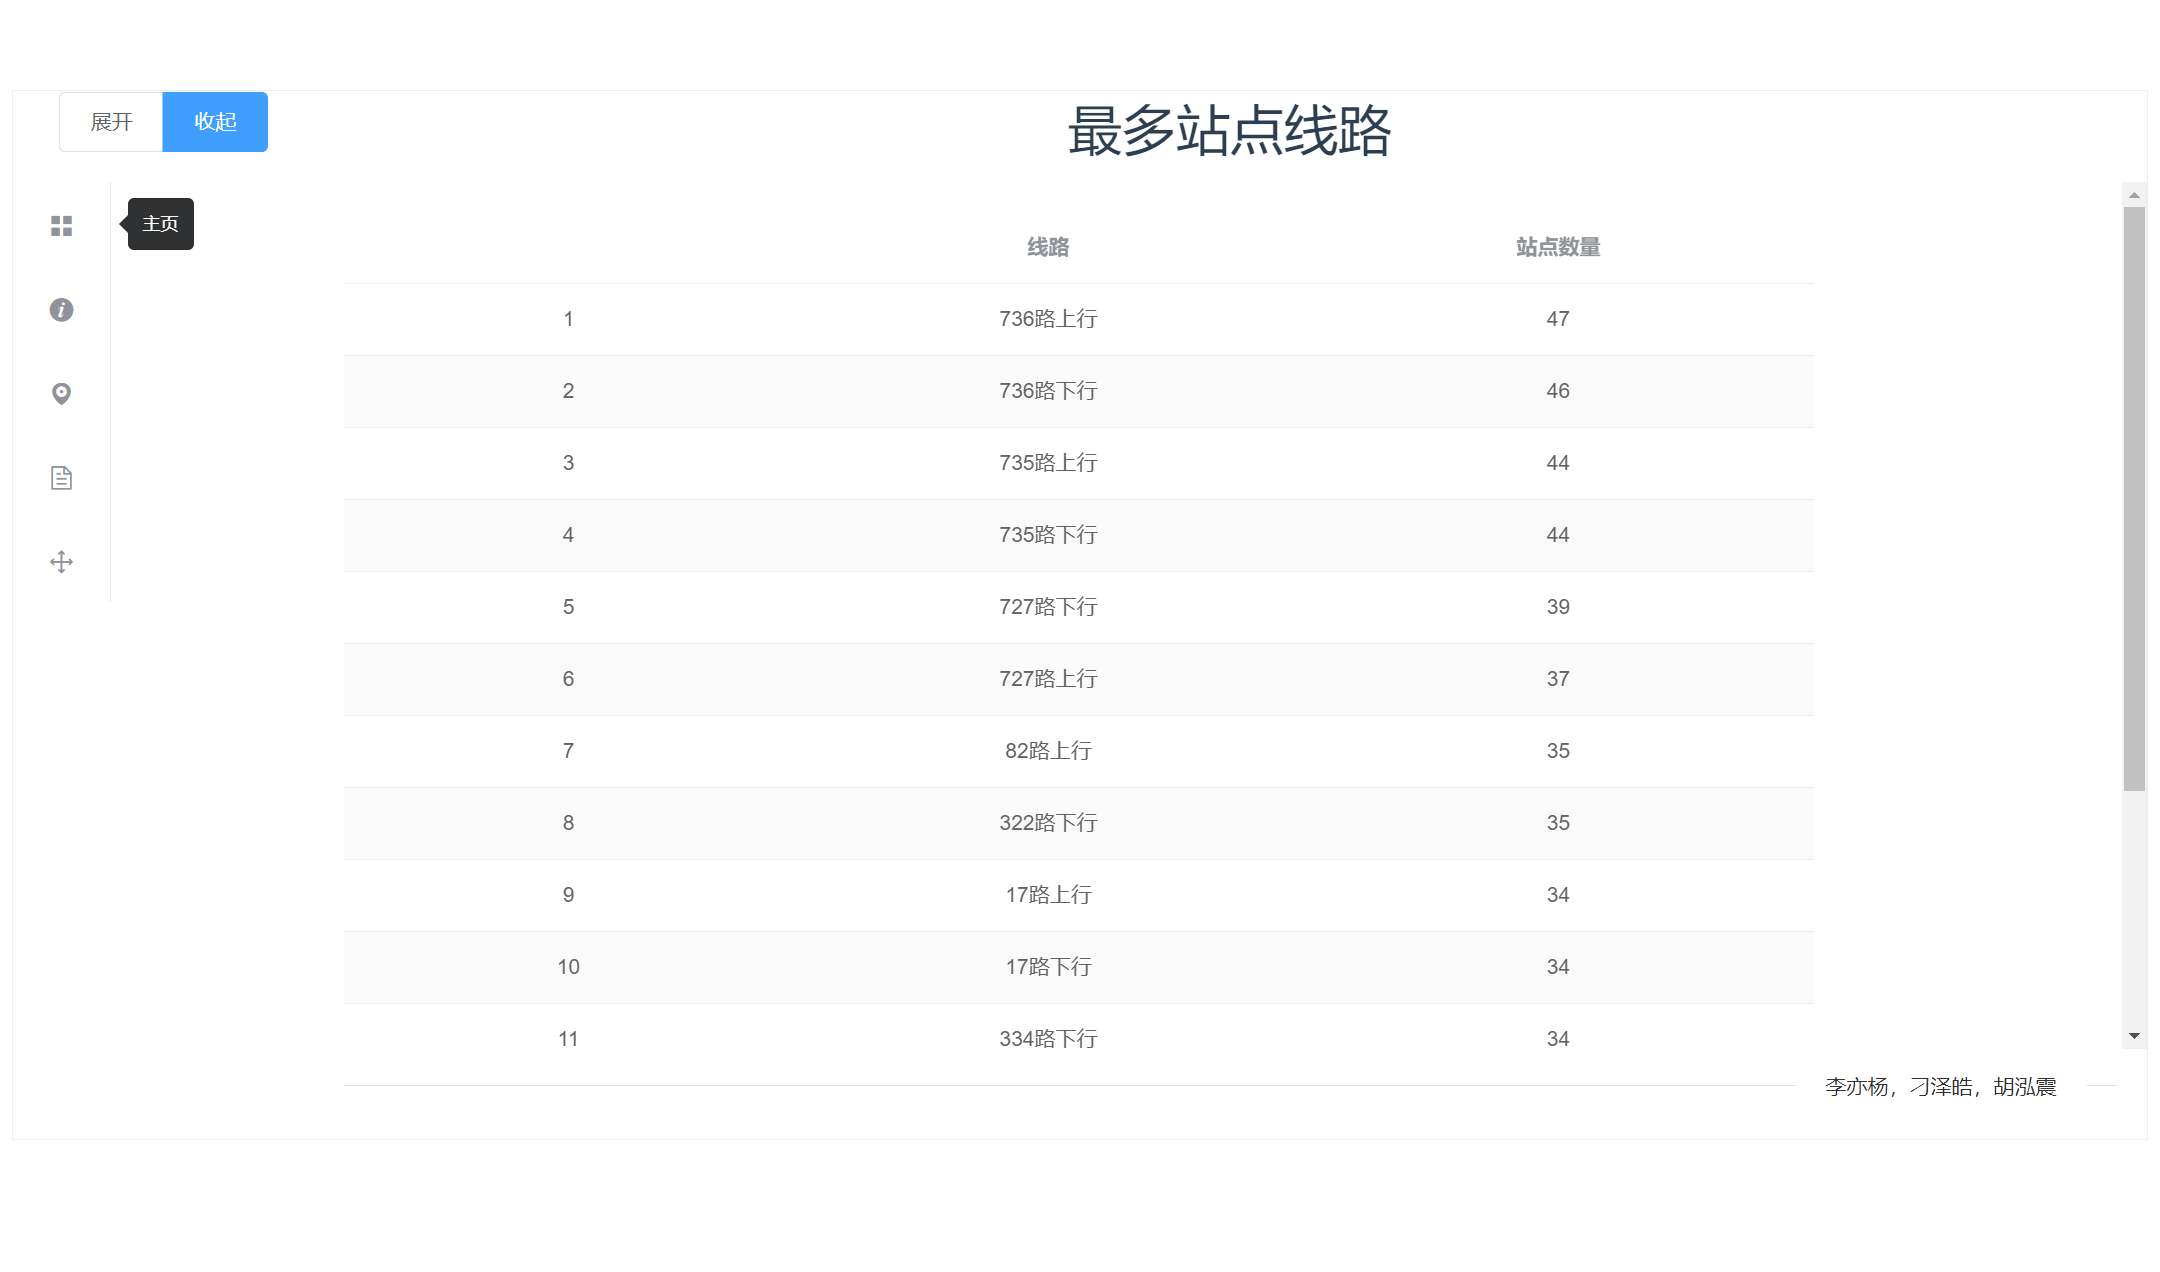
\includegraphics[scale=0.3]{./assets/demand16_1.png} \\ 
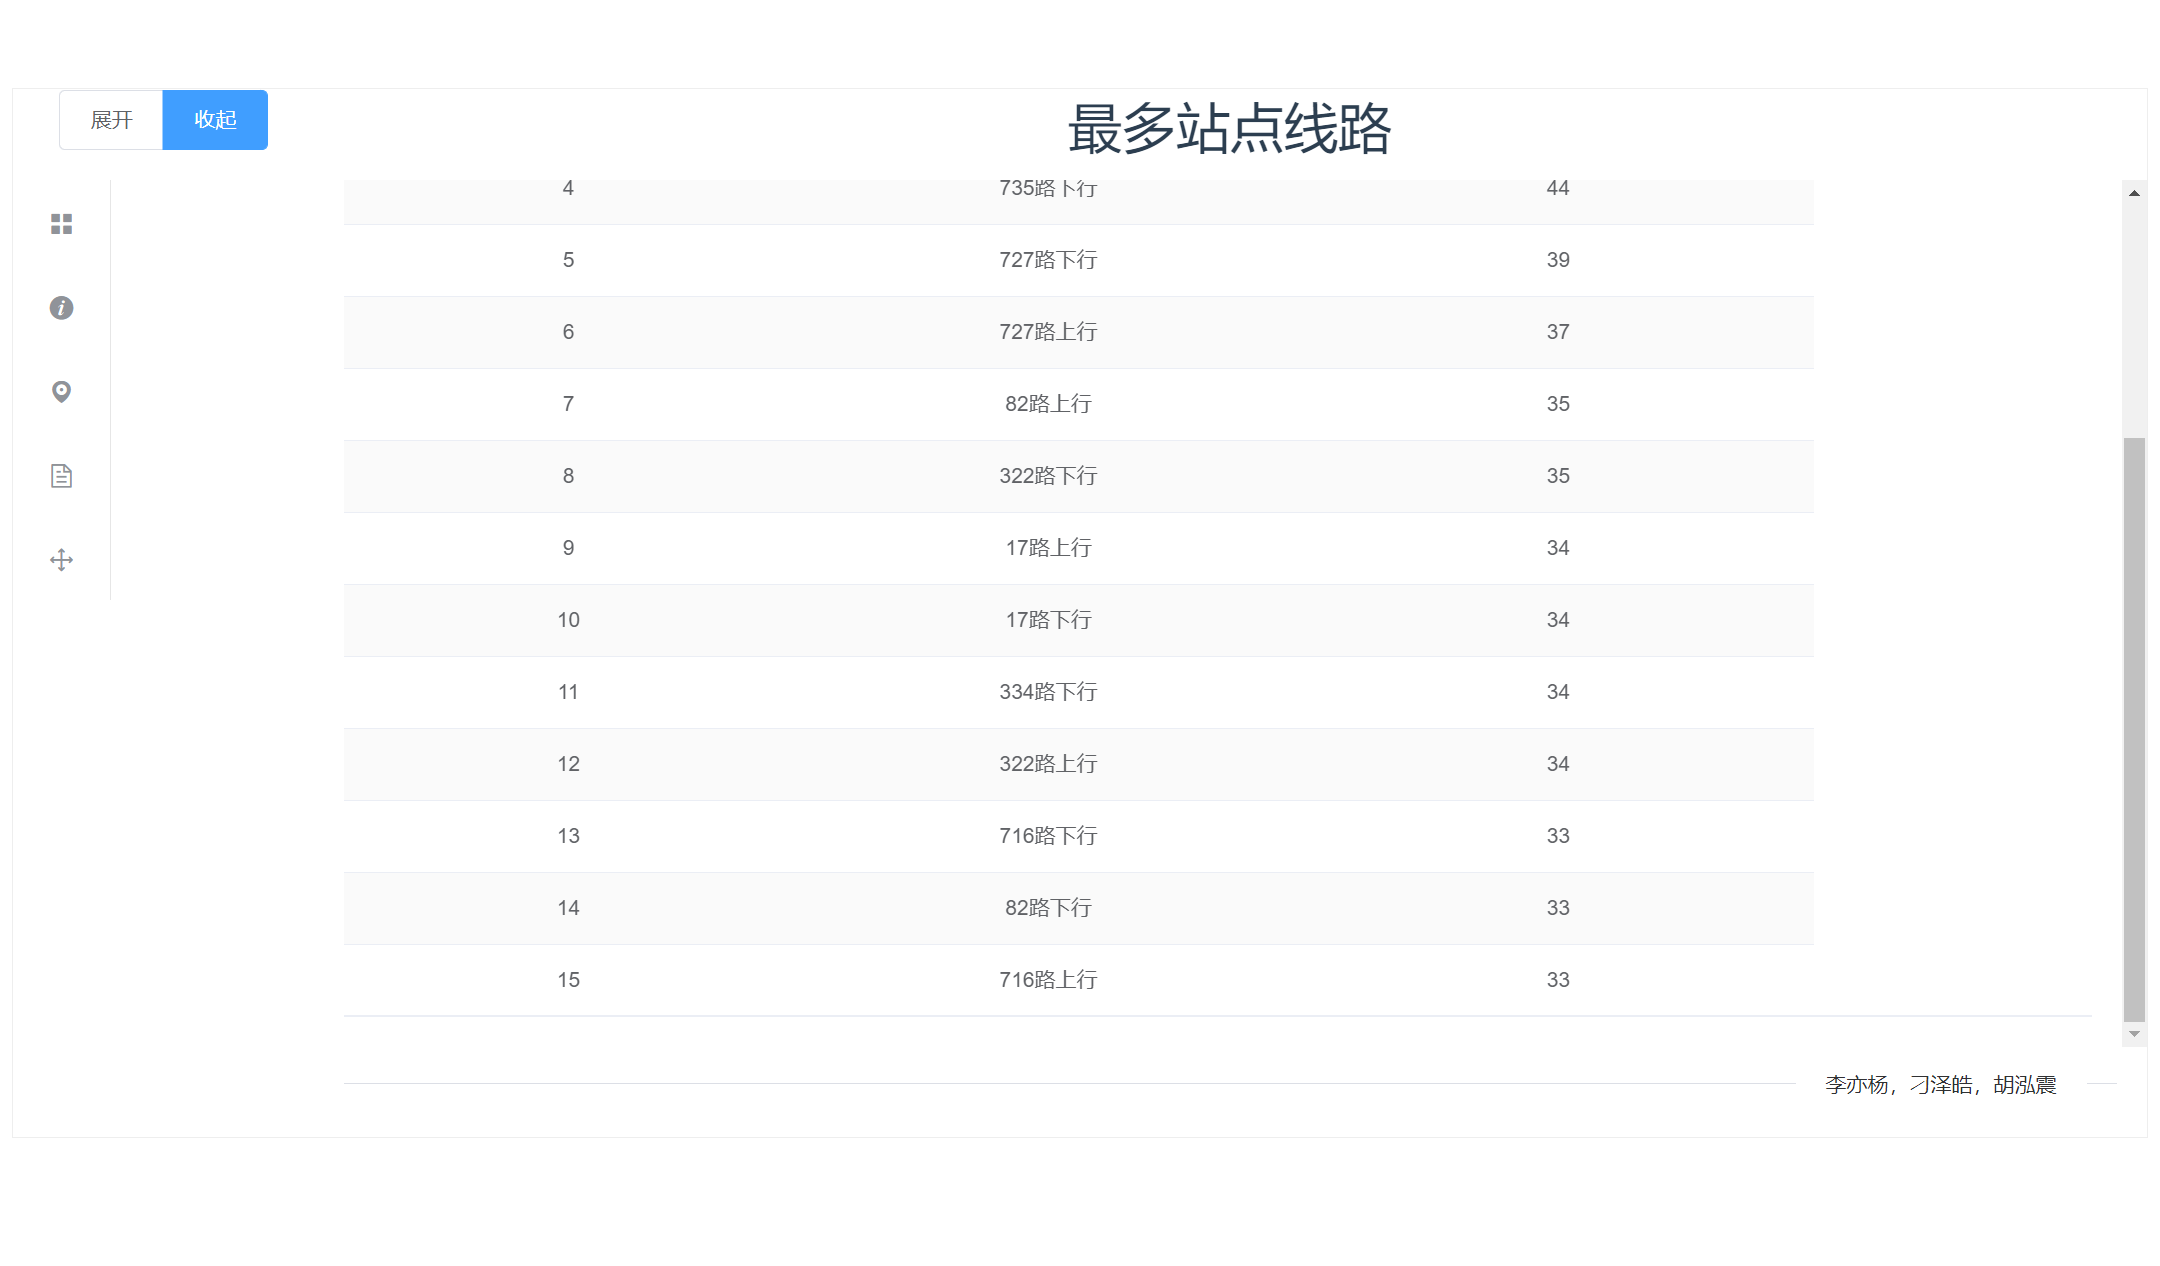
\includegraphics[scale=0.3]{./assets/demand16_2.png} 
\end{center}

\subsection{需求17}
\textbf{由班次数据计算出每班单程运行时间,对时间降序排列输出前15条。} \\
\textbf{Cypher} \\
\begin{lstlisting}[numbers = left, 
showstringspaces=false,
showspaces = false,
breaklines = true, 
language=Java]
@Query("""
	match
		(r:Run{line_id:{line_name}, direction: {line_direct}})
	return r.time[0] limit 1
	""")
String get_start_time_in_one_run(String line_name, String line_direct);

@Query("""
	match
		(r:Run{line_id:{line_name}, direction: {line_direct}})
	return r.time[-1] limit 1
	""")
String get_end_time_in_one_run(String line_name, String line_direct);
\end{lstlisting} 
第一个函数返回所有Line节点的名字,供service层调用剩下两个函数。 \\
第二个函数匹配指定名字和方向的Line节点,然后返回线路开始运行的时间。\\
第三个函数匹配指定名字和方向的Line节点,然后返回线路结束运行的时间。

\textbf{业务层} \\
\begin{lstlisting}[numbers = left, 
showstringspaces=false,
showspaces = false,
breaklines = true, 
language=Java]
    public JSONArray longest_time(){
        JSONArray arr = new JSONArray();
        ArrayList<Line> linenames;
        linenames = linerepository.get_all_line_names();

        ArrayList<Demand17> result = new ArrayList<>();

        if(!linenames.isEmpty()){
            for(int i = 0 ; i < linenames.size() ; i++)
            {
                String nam = linenames.get(i).getName();
                String direct = linenames.get(i).getDirection();
                String start_time = linerepository.get_start_time_in_one_run(nam, direct);
                String end_time = linerepository.get_end_time_in_one_run(nam, direct);
                SimpleDateFormat ft = new SimpleDateFormat ("HH:mm");
                Date t1;
                long l1;
                Date t2;
                long l2;
                int runtime;

                String dir = new String();
                if(Objects.equals(direct, "up"))
                    dir = "路上行";
                else if(Objects.equals(direct, "down"))
                    dir = "路下行";
                else if(Objects.equals(direct, "circle"))
                    dir = "路环线";

                nam += dir;

                Demand17 dem = new Demand17();
                dem.name = nam;

                try {
                    t1 = ft.parse(start_time);
                    l1 = t1.getTime();
                    t2 = ft.parse(end_time);
                    l2 = t2.getTime();
                    runtime = (int)((l2 - l1)/60000);
                    dem.time = runtime;
                } catch (ParseException e) {
                    System.out.println("Unparseable using " + ft);
                }

                result.add(dem);
            }
        }

        Collections.sort(result,new SortDemand17ByTime());

        ArrayList<Demand17> res = new ArrayList<>();

        for(int i = 0; i < 15; i ++){
            res.add(result.get(i));
        }

        if(!res.isEmpty()){
            for(int i = 0; i < res.size(); i ++){
                Demand17 tmp_dem = res.get(i);

                JSONObject obj = new JSONObject();
                obj.put("route", tmp_dem.name);
                obj.put("time", tmp_dem.time);
                arr.add(obj);
            }
        }
        return arr;
    }
}
\end{lstlisting} 
\begin{lstlisting}[numbers = left, 
showstringspaces=false,
showspaces = false,
breaklines = true, 
language=Java]
class SortDemand17ByTime implements Comparator {
    public int compare(Object o1,Object o2){
        if(((Demand17)o1).time < ((Demand17)o2).time)
            return 1;
        if(((Demand17)o1).time > ((Demand17)o2).time)
            return -1;
        return 0;
    }
}
\end{lstlisting} 
首先调用get$\_$all$\_$line$\_$names函数返回所有线路名称的列表linenames。然后创建一个Demand17(包含线路名称和运行时间两个属性)的列表result保存最终结果,对linenames中每一项调用get$\_$start$\_$time$\_$in$\_$one$\_$run和get$\_$end$\_$time$\_$in$\_$one$\_$run函数,返回其某一班次的起始和终止时间(字符串保存),将其通过Date类型转换为int,存入result列表中,对其进行排序。转化JSONArray对象输出。 \\
在本需求中,一开始我们将两个Query语句写在了一起,并输出到一个ArrayList<String>形的容器当中,然而一直报错。经过Debug我们发现,Query语句的映射也是有方向性的。倘若返回一组数据,会将一组数据的每一项都映射为ArrayList中的一项,而对每一项数据,考虑其为结构体或者说类的形式,Query语句中return后所跟的返回值的个数,应当与ArrayList中每一项数据内的数据种类相匹配。

\textbf{前端界面测试结果} \\
\begin{center}
\centering
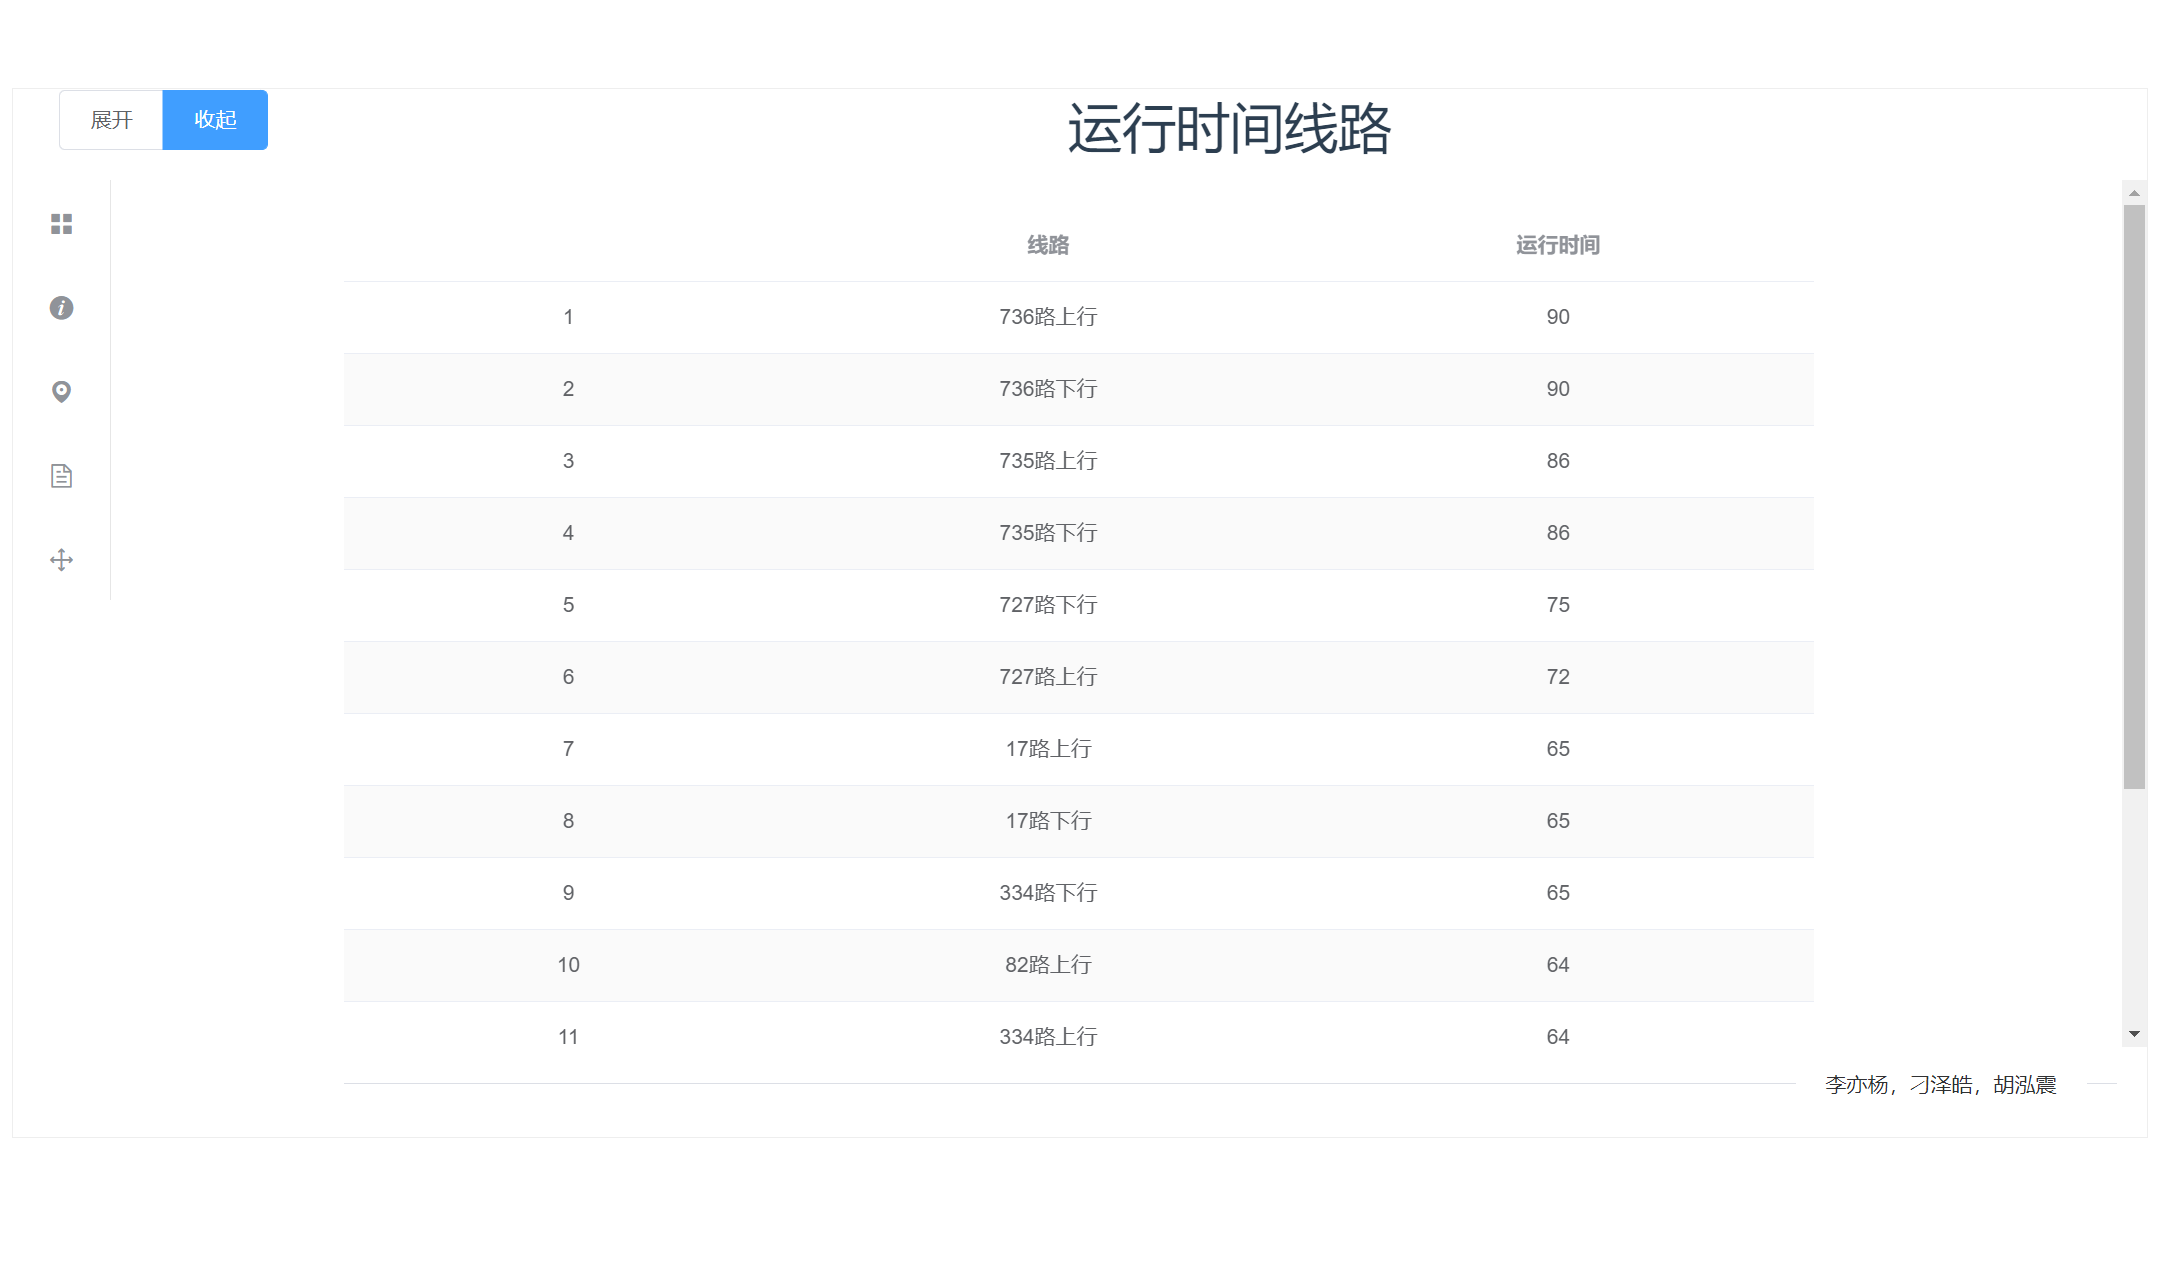
\includegraphics[scale=0.3]{./assets/demand17_1.png} \\ 
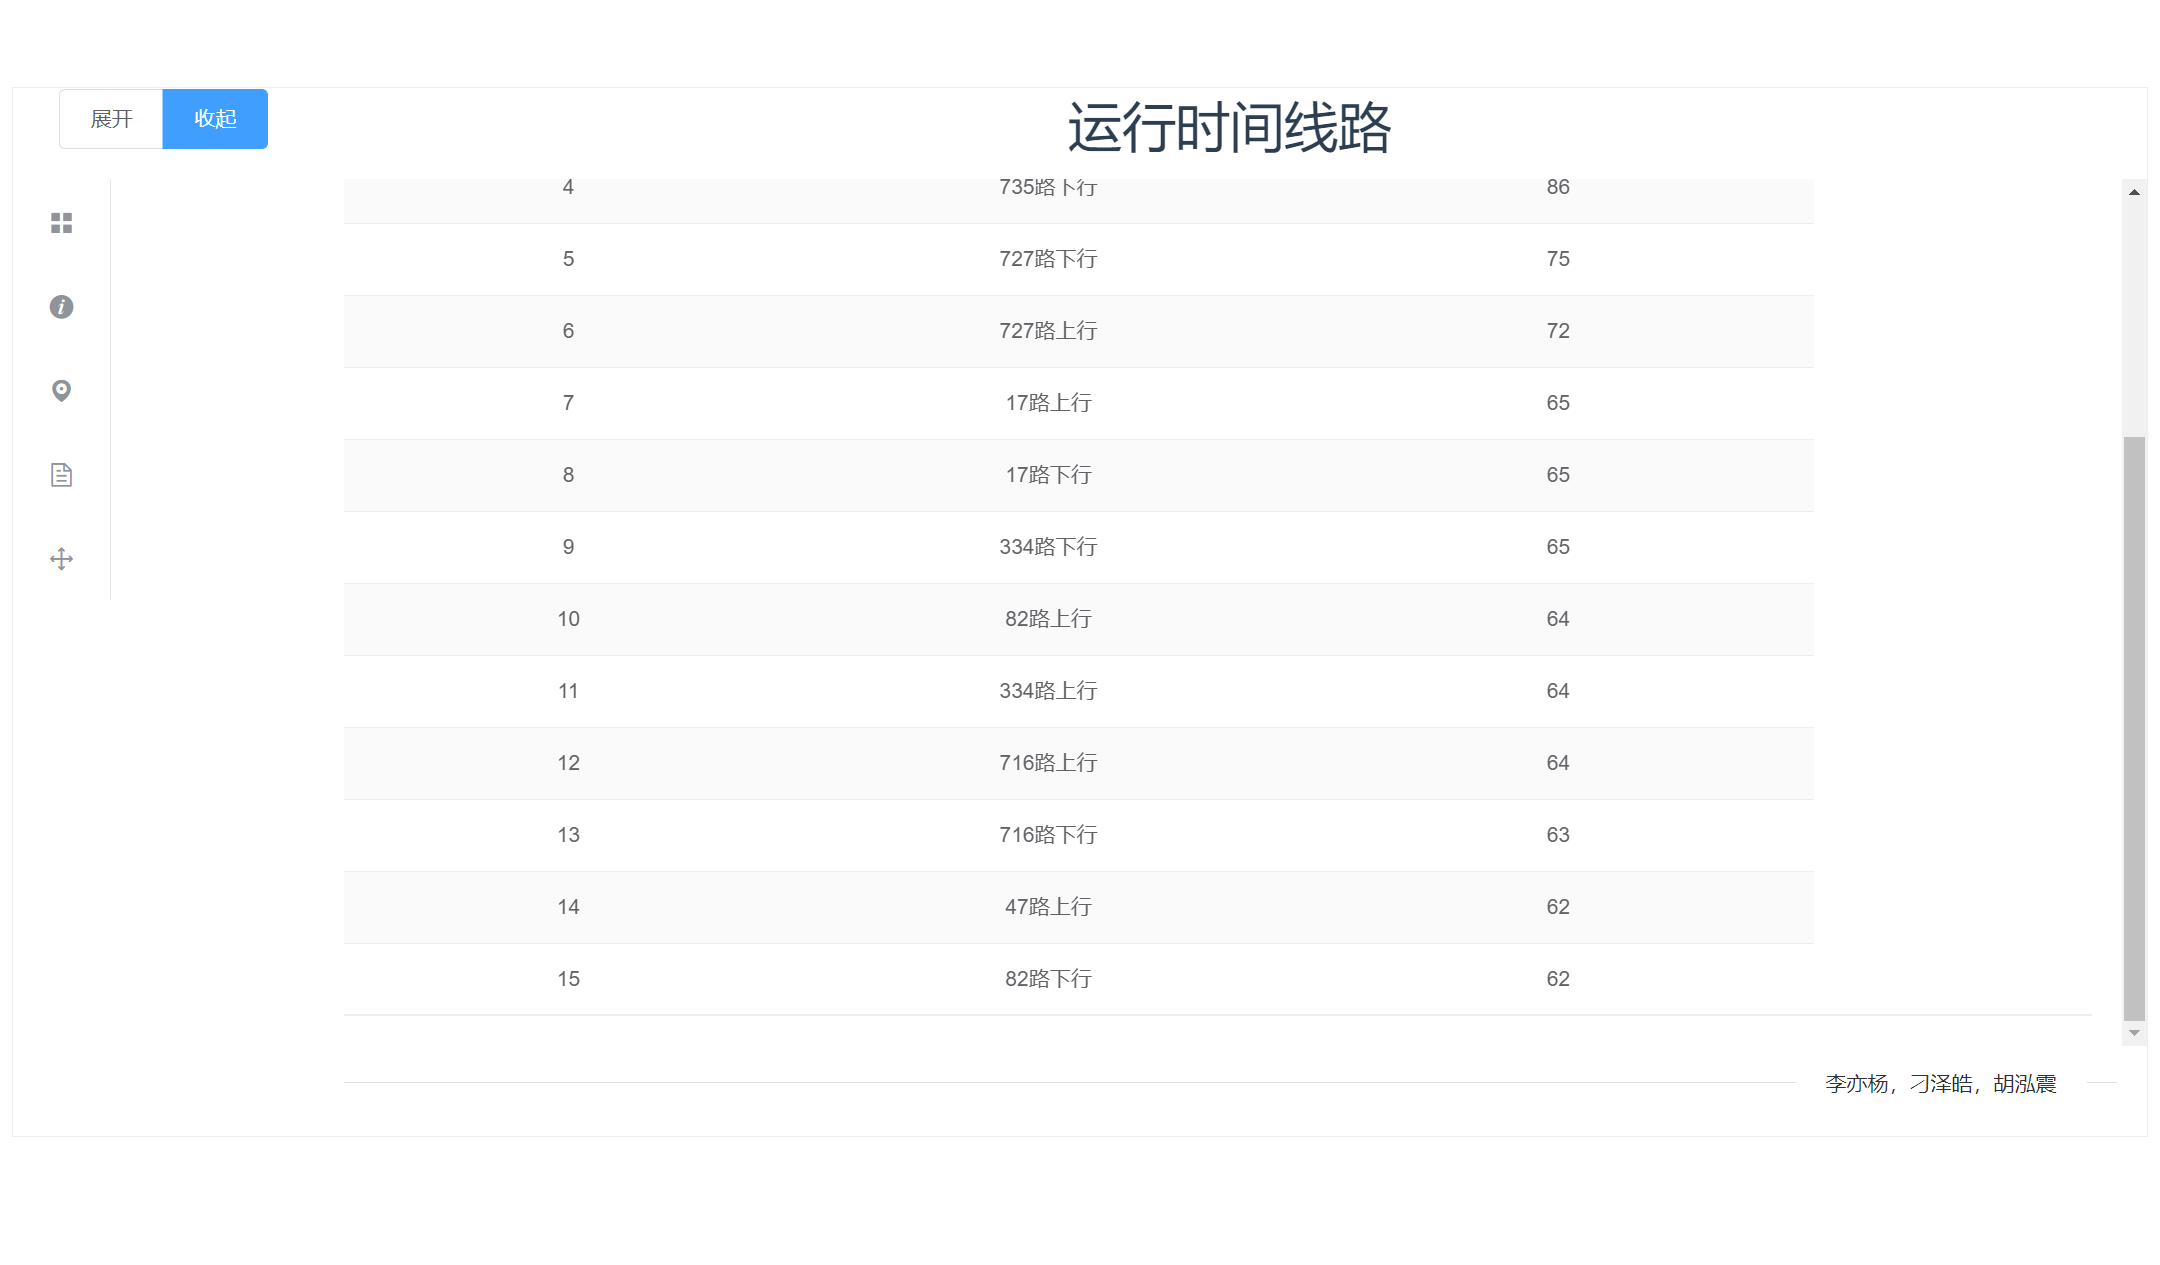
\includegraphics[scale=0.3]{./assets/demand17_2.png} 
\end{center}

\subsection{需求20}
\subsubsection{a}
\textbf{删除某条线路及其独占的站点} \\
\textbf{Cypher} \\
\begin{lstlisting}[numbers = left, 
showstringspaces=false,
showspaces = false,
breaklines = true, 
language=Java]
@Query("""
	match
		(n:Line {name:{line_id}})
	detach delete n
	match
		(r:Run{line_id:n.name})
	detach delete r
	match
		(a:Station) -[r]-> (b:Station) where n.name in r.lines and size(r.lines) = 1
	delete r
	match
		(a:Station) where not (a) -- ()
	delete a
	return n limit 1
	""")
Line delete_line(@Param("lien_id") String line_id);
\end{lstlisting} 
先查出要删除的线路,删除它和到它的所有BelongTo关系。 \\
再查出所有该线路的班次删除。 \\
接着查出所有Connection关系中lines里含有该线路的,从lines中删除,如果lines里没有其它线路,删除该Connection。\\
最后查出所有和其它站点都没有关系的站点,删除。

\textbf{业务层} \\
\begin{lstlisting}[numbers = left, 
showstringspaces=false,
showspaces = false,
breaklines = true, 
language=Java]
    public void delete_line(String lineId){
        linerepository.delete_line(lineId);
    }
\end{lstlisting} 
直接调用LineRepository中的delete$\_$line函数,传入线路id即可。

\textbf{前端界面测试结果} \\
\begin{center}
\centering
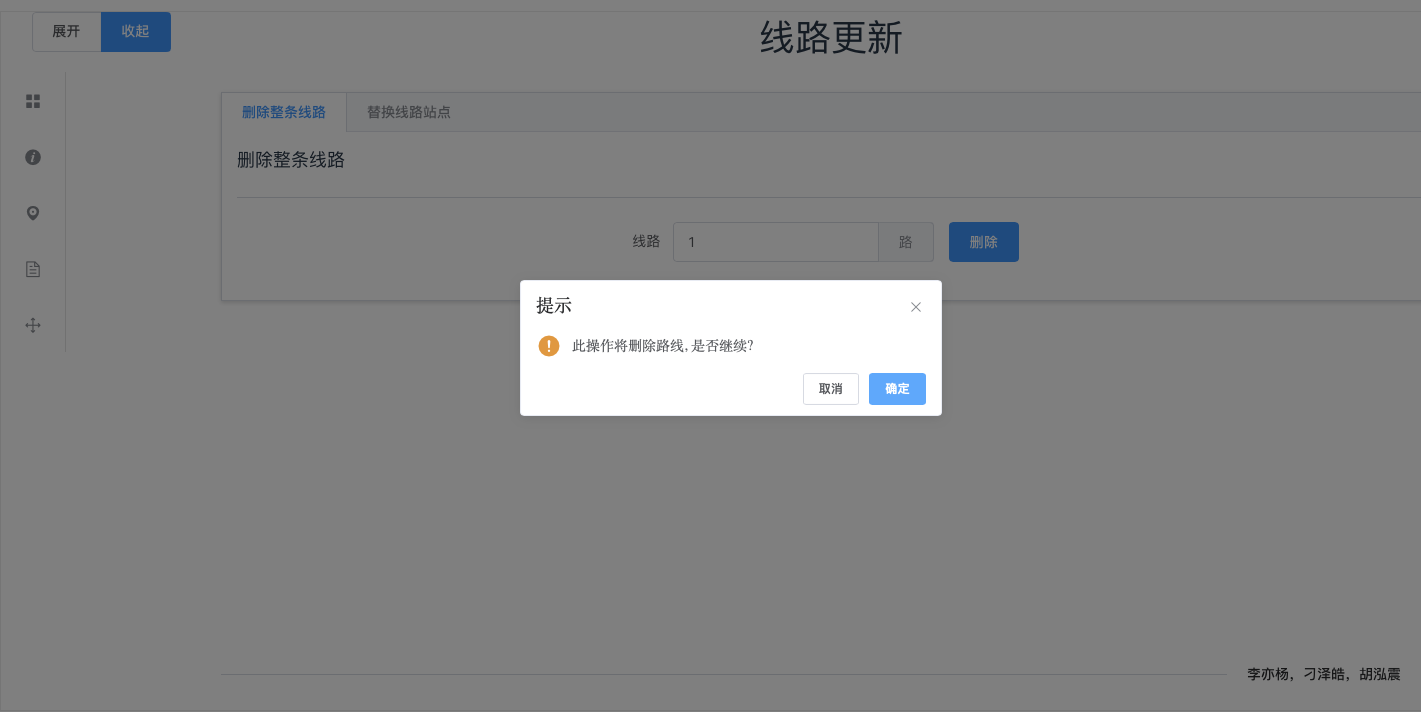
\includegraphics[scale=0.3]{./assets/demand20_1.png} \\ 
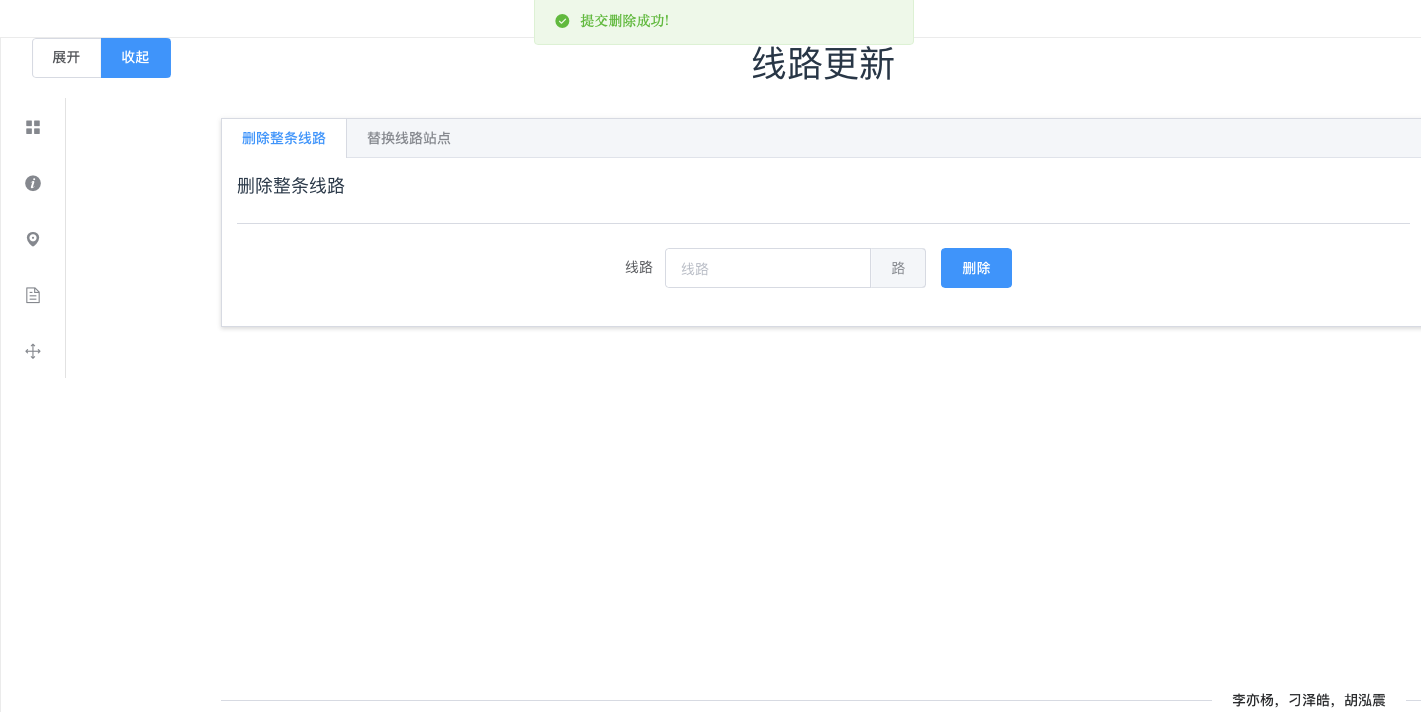
\includegraphics[scale=0.3]{./assets/demand20_2.png} 
\end{center}

\subsubsection{b}
\textbf{替换一条线路中某站点,返回更改后的线路中所有站点信息} \\
\textbf{Cypher} \\
\begin{lstlisting}[numbers = left, 
showstringspaces=false,
showspaces = false,
breaklines = true, 
language=Java]

\end{lstlisting} 
首先根据线路名和旧站点查出对应的线路,通过route属性反查出旧站点对应的索引,将索引给新站点的ID。\\
之后查出并删除前驱和后继站点到旧站点的Connection关系中lines属性里的对应线路,如果lines里因此没有元素,删除这个关系。\\
更新新站点到前驱和后继的关系。\\
如果旧站点因此不是任何关系的一端,则删除旧站点。

\textbf{业务层} \\
\begin{lstlisting}[numbers = left, 
showstringspaces=false,
showspaces = false,
breaklines = true, 
language=Java]
    public JSONArray change_line(String lineId,String direction,String stationId,String newStationId){
        linerepository.change_line(lineId, stationId, newStationId);
        JSONArray arr = new JSONArray();
        ArrayList<Station> station;
        station = stationrepository.find_route_station(lineId, direction);
        if(!station.isEmpty()){
            for(int i = 0; i<station.size();i++)
            {
                JSONObject obj = new JSONObject();
                Station s = station.get(i);
                obj.put("id",s.getId());
                obj.put("name",s.getName());
                obj.put("english",s.getEnglish());
                arr.add(obj);
            }
        }
        return arr;
    }
\end{lstlisting} 
调用LineRepository中的change$\_$line函数,传入lineId,stationId和newStationId参数。然后和需求二中完全相同,将更改后的线路站点信息返回。

\textbf{前端界面测试结果} \\
\begin{center}
\centering
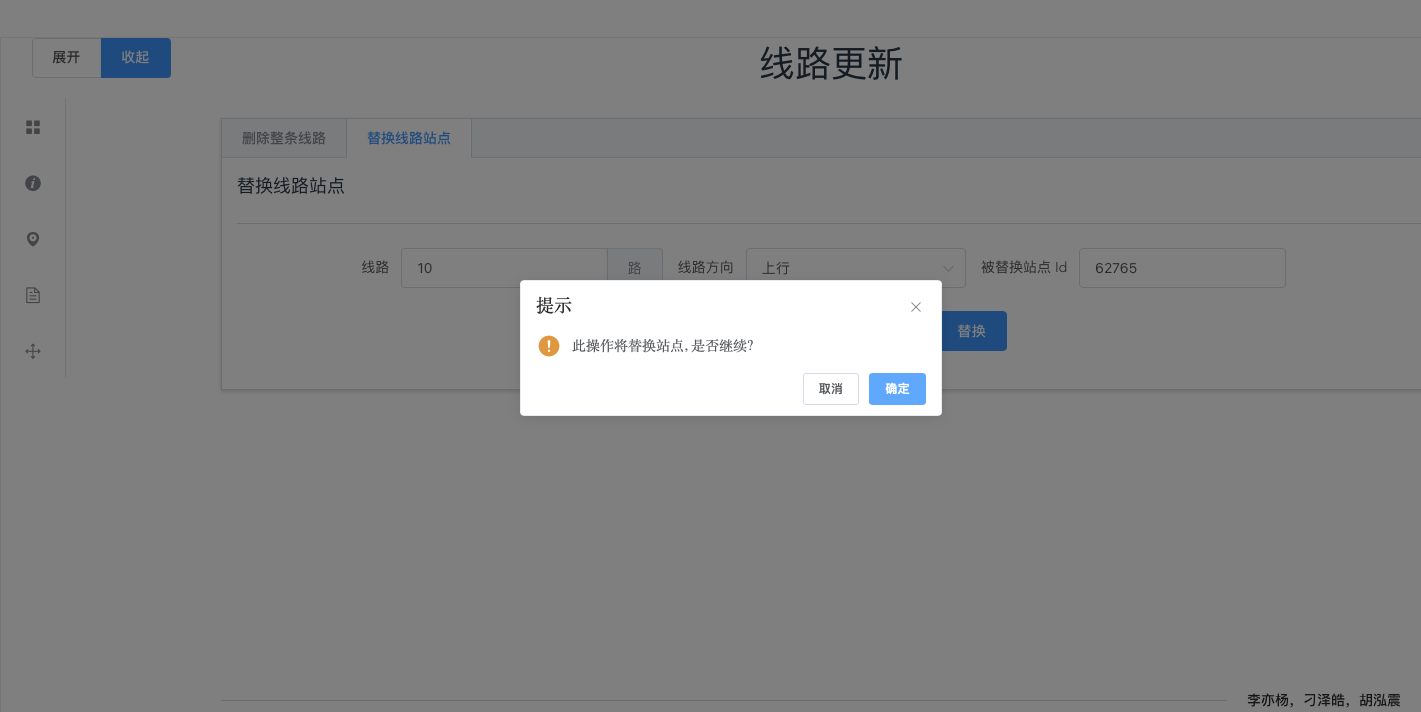
\includegraphics[scale=0.3]{./assets/demand20_3.png} \\ 
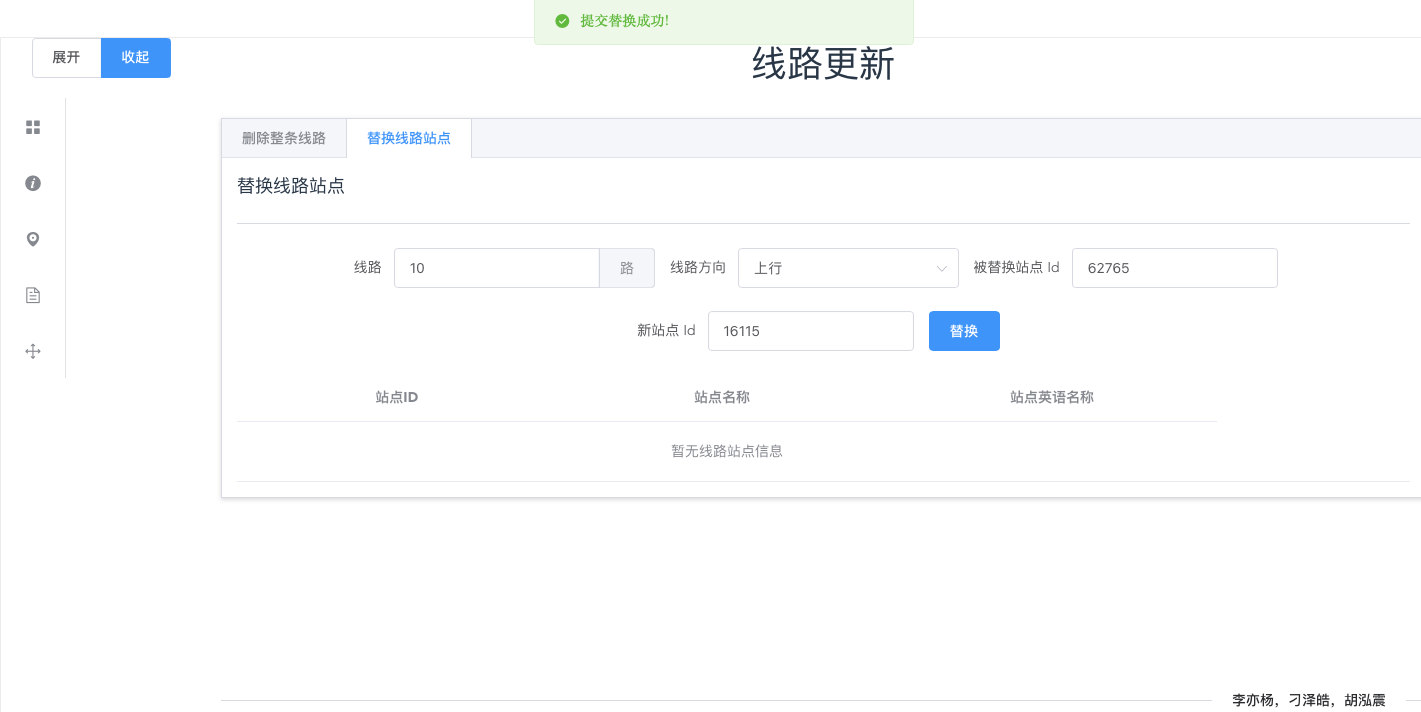
\includegraphics[scale=0.3]{./assets/demand20_4.png} 
\end{center}

\section{项目代码}
由于小组成员分工较为明确,基本不会有同一行或一个文件的代码上的编辑冲突,为了方便小组成员修改后项目的版本控制,我们组建了一个Github仓库。考虑到项目报告并不需要提交整个项目的代码,因而在此附上我们项目的Github仓库链接,便于老师查阅。 \\
项目Github仓库如下:\\
\url{https://github.com/pikapikapikaori/NoSQL}

\end{document}
%==================================================
%%%%%%%%%%%%%%%%%%%%%%%%%%%%%%%%%%%%%%%%%%%%%%%%%%%